% !TEX root =  manuscript_arxiv.tex

\counterwithin{equation}{section}
\counterwithin{figure}{section}
\renewcommand{\thefigure}{\Alph{section}.\arabic{figure}}
\counterwithin{table}{section}
\renewcommand{\thetable}{\Alph{section}.\arabic{table}}
\counterwithin{theorem}{section}
\renewcommand{\thetheorem}{\Alph{section}.\arabic{theorem}}
\counterwithin{lemma}{section}
\renewcommand{\thelemma}{\Alph{section}.\arabic{lemma}}


\begin{center}
    \LARGE \textbf{Supplementary Materials}
\end{center}

%\begin{lemma}
%	Suppose $\mathcal{I}$ and $\mathcal{I}'$ are two disjoint sets for $\{1,\ldots, K\}$. For two sets of coefficients $a_k, b_{k'}$, suppose $a_k\neq0$ for $k \in \mathcal{I}$, $a_k=0$ for $k \in \mathcal{I}'$,  $b_{k'}=0$ for $k' \in \mathcal{I}$ and $\sum_{k\in \mathcal{I}} a_k = 1$ and $\sum_{k'\in \mathcal{I}'}b_{k'} = 1$. Then there exist coefficients $\gamma_{kk'}$ such that $\sum_{k\in\mathcal{I}, k'\in\mathcal{I}'}\gamma_{kk'}=1$.
%	
%\end{lemma}


\section{[out-of-date] Robust Model Selection Consistency} % of Structurally Aware Robust Model Selection
\label{sec:theory}

\PROBLEM{TODO: integrate material from this section into the appendix}

We now show that, under reasonable assumptions, our model selection procedure is robustly consistent.
Then, in light of our results, we discuss some specific choices of discrepancy measure.
Here we emphasize the assumptions required in the mixture modeling case, since the probabilistic matrix factorization assumptions are similar but require more notation to state;
see \cref{sec:PMF-consistency-proof} for details.

\subsection{Assumptions}


%We now show that our model selection procedure consistently estimates $K_{o}$ under reasonable assumptions.

%Let $\mcX$ and $\paramspace$ be spaces for observations and parameters, respectively. Assume family of distributions $\mathcal{F} = \{f_{\param}: \param \in \paramspace\}$ where $f_{\param}$ are absolutely continuous with respect to some base measure $\lambda$ on $\paramspace$.
%Denote the true number of components as $\numcomps_o$ and $F_{ok}$ as the true underlying distribution for component $k = 1, \ldots, \numcomps_o$. 
%We show that  structurally aware model selection rule achieves the consistency of number of components.
%Our assumptions are mild. 
First, we consider the requirements for the discrepancy $\discr{\cdot}{\cdot}$ and, when applicable, the discrepancy estimator $\discrest{\cdot}{\cdot}$
-- noting that sometimes it will be possible to take $\discrest{\cdot}{\cdot} = \discr{\cdot}{\cdot}$.
%We require the smoothness and the existence of a consistent estimator for discrepancies $\discr{P}{Q}$.
For some discrepancies such as the Kullback--Leibler divergence, $\discr{P}{Q} < \infty$ only if $P$ is absolutely continuous with respect to $Q$.
However, since we require an empirical estimate of each component distribution, absolute continuity may not hold.
Therefore, we introduce a possibly weaker metric $d$ on probability measures that detects convergence of empirical measures.
%satisfies $d(P, Q_{N}) \to 0$ as $N \to \infty$
%whenever $Q_{N} \to P$ in distribution. %   such which converges to zero whenever $Q$ converges to $P$ in distribution and can be bounded by a function of $\discr{P}{Q}$. 
%We also require some other modest regularity conditions on $d$ and $\mcD$, presented in \cref{assump:metric-discr-conditions}.
\begin{assumption} 	\label{assump:metric-discr-conditions}
	%Let $y_{1}, y_{2}, \dots$ be independent samples from distribution $P$, and denote 
	For $y_{\numobs n} \in \mathcal{X}$ $(\numobs = 1,2,\dots; n = 1,\dots,\numobs)$,
	define the empirical distribution $\widehat{P}_{\numobs} = \numobs^{-1}\sum_{n=1}^{\numobs}\delta_{y_{N,n}}$
	and assume $\widehat{P}_{\numobs} \rightarrow P$ in distribution.
	The metric $d$, discrepancy $\mcD$, and estimator $\widehat{\mcD}$ satisfy the following conditions:
	%\begin{enumerate}[(a)]
	\begin{enumerate}[label=\textnormal{(\alph*)}]
		\item \emph{The metric detects empirical convergence:} $d(\widehat{P}_\numobs, P) \to 0$ as $\numobs \to \infty$.
		\item  \emph{The metric is jointly convex in its arguments:} for all $w \in (0, 1)$ and distributions $P$, $P'$, $Q$, $Q'$,
		      \[
			      d(wP + (1 - w)P', wQ + (1 - w)Q') \le w\,d(P, Q) + (1 - w)\,d(P', Q').
		      \]
		      %$d(\sum_{i=1}^{n}w_i P_i, \sum_{i=1}^{n}w_i Q_i) \leq \sum_{i=1}^{n} w_i d(P_i, Q_i)$ for $0\leq w_i \leq 1$ and $\sum_{i = 1}^n w_i = 1$;
		      %	\item  \emph{The metric is bounded:} there exists a constant $M < \infty$ such that
		      %	$d(P,Q) \le M$ for all distributions $P, Q$. 
		\item  \emph{The discrepancy estimator is consistent:} For any distributions $P, Q$,
		      if $\discr{P}{Q} < \infty$ and $\widehat P_{N} \to P$ in distribution,
		      then $\discrest{\widehat{P}_{\numobs}}{Q} \to \discr{P}{Q}$ as $\numobs \to \infty$.
		\item \emph{Smoothness of the discrepancy estimator:} The map $\param \mapsto \discrest{\widehat{P}_{\numobs}}{F_{\param}}$ is continuous.
		\item  \emph{The discrepancy bounds the metric:} There exists a continuous,
		      non-decreasing function $\kappa: \reals \to \reals$ such that
		      $d(P,Q) \leq \kappa(\discr{P}{Q})$ for all distributions $P, Q$.
		\item \emph{The metric between components is finite:} For all $\param, \param' \in \Theta$,
		      we have $d(F_{\param}, F_{\param'}) < \infty$.
	\end{enumerate}
\end{assumption}

A wide variety of metrics satisfy \cref{assump:metric-discr-conditions}(a), including the bounded Lipschitz metric,
the Kolmogorov metric, maximum mean discrepancies with sufficiently regular bounded kernels, and the Wasserstein metric with a bounded cost function \citep{Vaart:1996,Sriperumbudur:2010,SimonGabriel:2018,Villani:2009}.
%requires metric $d$ to characterize the convergence of empirical process. For example, all metrics fall into the Glivenko--Cantelli class are able to provide the uniform convergence of empirical average to the true distribution in probability. This generally holds for a range of metrics including bounded Lipschitz and Kolmogorov metrics by \citep{Vaart:1996}.
%\cref{assump:metric-discr-conditions}(b) and \cref{assump:metric-discr-conditions}(c) admit the joint convexity and the boundedness of the metric, respectively. 
%The joint convexity property
\Cref{assump:metric-discr-conditions}(b) also holds for a range of metrics.
%For example, define integral probability metrics as 
%$\gamma_{\mathcal{H}}(P,Q) = \sup\{\vert \int_S f dP - \int_S f dQ \vert: f \in \mathcal{H} \}$, where $P$ and $Q$ are probability measures defined on space $S$ and $\mathcal{H}$ is a class of real-valued bounded measurable functions on $S$. 
For example, it is easy to show that all integral probability metrics -- which includes the bounded Lipschitz
metric, maximum mean discrepancy, and 1-Wasserstein distance -- are jointly convex (see \cref{lem:ipm-joint-convex} in the Appendix).
\cref{assump:metric-discr-conditions}(c) is a natural requirement that the limiting divergence can be estimated consistently.
Such estimators are well-studied for many common discrepancies.
%We discuss consistent estimation of the Kullback--Leibler divergence in \cref{sec:kl-estimation}.
\cref{assump:metric-discr-conditions}(d) will typically hold as long as the map $\phi \mapsto F_{\phi}$ is
well-behaved.
For example, for the Kullback--Leibler divergence estimators described in \cref{sec:kl-estimation}
and standard maximum mean discrepancy estimators \citep{Gretton:2012,Krause:2023},
when $F_{\phi}$ admits a density $f_{\phi}$, it suffices for the map $\phi \mapsto f_{\phi}(x)$
to be continuous for $P_{o}$-almost every $x$.
\cref{assump:metric-discr-conditions}(e) is not overly restrictive and we discuss some relevant examples in \cref{sec:divergence-choice} below.
%. See \citet{Gibbs:2002} for a extensive overview
%of the relationships between common metrics and divergences.
\cref{assump:metric-discr-conditions}(f) trivially holds for bounded metrics such as the bounded Lipschitz metric and integral probability measures with uniformly bounded test functions.

Our second assumption requires the parameter estimation procedure to be sufficiently well-behaved,
in the sense that, for each fixed number of components $\numcomps$, it should consistently estimate an asymptotic parameter $\allparam_{\star}^{(K)}$.
We do not make any explicit assumptions that such parameters are, in any sense, ``optimal.''
% quantifies the regularity of the inference algorithm and provides guarantees on contracting the convergence of empirical distribution to its limiting distribution.

\begin{assumption}\label{assump:inference-regularity}
	For each $\numcomps \in \{1,\dots, \numcomps_{o}\}$, there exists $\theta_{\star}^{(K)} \in \paramSpace{K}$ such that
	$\widehat\theta^{(K)} \to \theta_{\star}^{(K)}$ in probability as $N \rightarrow \infty$,
	after possibly reordering of components.
\end{assumption}
To simplify notation, we will write $F^{(K)}_{\star k} = F_{\param^{(K)}_{\star k}}$ and $G^{(K)}_{\star k} = G_{\allparam^{(K)}_{\star k}}$, and similarly for their densities.
\Cref{assump:inference-regularity} holds for most reasonable algorithms, including expectation--maximization, point estimates based on the posterior distribution,
and variational inference \citep{Balakrishnan:2017,Walker:2001,Wang:2019}.
Note that we assume that consistency holds for parameters in the equivalence class induced by component reordering, although we keep
this equivalence implicit.
\Cref{assump:inference-regularity} implies that the empirical data distribution of the $k$th component,
$\widehat{F}^{(K)}_k$, % = |X_{k}(z^{(K)})|^{-1}\sum_{x \in X_{k}(z^{(K)})} \delta_{x}$,
converges to a limiting distribution
% $\widetilde{P}^{(K)}_k$ that depends on $P_{o}$ and the limiting 
%parameters $\allparam_{\star}^{(K)}$:
%For fixed $\numcomps$ and each $k \in \{1,\dots,\numcomps\}$, denote the empirical weights and component distributions 
%by, respectively, $\eta^{(K)}_{\star k} = |X_{k}(z^{(K)}_{1:N})|/\numobs$
%and . 
%Define $\widetilde{F}^{(K)}_k$ as the limiting distribution of $\widehat{F}^{(K)}_k$ as
\begin{align}
	\widetilde{F}^{(K)}_{k}(\dee x) & = \frac{p_{\star}^{(K)}(k\mid x)P_o(\dee x) }{\int p_{\star}^{(K)}(k\mid y)P_o(\dee y)}, \label{eq:phat-def}
\end{align}
where $p_{\star}^{(K)}(k \mid x) = \eta^{(K)}_{\star k}f_{\star k}^{(K)}(x)/p^{(K)}_{\star}(x)$ is the
conditional component probability under the limiting model distribution.
%The limiting distribution $\widetilde{P}^{(K)}_k$ depends on the optimal parameter from the inference algorithm. 

%Denote the model optimal weights and distributions as $\eta_k^\star$ and $F^{\star}_{k}  (k=1, \ldots, \numcomps)$. 

Our third assumption concerns the regularity of the data distribution and model.
\begin{assumption} \label{assump:model-conditions}
	The data-generating distribution $P_o$ and component model family $\mcF$ satisfy the following conditions:
	%\begin{enumerate}[(a)]
	\begin{enumerate}[label=\textnormal{(\alph*)}]
		\item \emph{Meaningful decomposition of the data-generating distribution:} for positive integer $\numcomps_{o}$, $\eta_{o} \in \Int{\Delta_{\numcomps_o}}$ (the interior of $\Delta_{\numcomps_o}$), and distributions $F_{o1},\dots,F_{o\numcomps_{o}}$ on $\mcX$, it holds that $P_{o} = \sum_{k = 1}^{K_o}\eta_{ok}F_{ok}$.
		\item \emph{Accuracy of the parameter estimates for $\numcomps = \numcomps_{o}$:} There exists $\rho > 0$
		      such that for each $k \in \{1, \ldots, \numcomps_o\}$, it holds that
		      $\discr{\widetilde{F}_{k}^{(K_{o})}}{F^{(K_{o})}_{\star k}} < \rho$.
		\item \emph{Poor model fit when $\numcomps$ is too small:} For the same $\rho$ as part (b),
		      for any $\numcomps < \numcomps_o$, it holds that $d(P_o, P_{\star}^{(\numcomps)}) > \kappa(\rho) $.
	\end{enumerate}
\end{assumption}

\cref{assump:model-conditions}(a) formalizes the decomposition of the data-generating distribution into real-world processes that we aim to recover.
% the true number of latent sub-populations by parametrized finite mixture models given the presence of model misspecification.
\cref{assump:model-conditions}(b) requires that, when the number of components is correctly specified,
the divergence between the asymptotic empirical component distribution $\widetilde{F}^{(\numcomps_{o})}_{k}$ and the asymptotic component
$F_{\star k}^{(\numcomps_{o})}$ is small for each component $k \in \{1,\ldots,\numcomps_{o}\}$.
In \cref{subsec:theory-rho-bounds}, we give conditions under which $\discr{F_{ok}}{F^{(K_{o})}_{\star k}} < \rho_{o}$
implies the assumption holds for the Kullback--Leibler divergence and integral probability metrics with bounded test functions. % in \cref{prop:kl-upper-bound,prop:IPM-metric-upper-bound}.

\cref{assump:model-conditions}(c) formalizes the intuition that model selection will only be successful if, when the number of components is smaller than the true generating process,
the mixture model is a poor fit to the data.
For example, if $K_o = 2$, $F_{o1} = \distNorm_-(0, \sigma^2)$ and $F_{o2} = \distNorm_+(0, \sigma^2)$ (the normal distribution truncated to either negative or positive values), and $\eta_{o1} = \eta_{o2} = 0.5$, then clearly a one-component Gaussian mixture can fit the model perfectly since $P_o = \distNorm(0, \sigma^2)$.
Hence, any reasonable model selection procedure would asymptotically select $\widehat K = 1$.
\cref{assump:model-conditions}(c) forbids such pathological setups.
The necessary degree of mismatch depends on the match between the true and estimated component distributions (which depends on the choice of $\mcD$ and is measured by $\rho$)
and the relationship between $\mcD$ and $d$ (which is described by $\phi$).
% and the mismatch between the 
%true component probabilities (as measured by $\bar{\eta} = \sum_{k=1}^{\numcomps_{o}} |\eta_{ok} - \eta_{\star k}| = \|\eta_{o} - \eta_{\star}\|_{1}$). 
%Even with well-specified model assumptions, the distance between the mixture model and the true density given the optimal parameters $\param^{\star}$ should be large.

\subsection{Main Results}

\PROBLEM{TODO: move versions of these to previous section}
%The following result provides a general framework to establish when our method consistently estimates $K_{o}$ in the mixture model setting. %for estimating the number of components.
%Our proof breaks into two parts: first we show that when $\numcomps = \numcomps^\star$, the modified log-likelihood attains the maximum in probability; second, we show for any $\numcomps < \numcomps^\star$, the modified log-likelihood will be large indicating that the model is inadequate. 
%\NA{For simplicity, we use a shorthand notation to denote $\mcR^{\rho}_{\numobs} (\param^{(\numcomps)};\data{})=\mcR^{\rho}(\param^{(\numcomps)};\data{1:\numobs})$ and $\mcR^{\rho,\lambda}_{\numobs}(\param^{(\numcomps)};\data{}) =\mcR^{\rho,\lambda}(\param^{(\numcomps)};\data{1:\numobs})$.}\fTBD{I don't think this really makes the notation any cleaner. Maybe use it in the proof if you can remove explicit dependence on $x$. But not worth using to state the theorem.}
To state our main results, let $\widehat{\numcomps}_{\numobs}(\rho)$ denote the
output of \cref{algo:model-selection-general} given $\data{1:\numobs}$ and the specified value of $\rho$.
%$ = \widehat{\numcomps} = \argmin_{\numcomps} \mathcal{R}^{\rho,\lambda}(\widehat\allparam^{(\numcomps)}; z^{(\numcomps)}, \data{1:\numobs})$ denote the structurally aware robust model choice.

% the number of components selected by structurally aware robust inference.
\begin{theorem} \label{thm:main}
	For mixture modeling, if \crefrange{assump:metric-discr-conditions}{assump:model-conditions} hold, then $\Pr\{\widehat{\numcomps}_{\numobs}(\rho) = K_{o}\} \to 1$ for $N \to \infty$.
	%the consistency of number of components holds for structurally aware model selection, i.e., 
	%Then for $\rho > \rho^{\star}$
	%	\begin{enumerate}[(1)]
	%		\item for $\numcomps = \numcomps_o$,  $ \mcR^{\rho}_{\numobs}(\param_{\star}^{(\numcomps)};\data{}) \rightarrow 0$ in probability as $\numobs \rightarrow \infty$. 
	%		\label{thm:maxloglik-with-trueK}
	%		\item for $\numcomps < \numcomps_o$, $\mcR^{\rho}_{\numobs}(\param_{\star}^{(\numcomps)};\data{})\rightarrow \infty$ in probability as $\numobs \rightarrow \infty$.
	%	\end{enumerate}
	%$$\widehat{\numcomps}_{\numobs}(\rho) \rightarrow \numcomps_{o} \ \text{in probability as} \ \numobs \to \infty.$$
\end{theorem}
\begin{proof}[Proof idea] To prove \cref{thm:main} we establish two facts.
	First, we show that the loss satisfies
	\[
		\Pr\{\mcR^{\rho}(\allparam^{(\numcomps_{o})}; z^{(\numcomps_{o})}, \data{1:\numobs}) = 0 \}   \overset{N \to \infty}{\longrightarrow}  1.
	\]
	Second, we verify that for $\numcomps < \numcomps_o$,
	$
		\mcR^{\rho}(\allparam^{(\numcomps)}; z^{(\numcomps)}, \data{1:\numobs}) \to \infty
	$
	in probability for $N \to \infty$.
	Therefore, for $\numcomps > \numcomps_o$, asymptotically
	$\mcR^{\rho}(\allparam^{(\numcomps)}; z^{(\numcomps)}, \data{1:\numobs})  \ge \mcR^{\rho}(\allparam^{(\numcomps_{o})}; z^{(\numcomps_{o})}, \data{1:\numobs})$, so the minimum is asymptotically attained at $\widehat{\numcomps}=\numcomps_o$.
\end{proof}

Under generally analogous conditions, a similar result holds for probabilistic matrix factorization.
We defer the statements and discussion of the assumptions to \cref{sec:PMF-consistency-proof}. %, which also includes the proof of \cref{thm:main-pmf}.
Also, due to the greater complexity of the dependence structure, we restrict our attention to case where the discrepancy is the KL divergence (which we use in our PMF experiments):
\begin{theorem} \label{thm:main-pmf}
	For probabilistic matrix factorization, if \cref{assump:metric-discr-conditions,assump:consistency,assump:sample_approx_able,assump:data_regular} hold, then $\Pr\{\widehat{\numcomps}_{\numobs}(\rho) = K_{o}\} \to 1$ as $N \to \infty$.
\end{theorem}
%Due to the similarity of the assumptions to those in the mixture modeling case,

While \cref{thm:main,thm:main-pmf} guarantee robust consistency under quite general and intuitive conditions, these results leave two important questions open to make the theory satisfactory.
First, what choices of $\mcD$ and $d$ can satisfy \cref{assump:metric-discr-conditions} (and for what choice of $\kappa$)?
Second, while \cref{assump:model-conditions} requires that $\discr{\widetilde{F}_{k}^{(K_{o})}}{F^{(K_{o})}_{\star k}} < \rho$
(and something similar is required by \cref{assump:data_regular} in the PMF case),
it is more natural to require a bound on $\discr{F_{ok}}{F^{(K_{o})}_{\star k}}$.
Does a bound on the latter imply the former?
We address these questions next in \cref{sec:divergence-choice,subsec:theory-rho-bounds}.
%makes it clear that, when applying our method in practical scenarios, the choice of divergence $\mcD$ and the selection of the cutoff value $\rho$ are crucial.
%For choice of divergence $\mcD$, we require $\mcD$ satisfy our assumptions in \cref{assump:metric-discr-conditions}.
%The following results 
%For the value of $\rho$, as indicated in \cref{assump:model-conditions}, it is contingent upon both the chosen divergence measure and the degree of discrepancy between the model component and the actual generating component distribution.
%Let's now further provide theoretical guarantees about these two crucial pieces in our methodology: the choice of divergence and the value of $\rho$.


%\begin{proof}[(assuming metric)]
%	%Consider 
%	%\begin{equation}
%	%	\widehat{P}_k(dx) = \frac{\Pr(z=k\mid x) P_o(dx)}{\int \Pr(z=k\mid y) P_o(dy) },
%	%\end{equation}
%	%where $\Pr(z=k \mid x) = \eta_{\star k}f_{\phi_{\star k}}(x)/ \sum_{\ell =1}^{K}\eta_{\star\ell}f_{\phi_{\star\ell}}(x)$ and $P_o(dx) = \sum_{\ell =1}^{K}\eta_{o\ell}P_{o\ell}(dx)$. It follows by triangle inequality that 
%	%\begin{align}
%	%d(\widehat{P}_{k}, {F_{\param^\star_{k}}})& \le d(F_{ok}, F_{\param^\star_{k}}) + d(F_{ok},\widehat P_{k}) \\
%	%& \le \rho +d\left(F_{ok},\frac{\eta_{\star k}f_{\phi_{\star k}}}{\int \eta_{\star k}f_{\phi_{\star k}}(y)  \frac{\sum_{\ell =1}^{K}\eta_{o\ell}P_{o\ell}}{\sum_{\ell =1}^{K}\eta_{\star\ell}F_{\phi_{\star\ell}}}(dy)} \frac{\sum_{\ell =1}^{K}\eta_{o\ell}P_{o\ell}}{\sum_{\ell =1}^{K}\eta_{\star\ell}F_{\phi_{\star\ell}}}\right)\\
%	%& \le \rho +d\left(F_{ok},\frac{f_{\phi_{\star k}}}{Z_k} \frac{\sum_{\ell =1}^{K}\eta_{o\ell}P_{o\ell}}{\sum_{\ell =1}^{K}\eta_{\star\ell}F_{\phi_{\star\ell}}}\right),
%	%\end{align}
%	%where $Z_k = \frac{f_{\phi_{\star k}}(y)}{\int f_{\phi_{\star k}}  \frac{\sum_{\ell =1}^{K}\eta_{o\ell}P_{o\ell}}{\sum_{\ell =1}^{K}\eta_{\star\ell}F_{\phi_{\star\ell}}}(dy)}$.
%	Consider 
%	\begin{align}
%		&\Pr(z=k \mid x) \\
%		&= \frac{\eta_{\star k}f_{\phi_{\star k}}(x)}{\sum_{\ell =1}^{K}\eta_{\star\ell}f_{\phi_{\star\ell}}(x)} \\
%		&= \frac{\left(\eta_{\star k}-\eta_{ok}\right)f_{\phi_{\star k}}(x) + \eta_{ok}\left(f_{\phi_{\star k}} - p_{ok}(x)\right)+\eta_{ok}p_{ok}(x)}{\sum_{\ell=1}^{K} \left(\eta_{\star\ell}-\eta_{o\ell}\right)f_{\phi_{\star\ell}}(x) +\sum_{\ell=1}^{K} \eta_{o\ell}\left(f_{\phi_{\star\ell}} - p_{o\ell}(x)\right)+\sum_{\ell=1}^{K}\eta_{o\ell}p_{o\ell}(x)} 
%	\end{align}
%	It follows by triangle inequality that
%	\begin{align}
%		d(\widehat{P}_{k}, {F_{\param^\star_{k}}})& \le d(F_{ok}, F_{\param^\star_{k}}) + d(F_{ok},\widehat P_{k}) \\
%		& \le \rho + d(F_{ok},\widehat P_{k})\\
%		& \le \rho + d\left(F_{ok}, \frac{\Pr(z=k \mid x)P_o(dx)}{\int \Pr(z=k \mid y)P_o(dy)}\right)
%	\end{align}
%	
%\end{proof}

\subsection{Choice of Divergence} \label{sec:divergence-choice}


While there many possible choices for the divergence, we focus on some that are statistically natural (KL divergence), computationally convenient (maximum mean discrepancy \citep[MMD; ][]{Sriperumbudur:2010}), or interpretable (1-Wasserstein distance \citep{Villani:2009}).
Specifically, we show that all three satisfy \cref{assump:metric-discr-conditions}(a,b,e) when an appropriate choice of $d$ is made.
%Finding a proper $d$ that satisfies \cref{assump:metric-discr-conditions} with a given $\mcD$ is crucial to guarantee the consistency results in \cref{thm:main}.
%We will make heavy use of integral probability metrics.
Before stating these results, we recall the following useful class of metrics on probability measures.
\begin{definition}[Integral probability metric]
	Given a collection $\mcH$ of real-valued functions on $\mcX$,
	for any probability measures $P$ and $Q$ on $\mcX$,
	the corresponding \emph{integral probability metric} is defined as
	\[ \label{eq:IPM}
		d_{\mcH}(P,Q) = \sup_{h \in \mcH}\left|\int h(x)P(\dee x) - \int h(y) Q(\dee y)\right|.
	\]
\end{definition}
\paragraph{Kullback--Leibler divergence.}
%Integral probability metrics include a broad class of metrics.
%  restricting the function class to all real-valued bounded Lipschitz functions.
Assume that $\mcX$ is equipped with a metric $m$ and define the \emph{bounded Lipschitz norm}
$\BLnorm{h} = \Vert h \Vert_{\infty} + \Vert h \Vert_{L}$, where $\Vert{h}\Vert_{L} = \sup_{x \ne y}|h(x) - h(y)|/m(x, y)$
and $\Vert{h}\Vert_{\infty} = \sup_{x} |h(x)|$.
Letting $\mcH = \mcH_{\mathrm{BL}} = \{h : \Vert h \Vert_{\mathrm{BL}}\le 1\}$ gives the bounded Lipschitz metric
$\blmetric = d_{\mcH_{\mathrm{BL}}}$.
%With  bounded Lipschitz metric, we can show that Kullback--Leibler divergence is valid to use in our algorithm.
%We can use \cref{thm:main} to prove the consistency of our method when using bounded Lipschitz metric and the Kullback--Leibler divergence.
If $\mcD$ is the KL divergence, we can choose $d$ to be the bounded Lipschitz metric.
\begin{proposition} 	\label{coro:KL}
	If $d(P, Q) = \blmetric(P,Q)$ and $\mcD(P \mid Q) = \kl{P}{Q}$, then
	\cref{assump:metric-discr-conditions}(a,b,e) holds with $\kappa(\rho) = (\rho/2)^{1/2}$.
	%Hence, if \cref{assump:model-conditions} holds, then 
	%$\widehat{\numcomps}_{\numobs}(\rho) \rightarrow \numcomps_{o}$ in probability as $N \to \infty$.
\end{proposition}

\paragraph{Maximum mean discrepancy (MMD).}
Let $\mcK $ denote a kernel.
Denote the reproducing kernel Hilbert space with positive definite kernel $\mcK \colon \mcX \times \mcX \to \reals$ as $\mcH_{\mcK}$.
Denote the inner product of $\mcH_{\mcK}$ by $\langle{\cdot},{\cdot}\rangle_{\mcK}$ and the norm by $\|{\cdot}\|_{\mcK}$.
Letting $\mcH = \mcB_{\mcK} = \{ h \in \mcH_{\mcK} :  \|h\|_{\mcK} \le 1\}$, the unit ball, gives the maximum mean discrepancy $d_{\mathrm{MMD}} = d_{\mcB_{\mcK}}$.
If we choose the divergence to be an MMD, $d$ can be the same MMD.
%Here we assume a well-defined $d_{\mathrm{MMD}}(P,Q)$ is given and we show by choosing it as both the divergence and metric the consistency of number of clusters still holds.
\begin{proposition} 	\label{coro:MMD}
	If $\mcK$ is chosen such that $d_{\mathrm{MMD}}$ metrizes weak convergence, and
	%	Assume that $d_{\mathrm{MMD}}(P,Q) = 0 \iff P = Q$ for any Borel probability measures $P, Q$ on $\mcX$ and 
	%	$d_{\mathrm{MMD}}(\widehat{P}_{\numobs}, P) \rightarrow 0$ in probability for any 
	%	$\widehat{P}_{\numobs} \rightarrow P$ in distribution.
	$d(P, Q) =  \discr{P}{Q} = d_{\mathrm{MMD}}(P,Q)$,
	then \cref{assump:metric-discr-conditions}(a,b,e) holds with $\kappa(\rho) = \rho$.
	%	Hence, if \cref{assump:model-conditions} holds, then 
	%	$\widehat{\numcomps}_{\numobs}(\rho) \rightarrow \numcomps_{o}$ in probability as $\numcomps \to \infty$.
\end{proposition}

For conditions under which $d_{\mathrm{MMD}}$ metrizes weak convergence, see
%one requires $\mcK$ to be a characteristic kernel and satisfy certain conditions listed in
\citet{Sriperumbudur:2010,Simon:2020}.
%For the remainder, we will focus on the Kullback--Leibler divergence.

\paragraph{1-Wasserstein distance.}
%Let the $\| h \|_L = \sup_{x \neq y} \frac{|h(x) - h(y)|}{m(x,y)}$ denote the Lipschitz norm w.r.t the metric $m$  on $\mathcal{X}$, then 
Setting $\mathcal{H} = \mathcal{H}_{\text{Lip}} = \{ h : \| h \|_L \leq 1 \}$ gives the 1-Wasserstein distance $d_W = d_{\mathcal{H}_{\text{Lip}}}$.
As with the MMD, we can choose the divergence and $d$ to be the same:
\begin{proposition}
	\label{prop:wasserstein}
	If $d(P, Q) = \discr{P}{Q} = d_W(P, Q)$, then \cref{assump:metric-discr-conditions}(a,b,e) holds with $\kappa(\rho) = \rho$.
\end{proposition}



\subsection{Characterizing the Process-level Discrepancy}
\label{subsec:theory-rho-bounds}

\Cref{assump:model-conditions}(b), requires the discrepancy between the limiting empirical component distribution and the model component
be less than $\rho$. % -- that is, $\mcD(\widetilde{P}_{k}||F_{\param^\star_{k}}) < \rho$.
However, such a requirement is not completely satisfactory since $\widetilde{P}_{k}$ depends on both $P_{o}$ and the parameter
estimates for the mixture model family.
(A similar issues arises with \cref{assump:data_regular}(a) in the matrix factorization settings; see \cref{sec:checking-assumptions}.)
A more intuitive and natural assumption would bound the divergence between the true component distribution and model component -- that is, be of the
form $\mcD(F_{ok} \mid F_{\star k}^{(\numcomps_{o})}) < \rho_o$ for some $\rho_{o} > 0$.
In this section, we show how to relate $\rho_o$ to $\rho$ for the KL divergence and integral probability metrics, including the maximum mean discrepancy and 1-Wasserstein distance.

Define the conditional component probabilities for the true generating distribution as
%\(
%\Pr_{\star}(z=k \mid x) &= \frac{\eta_{\star k}f_{\phi_{\star k}}(x)}{\sum_{\ell=1}^{\numcomps_{o}}\eta_{\star\ell}f_{\phi_{\star\ell}}(x)}, &
%\Pr_{o}(z=k \mid x) &= \frac{\eta_{ok}p_{ok}(x)}{\sum_{\ell=1}^{\numcomps_{o}}\eta_{o\ell}p_{o\ell}(x)}.
%\)
\(
p_{o}(k \mid x) = {\eta_{ok}f_{ok}(x)}/{p_{o}(x)}.
\)
We rely on the following assumption.
\begin{assumption} \label{assump:bounded-ratios}
	%The data-generating distribution $P_o$ and component model family $\mcF$ satisfy the following properties:
	There exists a finite constant $\varepsilon_{z}$ such that for all $k \in \{1,\ldots, \numcomps_{o}\}$,
	\[
		%\frac{\eta_{\star k}}{\eta_{ok} }  < 1+\varepsilon_{\eta},
		\frac{p_{\star}^{(\numcomps_{o})}(k \mid x)}{p_{o}(k \mid x)} \le 1 + \varepsilon_{z}.
	\]
\end{assumption}
\cref{assump:bounded-ratios} holds when the tails of the true distributions are heavier than those of the corresponding model components.
This suggests it is best to use lighter tailed component distributions; see \cref{sec:checking-assumptions} for details.
In addition, define $\varepsilon_{\eta} = \max_{k} {\eta_{\star k}^{(\numcomps_{o})}}/{\eta_{ok}} - 1$.
Note that if \cref{assump:model-conditions}(a) holds, $\varepsilon_{\eta} < \infty$.

We first consider the Kullback--Leibler divergence case.
%We show in \cref{prop:kl-upper-bound} that with Kullback--Leibler divergence, the cutoff $\rho$ upper is bounded by the divergence between the true component distribution and optimal model component quantified by $\rho_o$, the difference between the conditional probabilities based on model and true generating distribution and the difference between the mixture weights derived from optimal model and true distributions.
%In particular, we show that if the true underlying distribution is close to the optimal model for each component $k$ then the limiting empirical distribution $\widetilde{P}_k$ is close to the optimal model. 
%
%We show this holds for both Kullback--Leibler divergence and mean maximum discrepancy metrics given bounded kernel functions. 
\begin{proposition} \label{prop:kl-upper-bound}
	If $\mcD(P \mid Q) = \kl{P}{Q}$, Assumptions \ref{assump:model-conditions}(a) and \ref{assump:bounded-ratios} hold,
	and $\kl{F_{ok}}{F_{\star k}^{(\numcomps_{o})}} < \rho_{o}$ for all $k \in \{1,\ldots, \numcomps_{o}\}$,
	then \Cref{assump:model-conditions}(b) holds for $\rho = (1+\varepsilon_{\eta})(1+\varepsilon_{z})[\rho_{o} + \log(1+\varepsilon_{\eta})(1+\varepsilon_{z})]$.
\end{proposition}
% f(x) = <f, k(x, .)> ||f|| ||k(x, .)|| = sqrt{k(x,x)}
%Define $d_{BL}(P, Q) = \sup_{f\in \mathcal{F}_{BL}} \vert E_{x\sim P}[f(x)] - E_{y\sim Q}[f(y)] \vert$, where $\mathcal{F}_{BL} = \{f: \sup_{x}f(x) \le 1 \ \text{and} \ \exists L > 0 \ \text{such that} \ \sup_{x\ne y} |f(x)-f(y)|/ |x-y| \le L \}$.


For integral probability measures, we will focus on the common case where the ``test functions'' $h \in \mcH$ are uniformly bounded.
%Given a constant $M > 0$, denote the class of bounded functions by $\mcH_{M} = \{h : \mcX \to \reals \mid  \|h\|_{\infty} \le M \}$. 
%We show in the following proposition that $d(\widetilde{P}_{k},F_{\param^\star_{k}})$ can be bounded by $\rho_{o}$ for integral probability metrics with bounded function class $\mathcal{F}_{B} $.
\begin{proposition} \label{prop:IPM-metric-upper-bound}
	If $\mcD(P \mid Q) = d_{\mcH}(P, Q)$, Assumptions \ref{assump:model-conditions}(a) and
	\ref{assump:bounded-ratios} hold, there exists $M > 0$ such that $\|h\|_{\infty} < M$ for all $h \in \mcH$,
	and $d_{\mathcal{H}}(F_{ok},F^{(\numcomps_{o})}_{\opt k}) < \rho_{o}$ for all $k \in \{1,\ldots, \numcomps_{o}\}$, then
	\Cref{assump:model-conditions}(b) holds for $\rho = M\left(\varepsilon_{\eta}+\varepsilon_{z}+\varepsilon_{\eta}\varepsilon_{z}\right) +\rho_{o}$.
\end{proposition}

\cref{prop:IPM-metric-upper-bound} provides justification for a variety of common metrics, including the bounded Lipschitz metric, the total variation distance,
and the 1-Wasserstein distance when the metric defined on $\mcX$ is bounded.
In addition, it applies to MMDs as long as $\mcK(x, x)$ is uniformly bounded.\footnote{To see this, note that for $h \in \mcB_{\mcK}$,
	%Consider $f$ in the unit ball of the reproducing kernel Hilbert space induced by the positive definite kernel $k:\mathcal{X} \times \mathcal{X} \mapsto \reals$.
	%If $k(x,x)$ is uniformly bounded, then $f$ is bounded since 
	\begin{equation}
		h(x) = \langle h, \mcK(x, \cdot) \rangle_{\mcK} \le \Vert h \Vert_{\mcK}  \Vert \mcK(x,\cdot )\Vert_{\mcK}  = \mcK(x,x)^{1/2}, % \le \sup_{x} \mcK(x,x)^{1/2},
	\end{equation}
	so we may take $M = \sup_{x} \mcK(x,x)^{1/2}$.}



\section{Robust Consistency for Mixture Models} \label{sec:mixture-model-consistency}
%\subsection*{Lemmas}
\subsection{Notation}
We write $\op(g(\numobs))$ to denote a random function $f$ that satisfies $f(\numobs) / g(\numobs) \to 0$ in probability for $\numobs \to \infty$.
Let $\widehat\param_{k}^{(\numcomps,\numobs)}$ denote the $k$th component parameter estimate using $\data{1:\numobs}$
for the mixture model with $\numcomps$ components.
More generally, we replace superscript $(\numcomps)$ with $(\numcomps,\numobs)$ to make the dependence on $\numobs$ explicit.
%Let $\widehat{n}^{(\numcomps,\numobs)}_k = |X^{(k)}(z^{(\numcomps,\numobs)})|$ and $\widehat{\eta}^{(\numcomps,\numobs)}_{k} = \widehat{n}^{(\numcomps,\numobs)}_k/\numobs$.
Note that, with probability 1, $N^{(\numcomps,\numobs)}_k \rightarrow \infty$ as $\numobs \rightarrow \infty$.
For simplicity, we introduce the shorthand notation
$F^{(\numcomps,\numobs)}_{k} = F_{\widehat\param^{(\numcomps,\numobs)}_k}$,
$\mcR^{\rho}_{\numobs} (\allparam^{(\numcomps)}) = \mcR^{\rho}(\allparam^{(\numcomps)}; z^{(\numcomps,\numobs)}, \data{1:\numobs})$, and
$\mcR^{\rho,\lambda}_{\numobs}(\allparam^{(\numcomps)}) = \mathcal{R}^{\rho,\lambda}(\allparam^{(\numcomps)}; z^{(\numcomps,\numobs)}, \data{1:\numobs})$.

Define the conditional component probabilities based on optimal model distribution and true generating distribution respectively as
\[
	q^{(\numcomps)}_{\star}(k \mid x)= \frac{\eta^{(\numcomps)}_{\star k}
  f_{\star k}^{(\numcomps)}(x)}{p^{(\numcomps)}_{\star}(x)}, \qquad
	q_{o}(k \mid x) = \frac{\eta_{ok}f_{ok}(x)}{p_{o}(x)}.
\]
For conditional probabilities of model distribution, we denote as 
\[
\widehat{q}^{(\numcomps, \numobs)}(k \mid x) = \widehat{\eta}^{(\numcomps,\numobs)}_{k}f_{k}^{(\numcomps,\numobs)}(x) / p^{(\numcomps,\numobs)}(x).
\]
Note that $\widehat{q}^{(\numcomps,\numobs)} (k\mid x) \rightarrow q^{(\numcomps)}_{\star}(k \mid x)$ as $\numobs \rightarrow \infty$ with probability 1.

%Denote the empirical mixture weights $\widehat{\eta}^N_{k}$ and the empirical sampling distribution as $ \widehat{P}^{\numobs}_{k} = |X^{(k)}(z^{(K)}_{1:N})|^{-1}\sum_{x \in X^{(k)}(z_{1:N}^{(K)})} \delta_{x}$ . 
%Denote the empirical number of observations in $k$th cluster as $N^{\numobs}_k$ 
%$(k=1,\ldots,\numcomps)$ and $N^{\numobs}_k \rightarrow \infty$ as $\numobs \rightarrow \infty$.

\subsection{Proof of \cref{thm:main}} \label{pf:main-thm}

We show that (1) for $\numcomps = \numcomps_o$,  $ \mcR^{\rho}_{\numobs}(\allparam^{(\numcomps)}_{\star}) \rightarrow 0$ in probability as $\numobs \rightarrow \infty$, and (2) for $\numcomps < \numcomps_o$, $\mcR^{\rho}_{\numobs}(\allparam^{(\numcomps)}_{\star})\rightarrow \infty$ in probability as $\numobs \rightarrow \infty$.
The theorem conclusion follows immediately from these two results since the unpenalized loss is lower bounded by zero,
so the penalized loss will be asymptotically minimized at the smallest $\numcomps$ which has unpenalized loss of zero.


%It follows from \cref{assump:model-conditions}(b) that 


\textbf{Proof of part (1).} %$\numcomps = \numcomps_o$, choose $\rho > \rho^{\star}$. 
%It follows by the definition of consistent estimator that there exists a sufficiently large $\numobs_{o}$ that for $N>N_{o}$, $|\discrest{\widehat{P}^N_{k}}{F^{\opt}_{k} }- \discr{\widehat{P}^{\numobs}_{k}}{F^{\opt}_{k}  }| < \varepsilon/2$. 
Fix $\numcomps=\numcomps_{o}$.
It follows from \cref{assump:metric-discr-conditions}(c,d) and \cref{assump:inference-regularity} that $\discrest{\widehat{F}^{(\numcomps_{o},\numobs)}_{k}}{F^{(\numcomps,\numobs)}_{k} }  \to \discr{\widetilde{F}_{k}}{F^{(\numcomps_{o})}_{\opt k}}$ in probability.
Hence, it follows from \cref{assump:model-conditions}(b) that there exists $\varepsilon>0$ such that
\[
	\discrest{\widehat{F}^{(\numcomps_{o},\numobs)}_{k}}{F^{(\numcomps,\numobs)}_{k} } < \rho - \varepsilon + \op(1).
\]
%= \discr{\widetilde{F}_{k}}{F^{\opt}_{k}  } + \op(1) - \op(1) 
%< \rho + \op(1).
%Similarly for Assumption 1(c), $\discr{\widehat{F}_{k}}{F^{\opt}_{k} } < \rho+\op(1)$.
Using this inequality, it follows that
\begin{align}
	\mcR^{\rho}_{\numobs}(\allparam^{(\numcomps_o}_{\star})
	 & =\sum_{k=1}^{\numcomps_o}	N^{(\numcomps_{o},\numobs)}_k \max\{0, \discrest{\widehat{F}_{k}^{(\numcomps_o, \numobs)}}{F^{(\numcomps_{o},\numobs)}_{k}}  - \rho\} \\
	 & \le \sum_{k=1}^{\numcomps_o}	N^{(\numcomps_{o},\numobs)}_k\max\{0, -\varepsilon+\op(1)\}.
\end{align}
Hence, we can conclude that $\lim_{\numobs \rightarrow\infty}\Pr[ \mcR^{\rho}_{\numobs}(\allparam^{(\numcomps_o}_{\star}) =0] = 1$. % indicating that the structurally aware loss is 0 asymptotically.

\textbf{Proof of part (2).}
Now we consider the case of $\numcomps < \numcomps_o$.
Note the empirical distribution can be written as $\widehat{F}^{(\numcomps, \numobs)} = \sum_{k=1}^{\numcomps}\widehat{\eta}_k^{(\numcomps, \numobs)} \widehat{F}_k^{(\numcomps, \numobs)}$.
By dominated convergence, we know that for $\numobs \to \infty$,
\begin{equation}
	\widehat{\eta}_k^{(\numcomps,\numobs)} = \int \widehat{q}^{(\numcomps,\numobs)} (k\mid x')\datadist(\dee x') \rightarrow  \int q^{(\numcomps)}_{\star}(k\mid x')\datadist(\dee x') = \eta^{(\numcomps)}_{\star k}, \label{eq:pi-conv}
\end{equation}
where convergence is in probability.

For the purpose of contradiction, assume that $\discr{\widetilde{F}_{k}}{F^{(\numcomps)}_{\opt k}} \le \rho$ for all $k \in \{1,\ldots, \numcomps\}$. 
Then we have
\begin{align}
	 d\left(P^{(\numcomps)}_{\star}, P_{o}\right) 
	 & \le d\left(P^{(\numcomps)}_{\star}, \widehat{F}^{(\numcomps, \numobs)}\right) + d\left( \widehat{F}^{(\numcomps, \numobs)}, \datadist\right)\label{eq:trigin-ineq} \\
	 & = d\left(\sum_{k = 1}^{\numcomps}  \eta^{(\numcomps)}_{\star k}F^{(\numcomps)}_{\star k}, \sum_{k=1}^{\numcomps}\widehat{\eta}_k^{(\numcomps, \numobs)} \widehat{F}_k^{(\numcomps, \numobs)}\right) + \op(1) \label{eq:assump1a}\\
	 & \le d\left(\sum_{k = 1}^{\numcomps}  \eta^{(\numcomps)}_{\star k}F^{(\numcomps)}_{\star k}, \sum_{k = 1}^{\numcomps}  \widehat{\eta}_k^{(\numcomps, \numobs)} F^{(\numcomps)}_{\star k} \right) \\
   &\qquad + d\left(\sum_{k = 1}^{\numcomps}  \widehat{\eta}_k^{(\numcomps, \numobs)} F^{(\numcomps)}_{\star k}, \sum_{k=1}^{\numcomps}\widehat{\eta}_k^{(\numcomps, \numobs)} \widehat{F}_k^{(\numcomps, \numobs)}\right)
   + \op(1), \label{eq:decomp}
	%		&\le d\left(\sum_{k = 1}^{\numcomps}  \eta^{(\numcomps)}_{\star k}F^{(\numcomps)}_{\opt k}, \sum_{k = 1}^{\numcomps}  \widehat{\eta}_k^{(\numcomps, \numobs)} F^{(\numcomps)}_{\opt k} \right)  +  \sum_{k = 1}^{\numcomps}  \widehat{\eta}_k^{(\numcomps, \numobs)}d\left( F^{(\numcomps)}_{\opt k},  \widehat{F}_k^{(\numcomps, \numobs)}\right) + \op(1) \label{eq:assump1c}\\
	%		&\le d\left(\sum_{k = 1}^{\numcomps}  \eta^{(\numcomps)}_{\star k}F^{(\numcomps)}_{\opt k}, \sum_{k = 1}^{\numcomps}  \widehat{\eta}_k^{(\numcomps, \numobs)} F^{(\numcomps)}_{\opt k} \right)  +  \sum_{k = 1}^{\numcomps}  \widehat{\eta}_k^{(\numcomps, \numobs)}\kappa\left(\discr{\widehat{F}_k^{(\numcomps, \numobs)}}{F^{(\numcomps)}_{\opt k}}\right)+ \op(1)  \label{eq:assump1d}\\
	%		& \le  d\left(\sum_{k = 1}^{\numcomps}  \eta^{(\numcomps)}_{\star k}F^{(\numcomps)}_{\opt k}, \sum_{k = 1}^{\numcomps}  \widehat{\eta}_k^{(\numcomps, \numobs)} F^{(\numcomps)}_{\opt k} \right)  +  \sum_{k = 1}^{\numcomps}  \widehat{\eta}_k^{(\numcomps, \numobs)}\kappa\left(\rho\right)+ \op(1) \label{eq:prop}\\
	%		&= \kappa(\rho) + \op(1),  % \label{assump:d-continuity}
\end{align}
where \cref{eq:assump1a} follows by  \cref{assump:metric-discr-conditions}(a).
Define $\eta_k^{\min} = \min\{\eta^{(\numcomps)}_{\star k}, \widehat{\eta}^{(\numcomps, \numobs)}_k\}$ and $\bar{\eta}=1-\sum_{k=1}^{\numcomps}\eta_k^{\min}$.
Let $\Vert \cdot \Vert_{1}$ denote the $\ell^1$-norm.
For the first term in \cref{eq:decomp}, we can write
\begin{align}
	 & d\left(\sum_{k = 1}^{\numcomps} \eta^{(\numcomps)}_{\star k}F^{(\numcomps)}_{\star k}, \sum_{k = 1}^{\numcomps}  \widehat{\eta}_k^{(\numcomps, \numobs)} F^{(\numcomps)}_{\star k} \right)\\
	 & = d\left(\sum_{k = 1}^{\numcomps} \eta_k^{\min}F^{(\numcomps)}_{\star k} + \bar{\eta}\sum_{k = 1}^{\numcomps}  \frac{\eta^{(\numcomps)}_{\star k}-\eta_k^{\min}}{\bar{\eta}}F^{(\numcomps)}_{\star k}, \sum_{k = 1}^{\numcomps}  \eta_k^{\min}F^{(\numcomps)}_{\star k}+ \bar{\eta}\sum_{k = 1}^{\numcomps}  \frac{\widehat{\eta}_k^{(\numcomps, \numobs)} -  \eta_k^{\min}}{\bar{\eta}}F^{(\numcomps)}_{\star k} \right)  \\
	 & \le \sum_{k = 1}^{\numcomps} \eta_k^{\min}d\left(F^{(\numcomps)}_{\star k}, F^{(\numcomps)}_{\star k}\right) \\
   &\qquad+ \bar{\eta}d\left(\sum_{k = 1}^{\numcomps}  \frac{\eta^{(\numcomps)}_{\star k}-\eta_k^{\min}}{\bar{\eta}}F^{(\numcomps)}_{\star k}, \sum_{k = 1}^{\numcomps}  \frac{\widehat{\eta}_k^{(\numcomps, \numobs)} -  \eta_k^{\min}}{\bar{\eta}}F^{(\numcomps)}_{\star k}\right)\label{eq:joint-convexity}\\
	 & \le \Vert \eta^{(\numcomps)}_{\star} - \widehat{\eta}^{(\numcomps,\numobs)} \Vert_{1} d\left(\sum_{k = 1}^{\numcomps}  \frac{\eta^{(\numcomps)}_{\star k}-\eta_k^{\min}}{\bar{\eta}}F^{(\numcomps)}_{\star k}, \sum_{k = 1}^{\numcomps}  \frac{\widehat{\eta}_k^{(\numcomps, \numobs)} -  \eta_k^{\min}}{\bar{\eta}}F^{(\numcomps)}_{\star k}\right)\label{eq:pi-l1norm-bound-pibar} \\
	 & = \Vert \eta^{(\numcomps)}_{\star} - \widehat{\eta}^{(\numcomps,\numobs)}\Vert_{1} \\
	 & \qquad \times  d\left( \sum_{k = 1}^{\numcomps} \sum_{\ell = 1}^{\numcomps} \frac{(\eta^{(\numcomps)}_{\star k}-\eta_k^{\min})(\widehat{\eta}_\ell^{(\numcomps, \numobs)} -  \eta_\ell^{\min}) }{\bar{\eta}^2}  F^{(\numcomps)}_{\star k}, \sum_{k = 1}^{\numcomps} \sum_{\ell = 1}^{\numcomps} \frac{(\eta^{(\numcomps)}_{\star k}-\eta_k^{\min})(\widehat{\eta}_\ell^{(\numcomps, \numobs)} -  \eta_\ell^{\min}) }{\bar{\eta}^2} F^{(\numcomps)}_{\star \ell}\right) \\
	 & \le \Vert \eta^{(\numcomps)}_{\star} - \widehat{\eta}^{(\numcomps,\numobs)}\Vert_{1} \sum_{k = 1}^{\numcomps} \sum_{\ell = 1}^{\numcomps} \frac{(\eta^{(\numcomps)}_{\star k}-\eta_k^{\min})(\widehat{\eta}_\ell^{(\numcomps, \numobs)} -  \eta_\ell^{\min}) }{\bar{\eta}^2} d\left(F^{(\numcomps)}_{\star k}, F^{(\numcomps)}_{\star \ell}\right)\\
	 & \le \Vert \eta^{(\numcomps)}_{\star} - \widehat{\eta}^{(\numcomps,\numobs)}\Vert_{1} \max_{\substack{k,\ell\in \{1,\ldots,K\} \\ 
   k\neq \ell}} d\left(F^{(\numcomps)}_{\star k}, F^{(\numcomps)}_{\star \ell}\right) \\
	 & = \op(1), \label{eq:first-bound}
	%	&\le \Vert \eta^{(\numcomps)}_{\star} - \widehat{\eta}^{(\numcomps,\numobs)} \Vert \textcolor{red}{d\left(\sum_{k = 1}^{\numcomps}  \frac{\max\{0,\eta^{(\numcomps)}_{\star k}-\widehat{\eta}_k^{(\numcomps, \numobs)} \}}{\bar{\eta}}F^{(\numcomps)}_{\opt k}, \sum_{k = 1}^{\numcomps}  \frac{\max\{0,\widehat{\eta}_k^{(\numcomps, \numobs)}-\eta^{(\numcomps)}_{\star k} \}}{\bar{\eta}}F^{(\numcomps)}_{\opt k}\right)} 
\end{align}
where \cref{eq:joint-convexity} uses  \cref{assump:metric-discr-conditions}(b), \cref{eq:pi-l1norm-bound-pibar} follows by the fact that $\bar{\eta}=1- \sum_{k=1}^{\numcomps}\eta_k^{\min} \le  \sum_{k=1}^{\numcomps}\eta_k^{\max}-\sum_{k=1}^{\numcomps}\eta_k^{\min}=\Vert \eta^{(\numcomps)}_{\star} - \widehat{\eta}^{(\numcomps,\numobs)} \Vert_{1}$, and \cref{eq:first-bound} follows by  \cref{assump:metric-discr-conditions}(f) and \cref{eq:pi-conv}.

The second term in \cref{eq:decomp} can be upper bounded as
\begin{align}
	d\left(\sum_{k = 1}^{\numcomps}  \widehat{\eta}_k^{(\numcomps, \numobs)} F^{(\numcomps)}_{\star k}, \sum_{k=1}^{\numcomps}\widehat{\eta}_k^{(\numcomps, \numobs)} \widehat{F}_k^{(\numcomps, \numobs)}\right)
	 & \le   \sum_{k = 1}^{\numcomps}  \widehat{\eta}_k^{(\numcomps, \numobs)}d\left( F^{(\numcomps)}_{\star k},  \widehat{F}_k^{(\numcomps, \numobs)}\right)  \label{eq:assump1c}          \\
	 & \le   \sum_{k = 1}^{\numcomps}  \widehat{\eta}_k^{(\numcomps, \numobs)}\kappa\left(\discr{\widehat{F}_k^{(\numcomps, \numobs)}}{F^{(\numcomps)}_{\star k}}\right)  \label{eq:assump1d} \\
	 & \le  \sum_{k = 1}^{\numcomps}  \widehat{\eta}_k^{(\numcomps, \numobs)}\kappa\left(\rho + \op(1) \right) \label{eq:prop}                                                                     \\
	 & = \kappa(\rho) + \op(1) \label{eq:second-bound},
\end{align}
where %\cref{eq:trigin-ineq} uses the triangle inequality of metric, 
\cref{eq:assump1c} follows by  \cref{assump:metric-discr-conditions}(b),
\cref{eq:assump1d} follows by  \cref{assump:metric-discr-conditions}(e), and
\cref{eq:prop} follows by our assumption for purposes of contradiction, and  \cref{eq:second-bound} follows by the continuity of $\kappa$. %\fTBD{JL: need to add this assumption in main text}.

Plugging \cref{eq:first-bound,eq:second-bound} into \cref{eq:decomp} yields the final inequality $d\left(P^{(\numcomps)}_{\star}, P_{o}\right) \le \kappa(\rho) + \op(1)$, which contradicts \cref{assump:model-conditions}(c).
Therefore, there must exist $\ell$ such that $\discr{\widetilde{F}_{\ell}}{F^{(\numcomps)}_{\star \ell}} > \rho$.
Hence, by \cref{assump:metric-discr-conditions}(c), for some $\varepsilon > 0$, $\discrest{\widehat{F}_{\ell}^{(\numcomps,\numobs)} }{F^{(\numcomps,\numobs)}_{\ell}} = \rho + \varepsilon +\op(1)$.
Hence, we have
\begin{align}
	\mcR^{\rho}_{\numobs}(\allparam^{(\numcomps)}_{\star})
	 & \ge \widehat{n}_{\ell}^{(\numcomps,\numobs)}\max\{0, \discrest{\widehat{F}_{\ell}^{(\numcomps,\numobs)} }{F^{(\numcomps,\numobs)}_{\ell}} - \rho\}                             \\
	 & = \widehat{n}_{\ell}^{(\numcomps,\numobs)}\max\{0, \varepsilon + \op(1)\}                                                                                                               \\
	 & \rightarrow \infty,\label{ineq:N-infty}
\end{align}
where \cref{ineq:N-infty} follows
since $\widehat{n}_{\ell}^{(\numcomps,\numobs)}  \rightarrow \infty$ in probability for $\numobs\rightarrow\infty$.


\subsection{Proof of \cref{coro:KL}}

%	We only need to verify that Kullback--Leibler divergence and bounded Lipschitz metric satisfy 
%	Assumption 1.
 \cref{assump:metric-discr-conditions}(a) follows by \citet[Theorem 1]{Wellner:1981}.
% which established the convergence of empirical measure with bounded Lipschitz metric $\blmetric$. 
 \cref{assump:metric-discr-conditions}(b) holds by \cref{lem:ipm-joint-convex}.
%	Assumption 1(c) follows because there are various consistent estimators for Kullback-Leibler divergence \citep{Wang:2009}. 
%	\fTBD{Not sure how to make statements about this. Please check.}Assumption 1(d) relies on the exact form of the consistent estimators for divergence. For Kullback-Leibler, we use one-sample $k$-nearest-neighbor estimators and they are continuous in model parameters by their construction. See \cref{appx:kl-estimator} for details about Kullback-Leibler estimators.
 \cref{assump:metric-discr-conditions}(e) holds with $\kappa(\rho) =(\rho/2)^{1/2}$ by the fact that, letting $d_{\mathrm{TV}}$
denote total variation distance, $d_{\mathrm{BL}} \le d_{\mathrm{TV}}$ and
$(2d_{\mathrm{TV}})^{2}  \le \mathrm{KL}$ \citep[][Section 3]{Gibbs:2002}.
 \cref{assump:metric-discr-conditions}(f) holds since $d_{\mathrm{BL}} \le 1 < \infty$.
%Hence, conditions in Assumption 1 are all satisfied. 

\subsection{Proof of \cref{coro:MMD}}
%Similar as proof of Proposition 1, we will verify that mean maximum discrepancy satisfies Assumption 1.
 \cref{assump:metric-discr-conditions}(a) follows by the assumption that $d_{\mathrm{MMD}}$ metrizes weak convergence.
 \cref{assump:metric-discr-conditions}(b) holds by \cref{lem:ipm-joint-convex}.
%Assumption 1(c) follows since there exists consistent estimator for mean maximum discrepancy in \citep{Gretton:2012}.
%Similar to the argument in Proposition 1, Assumption 1(d) holds if the consistent estimator is smooth in model parameters. In our framework, it's easy to construct consistent one-sample estimators for mean maximum discrepancy based on \citep{Gretton:2012}.
 \cref{assump:metric-discr-conditions}(e) holds by choosing $\kappa(\rho) =\rho$ for maximum mean discrepancy. \cref{assump:metric-discr-conditions}(f) holds for maximum mean discrepancy with bounded kernels since $d_{\mathrm{MMD}} \le \sup_{x} \mcK(x,x)^{1/2} < \infty$.


\subsection{Proof of \cref{prop:kl-upper-bound}}

Let $f_{ok}$ be the density for the true $k$th component distribution and let $g^{(K)}_{\star}(x) =\sum_{\ell=1}^{\numcomps}\eta^{(\numcomps)}_{\star\ell}f^{(\numcomps)}_{\star\ell}(x)$.
%Consider the definition of $\widetilde{F}_{k}(\dee x)$.
It follows from \cref{assump:model-conditions}(a) that
\begin{align}
	\widetilde{F}_{k}(\dee x) & = \frac{q_{\star}^{(\numcomps_{o})}(k \mid x)P_o(\dee x) }{\int q_{\star}^{(\numcomps_{o})}(k \mid y)P_o(\dee y)} \label{appx-eq:phat-def}  = f^{(\numcomps_{o})}_{\opt k}(x) \frac{\sum_{\ell=1}^{\numcomps_{o}}\eta_{ok}F_{o\ell}(\dee x)}{\sum_{\ell=1}^{\numcomps_{o}}\eta^{(\numcomps_{o})}_{o \ell} f^{(\numcomps_{o})}_{\opt\ell}(x)}.
\end{align}
We can rewrite $\widetilde{F}_{k}(\dee x) $ in terms of the ratios $q_{\star}^{(\numcomps_{o})}(k \mid x)/q_{o}(k \mid x)$ and $\eta_{ok}/\eta^{(\numcomps_{o})}_{\star k}$:
\begin{align}
	\widetilde{F}_{k}(\dee x) & =  \frac{\eta_{ok}}{\eta^{(\numcomps_{o})}_{\star k}}\cdot  \frac{\eta^{(\numcomps_{o})}_{\star k}f_{\star k}^{(\numcomps_{o})}(x)}{\eta_{ok}f_{ok}(x)}\cdot \frac{\sum_{\ell=1}^{\numcomps_{o}}\eta_{ok}p_{o\ell}(x)}{\sum_{\ell=1}^{\numcomps_{o}}\eta^{(\numcomps_{o})}_{\star \ell}f_{\star \ell}^{(\numcomps_{o})}(x)}\cdot F_{ok}(\dee x). \\
	                      & = \frac{\eta_{ok}}{\eta^{(\numcomps_{o})}_{\star k}} \cdot \frac{\eta^{(\numcomps_{o})}_{\star k}f_{\star k}^{(\numcomps_{o})}(x)}{\sum_{\ell=1}^{\numcomps_{o}}\eta^{(\numcomps_{o})}_{\star \ell}f_{\star \ell}^{(\numcomps_{o})}(x)} \cdot \frac{\sum_{\ell=1}^{\numcomps_{o}}\eta_{ok}p_{o\ell}(x)}{\eta_{ok}f_{ok}(x)}\cdot F_{ok}(\dee x)  \\
	                      & = \frac{\eta_{ok}}{\eta^{(\numcomps_{o})}_{\star k}}\cdot \frac{q_{\star}^{(\numcomps_{o})}(k \mid x)}{q_{o}(k \mid x)}\cdot F_{ok}(\dee x) \label{eq:rewrite-phat-k}
\end{align}
To bound $\kl{\widetilde{F}_{k}}{F^{(\numcomps_{o})}_{\opt k}}$, we plug in the expression for $	\widetilde{F}_{k}(\dee x)$ in \cref{eq:rewrite-phat-k} and get
\begin{align}
	\kl{\widetilde{F}_{k}}{F^{(\numcomps_{o})}_{\opt k} } & = \int \widetilde{F}_{k}(\dee x)\log\frac{d \widetilde{F}_{k}}{dF_{\phi^{\opt}_{k}}}(x)      \\
	    & = \int \frac{\eta_{ok}}{\eta^{(\numcomps_{o})}_{\star k}}\cdot \frac{q_{\star}^{(\numcomps_{o})}(k \mid x)}{q_{o}(k \mid x)}\\
	    & \qquad \times \bigg\{\log\frac{\eta_{ok}}{\eta^{(\numcomps_{o})}_{\star k}} + \log\frac{q_{\star}^{(\numcomps_{o})}(k \mid x)}{q_{o}(k \mid x)} + \log\frac{dF_{ok}}{dF^{(\numcomps_{o})}_{\opt k}}(x)    \bigg\}  F_{ok}(\dee x)  \\
	   & \le (1+\varepsilon_{\eta})(1+\varepsilon_{z})\bigg\{\int \log \left(1+\varepsilon_{\eta})(1+\varepsilon_{z}\right) F_{ok}(\dee x)  \label{ineq:use-ration-assump1}  \\
	  & \phantom{\le (1+\varepsilon_{\eta})(1+\varepsilon_{z})\bigg\{~}  + \int  \log\frac{dF_{ok}}{dF^{(\numcomps_{o})}_{\opt k}}(x)  F_{ok}(\dee x)   \bigg\}   \\
	   & < (1+\varepsilon_{\eta})(1+\varepsilon_{z})\left\{\log (1+\varepsilon_{\eta})(1+\varepsilon_{z}) + \kl{F_{ok}}{F^{(\numcomps_{o})}_{\opt k}}  \right\}  \label{ineq:use-ration-assump2}                                                               \\
	  & < (1+\varepsilon_{\eta})(1+\varepsilon_{z})\left\{\log (1+\varepsilon_{\eta})(1+\varepsilon_{z}) + \rho_o\right\} \label{ineq:use-kl-assump},
\end{align}
where \cref{ineq:use-ration-assump1,ineq:use-ration-assump2} follow by applying the assumptions on the weight ratio and posterior probability ratio and \cref{ineq:use-kl-assump} follows by the upper bound on $\kl{F_{ok}}{F^{(\numcomps_{o})}_{\opt k}}$. Hence, we may set $\rho = (1+\varepsilon_{\eta})(1+\varepsilon_{z})\left[\log (1+\varepsilon_{\eta})(1+\varepsilon_{z}) + \rho_o \right]$.

\subsection{Proof of \cref{prop:IPM-metric-upper-bound}}
%Let $(\mathcal{X}, d)$ be a metric space and let $P$, $Q$ be two Borel probability measures defined on $\mathcal{X}$.
%	Let $\mcH$ denote the class of all bounded functions. 
It follows by the triangle inequality, \cref{eq:rewrite-phat-k}, H\"older's inequality, and the assumption that all $h \in \mcH$ are bounded by $M$ that
\begin{align}
	d_{\mcH}(\widetilde{F}_{k},F^{(\numcomps_{o})}_{\opt k})                                                                                                                                                                                         
	 & \le d_{\mcH}(\widetilde{F}_{k},F_{ok}) + d_{\mcH}(F_{ok},F^{(\numcomps_{o})}_{\opt k})                                                                                                                                                                  \\
	 & \le d_{\mcH}\left(\frac{\eta_{ok}}{\eta^{(\numcomps_{o})}_{\star k}} \frac{q_{\star}^{(\numcomps_{o})}(k \mid x)}{q_{o}(k \mid x)} F_{ok},F_{ok}\right) + \rho_{o}                                                                                    \\
	 & = \sup_{h\in \mcH} \left\vert \int h(x) \frac{\eta_{ok}}{\eta^{(\numcomps_{o})}_{\star k}} \frac{q_{\star}^{(\numcomps_{o})}(k \mid x)}{q_{o}(k \mid x)} F_{ok}(\dee x) - \int h(y) F_{ok}(\dee y)   \right\vert
	+ \rho_{o}                                                                                                                                                                                                                                             \\
	 & =  \sup_{h\in \mcH} \left\vert \int \left(\frac{\eta_{ok}}{\eta^{(\numcomps_{o})}_{\star k}} \frac{q_{\star}^{(\numcomps_{o})}(k \mid x)}{q_{o}(k \mid x)}-1\right) h(x) F_{ok}(\dee x)   \right\vert
	+ \rho_{o}                                                                                                                                                                                                                                             \\
	 & \le \int F_{ok}(\dee x)\cdot  \sup_{h\in \mcH} \sup_{x \in \mcX} \left\vert  h(x)   \right\vert \left\vert \frac{\eta_{ok}}{\eta^{(\numcomps_{o})}_{\star k}} \frac{q_{\star}^{(\numcomps_{o})}(k \mid x)}{q_{o}(k \mid x)}-1 \right\vert  + \rho_{o} \\
	% & \le \sup_{f\in \mathcal{F}_{BL}} \left\vert \int \big((1+\varepsilon_{z})(1+\varepsilon_{\eta})-1\big) f(x) F_{ok}(\dee x)   \right\vert
	% + \rho_{o} \\
	 & \le M \left(\varepsilon_{\eta}+\varepsilon_{z}+\varepsilon_{\eta}\varepsilon_{z}\right)
	+ \rho_{o}.
\end{align}
Hence, we may take $\rho = M\left(\varepsilon_{\eta}+\varepsilon_{z}+\varepsilon_{\eta}\varepsilon_{z}\right)  +\rho_{o}$.

\section{Robust Consistency for Probabilistic Matrix Factorization} \label{sec:PMF-consistency-proof}

\subsection{Assumptions}

We will show consistency properties of the method on PMF models using the KL divergence for the discrepancy. 
%However, due to the more complex nature of PMF, we limit our proof to the case of $\mathcal{D}$ being the KL-divergence.
% Note: identical to assumption 1
% \begin{assumption}\label{assump:divergence}
% 	For a certain dataset ${x}^{(N)}_{n}\in\mathcal{X}\ (N\in\nats^{*};n=1,\dots,N)$, define the empirical distribution $\widehat{P}^{(N)}=N\inv\sum^{N}_{n=1}\delta_{{x}^{(N)}_{n}}$ and
% 	assume there exists a distribution $\widetilde{P}\in\mathcal{P}(\mathcal{X})$ such that $\widehat{P}^{(N)} \convd \widetilde{P}$. The metric $d$, and KL-divergence estimator $\widehat{\mathcal{D}}$ satisfy the following conditions:
% 	\begin{enumerate}[label={(\alph*)}]
% 		\item The metric detects empirical convergence: $d\lrp{\widehat{P}^{(N)},\widetilde{P}}\to 0$ as $N\to \infty$.
% 		\item The metric is jointly convex in its arguments: for all $w\in(0,1)$ and distributions $P,P',Q,Q'$,
% 		      \[d(wP+(1-w)P',wQ+(1-w)Q')\leq wd(P,Q)+(1-w)d(P',Q').\]
% 		\item The divergence estimator is consistent: for any distribution $Q$, if $\mathcal{D}(\widetilde{P},Q) < \infty$, then $\widehat{\mathcal{D}}\lrp{\widehat{P}^{(N)},Q}\to \mathcal{D}(\widetilde{P}, Q)$ as $N\to \infty$.
% 		\item The discrepancy bounds the metric: there exists a continuous, non-decreasing function $\kappa:\reals\to\reals$ such that $d(P,Q)\leq\kappa\lrp{\mathcal{D}(P\mid Q)}$ for all distributions $P,Q$ and $\kappa(0)=0$
% 	\end{enumerate}
% \end{assumption}
For a given $K$, denote the empirical distribution of estimated coefficients by $\widehat{H}^{(K,N)} = N\inv\sum^{N}_{n=1}\delta_{\widehat{z}^{(K)}_{n}}$.
\begin{assumption}\label{assump:consistency}
	For each $K \in \{1,\dots,K_{o}\}$, there exists ${\phi}^{(K)}_{\star} \in\Phi^{(K)}$ and distribution $H^{(K)}_{\star}$ such that ${\widehat{\phi}}^{(K,N)} \convp {\phi}^{(K)}_{\star}$ and $\widehat{H}^{(K,N)}\convd H^{(K)}_{\star}$ as $N\to \infty$, after possibly reordering of components.
\end{assumption}

\cref{assump:consistency} is analogous to \cref{assump:inference-regularity} in the mixture model case. This should also holds for most applications under mild conditions
\citep{Zhao_ConvergenceAnalysisMU_2017,Devarajan_NMFdualdivergence_2019,Fu_IdentifiabilityNMF_2018,Anderson_AsymptoticFA_1988,Anderson_AsymptoticPCA_1963}. 
%As a reminder, the assumption holds for cases in the equivalence class induced by component reordering, and that we keep this equivalence implicit in the proof.

Let $\frac{\d{y}}{\d{\veps}}(\blank,{\phi},z)$ be the Jacobian matrix of the mapping ${\veps}\mapsto f\lrp{z,{\phi},{\veps}}$,
and $\mathcal{E}({y},{\phi},z)=\lrc{{\veps}\mid f(z,{\phi},{\veps})={y})}$. 
Let
\[
Q({y_{nk}}\mid{\phi}_{k},z_{nk},\widetilde{G}_{k}) %= p\lrp{{y}_{k}\mid{W}^{(K)},{h}^{(K)}}
  = \int_{\mathcal{E}\lrp{{y_{nk}},{\phi_{k}},z_{nk}}}
	\widetilde{G}_{k}({\veps})
	\det\lrp{\frac{\d{{y}}}{\d{\veps}}\lrp{{\veps},{\phi_{k}},z_{nk}}}\inv
\]
denote the conditional distribution of ${y}^{(K)}_{nk}$ 
given $z^{(K)}_{nk}$, ${\phi}^{(K)}_{k}$ and 
noise distribution $\widetilde{G}$,
and let 
\[
  Q^{(K)}\lrp{y_{n} \mid {\phi} , z_{n} , \widetilde{G}_{1:K}}=
  \prod_{k=1}^{K}Q({y}_{nk}\mid{\phi}_{k},z_{nk},\widetilde{G}_{k}). 
\]
% denotes the joint distribution of ${y}^{(K)}_{n}$ conditioned on $z^{(K)}_{n}$, ${\phi}^{(K)}$, and $G^{(K)}$.
We can now define the conditional distributions for the limiting model as 
\[
  Q^{(K)}_{\star k}({y_{nk}}\mid z_{nk}) = Q\lrp{{y_{nk}}\mid{\phi}^{(K)}_{\star k},z_{nk},G}
  \quad\text{and}\quad
  Q^{(K)}_{\star}({y}_{n}\mid z_{n})=\prod^{K}_{k=1}Q^{(K)}_{\star k}({y}_{nk}\mid z_{nk}),
\]
and the empirical conditional distributions as 
\[
  \widehat{Q}^{(K,N)}_{k}({y_{n}}\mid z_{n}) = Q\lrp{{y_{n}}\mid{\widehat{\phi}}^{(K,N)}_{k},z,\widehat{G}^{(K,N)}_{k}}
    \quad\text{and}\quad
  \widehat{Q}^{(K,N)}(y_{n}\mid z_{n}) =\prod^{K}_{k=1}\widehat{Q}^{(K,N)}_{k}({y}_{k}\mid z_{k}).
\]

\begin{assumption}\label{assump:sample_approx_able}
  The data-generating distribution and model satisfy the following conditions: 
	\begin{enumerate}[label={(\alph*)}]
		% \item The mapping $m_{{y}_{1:K}}: {h}\mapsto \widetilde{P}^{({y},K)}_{{W},{h}}({y}_{1:K})$ has the following property for all ${y}_{1:K}\in \mathcal{X}^{\otimes K}_{D}$,
		%       $$\abs{m_{{y}_{1:K}}({h})-m_{{y}_{1:K}}(\mathbb{E}[{h}])}\leq
		% 	      C\widetilde{P}^{({y},K)}({y}_{1:K})\norm{{h}-\mathbb{E}[{h}]}_{2}
		% 	      \qquad\forall {h}\in\reals^{K\otimes N},$$
		%       where $C\in(0,\infty)$.
\item For all $K \in \{1,\dots,K_{o}\}$, $k \in \{1,\dots,K\}$, and $z \in \mcZ$, 
the distributions $Q^{(K)}_{\star k}(\blank\mid z)$ has the same support on $\mathcal{Y}$.
    % \item The mapping ${\phi}\mapsto Y({y}\mid{\phi},z,G)$ is continuous for all ${y},z,$ and continuous $G$.
		% \item The covariance matrix of the distribution $\widetilde{P}^{({h},K)}$ is finite.
    \item For all $K \in \{1,\dots,K_{o}\}$, $k \in \{1,\dots,K\}$, $z \in \mcZ$, and distribution $Q'$ on $\mcY$, 
      \[
        \lim_{{\phi}\to{\phi}^{(K)}_{k\star}}\widehat{\mathcal{D}}(Q', Q(\blank\mid{\phi}, z, G))
        = \widehat{\mathcal{D}}(Q', Q^{(K)}_{\star k}(\blank\mid z)).
      \]
    % \item There exist constants $\varepsilon \geq 0$ and $m > 0$ such that for all ${y}_{1:K}\in\mathcal{Y}^{K}$, with respect to $z_{1:K}\sim H^{(K)}_{\star}$,
    \item There exists a function $C: \mathcal{Y}^{K} \to \reals$ such that for all ${y}_{1:K}\in\mathcal{Y}^{K}$, if
     $z_{1:K}\sim H^{(K)}_{\star}$, then 
      \[
      	\Var\lrp{Q^{(K)}_{\star}\lrp{{y}_{1:K}\mid z_{1:K}}} 
   	 \leq C({y}_{1:K})\cdot\mathbb{E}\lrb{Q^{(K)}_{\star}\lrp{{y}_{1:K}\mid z_{1:K}}},
     \]
    and
    \[
    \int_{\mathcal{X}^{\otimes K}_{D}}C({y}_{1:K}) \, d{y}_{1:K} < \infty.
    \]
	\end{enumerate}
\end{assumption}
\cref{assump:sample_approx_able} ensures that the data generating distribution can be sufficiently approximated via empirical sampling. 
The first two parts are mild regularity conditions while \cref{assump:sample_approx_able}(c) is applicable to the PMF models used in \cref{sec:experiments} (see \cref{sec:sample_approx_able_example} for details).

\begin{assumption} \label{assump:data_regular} 
	There exists $\rho > 0$ such that the following conditions hold: 
	\begin{enumerate}[label={(\alph*)}]
	\item \emph{Accuracy of parameter estimates for $K=K_{o}$:} For each $k \in \{1, \dots, K_{o}\}$,
      \[
        \mathcal{D}\lrp{G^{(K_{o})}_{\star k},  G}\leq\rho,
      \]
      where $\widehat{G}^{(K_{o},N)}_{k}\convd G^{(K_{o})}_{\star k}$ as $N\to\infty$.
    \item \emph{Poor model fit when $K<K_{o}$}: For any $\numcomps < \numcomps_o$, 
    it holds that $d(P_{o}, P^{(K)}_{\star})>\kappa(K\rho)$.
	\end{enumerate}
\end{assumption}
\cref{assump:data_regular} is analogous to \cref{assump:model-conditions}. \cref{assump:data_regular}(a) characterizes the relationship between $\rho$ and the degree of misspecification of the latent processes, while \cref{assump:data_regular}(b) forbids pathological setups that allow the data generating process to be accurately approximated using fewer components than the true number.

% \begin{theorem}
% 	Let $\widehat{K}^{(N)}(\rho)=\argmin_{K}\mathcal{R}^{\rho,\lambda}\lrp{\widehat{G}^{(K,N)}_{1:K}}$ be the output of \cref{algo:model-selection-general}.
% 	When all the assumptions hold, $\pr\lrc{\widehat{K}^{(N)}(\rho)=K_{o}}\to 1$ as $N\to\infty$.
% \end{theorem}

% \fPROBLEM{Old text; for now, leaving it here for reference; any definitions we need should be introduced where they are first used}
% \PROBLEM{We will define various distributions of ${y}_{n,1:K}$ and ${x}_{n}$ and their variants.
% In the theory below, we will see two variants of the quantities: $\widetilde{P}^{({y},K)}_{{h},k}$, $\widetilde{P}^{({y},K)}_{{h}}$ when the noise generating distributions $P^{({\veps},K)}_{1:K}$ are assumed to be uniform distributions $\widetilde{P}^{({\veps},K)}_{k}=\mathrm{U}(0,1)^{D}$; and $\widehat{P}^{({y},K)}_{{h},k}$, $\widehat{P}^{({y},K)}_{{h}}$ corresponding to the noise generating distributions observed in actuality $\widehat{P}^{({\veps},K)}_{1:K}$.
% Let $P^{({y},K)}=p({y}_{1:K})=\mathbb{E}_{{h}\sim P^{({h},K)}}\lrb{\prod_{k}P^{({y},K)}_{{h},k}({y}_{k})}$ denotes the joint distribution of ${y}_{n,1:K}$ when ${h}^{(K)}_{n}$ is marginalized out.
% The quantity introduced is dependent on the noise generating distributions $P^{({\veps},K)}_{1:K}$ and the latent distribution $P^{({h},K)}$.
% In the proof, there will be three variants corresponding different combinations of the noise distributions and the latent distribution.
% For $P^{({\veps},K)}_{1:K}=\widetilde{P}^{({\veps},K)}_{1:K}$ and $P^{({h},K)}$ is the true latent distribution $\widetilde{P}^{({h},K)}$, we have the variant $\widetilde{P}^{({y},K)}$.
% Next, the empirical variant $\widehat{P}^{({y},K)}$ corresponds to the observed noise and latent distributions $\widehat{P}^{({\veps},K)}$ and $\widehat{P}^{({h},K)}$.
% Finally, the cross variant $\check{P}^{({y},K)}$ corresponds to the assumed noise distributions $\widetilde{P}^{({\veps},K)}_{1:K}$ and the empirical latent distribution $\widehat{P}^{({h},K)}$.
% Let $P^{({x},K)}({x})=\int_{\sigma({x})}P^{({y},K)}({y}_{1:K})\d{y}_{1:K}$ be the marginal probability of drawing ${x}_{n}$, where $\sigma({x})=\lrc{{y}_{1:K}\ \mid \sum_{k}{y}_{k}={x}}$.
% It can easily be seen that this quantity is directly dependent on $P^{({y},K)}$ and therefore also have three variants $\widetilde{P}^{({x},K)}$, $\widehat{P}^{({x},K)}$, and $\check{P}^{({x},K)}$.}


% \begin{lemma} For any $K$-dimensional random vector ${X}$ and function $f:\reals^{K}\to\reals$, if
% 	\[
% 		\abs{f({x})-\mathbb{E}[{X}]}\leq
% 		C\norm{{x}-\mathbb{E}[{X}]}\qquad\forall{x}\in\reals^{K},
% 	\]
% 	then the variance of $f({X})$ is bounded by
% 	\[
% 		\Var(f({X}))\leq C^{2}\lrp{\sum_{k}\Var({X}_{[k]})}^{\alpha}.
% 	\]
% \end{lemma}
% \begin{proof}
% 	We have
% 	\[
% 		\Var(f({X}))&=\Var(f({X})-f(\mathbb{E}[{X}]))\\
% 		&\leq\mathbb{E}\lrb{\lrp{f({X})-f(\mathbb{E}[{X}])}^{2}}\\
% 		&\leq\mathbb{E}\lrb{C^{2}\norm{{X}-\mathbb{E}[{X}]}_{2}^{2}}\\
% 		&=C^{2}\mathbb{E}\lrb{\norm{{X}-\mathbb{E}[{X}]}_{2}^{2}}\\
% 		&=C^{2}\lrp{\sum_{k}\Var\lrp{{X}_{[k]}}}^{\alpha}
% 	\]
% \end{proof}

\subsection{Proof of \cref{thm:main-pmf}}

\paragraph{Notation.}
Let
\[
  Q^{(K)}\lrp{{y}_{1:K}\mid{\phi}_{1:K},H,G_{1:K}}=
  \mathbb{E}_{z_{1:K}\sim H}\lrb{Q^{(K)}\lrp{{y}_{1:K}\mid{\phi}_{1:K},z_{1:K},G_{1:K}}}
\]
denote the joint distribution of ${y}_{n,1:K}$ when $z^{(K)}_{n,1:K}$ is marginalized out, and let
\[
	P^{(K)}({x}\mid{\phi}_{1:K},H,G_{1:K})
  =\int_{\sigma({x})}Q^{(K)}\lrp{{y}_{1:K}\mid{\phi}_{1:K},H,G_{1:K}}\d{y}_{1:K}
\]
be the marginal probability of drawing ${x}_{n}$, where $\sigma({x})=\lrc{{y}_{1:K}\ \mid \sum_{k}{y}_{k}={x}}$.
Similarly, we define the model distributions
\[
	Q^{(K)}_{\star}({y}_{1:K})=
  \mathbb{E}_{z_{1:K}\sim H^{(K)}_{\star}}\lrb{Q^{(K)}_{\star}\lrp{{y}_{1:K}\mid z_{1:K}}} \quad\text{and}\quad
	P^{(K)}_{\star}({x})=
	\int_{\sigma({x})}Q^{(K)}_{\star}({y}_{1:K})\d{y}_{1:K},
\]
the empirical distributions
\[
	\widehat{Q}^{(K,N)}({y}_{1:K}) = \mathbb{E}_{z_{1:K}\sim\widehat{H}^{(K,N)}}\lrb{\widehat{Q}^{(K,N)}\lrp{{y}_{1:K}\mid z_{1:K}}}
    \quad\text{and}\quad
  \widehat{P}^{(K,N)}({x}) =
	\int_{\sigma({x})}\widehat{Q}^{(K,N)}({y}_{1:K})\d{y}_{1:K},
\]
and the bridging distributions
\[
	\check{Q}^{(K,N)}({y}_{1:K})=
\mathbb{E}_{z_{1:K}\sim\widehat{H}^{(K,N)}}\lrb{Q^{(K)}_{\star}\lrp{{y}_{1:K}\mid z_{1:K}}}
 \quad\text{and}\quad
  \check{P}^{(K,N)}({x})=
	\int_{\sigma({x})}\check{Q}^{(K,N)}({y}_{1:K})\d{y}_{1:K},
\]
Let
\[
	\mathcal{R}^{\rho}\lrp{\widehat{G}^{(K,N)}_{1:K}}
	=N\sum^{K}_{k=1}\mop{max}\lrp{0, \widehat{\mathcal{D}}\lrp{\widehat{G}^{(K,N)}_{k},G}-\rho}.
\]

\paragraph{Approach.}
Similar to the proof of \cref{thm:main}, we show that 
(1) if $K=K_{o}$, then $\mathcal{R}^{\rho}(\widehat{G}^{(K,N)}_{1:K}) \to 0$ in probability, and 
(2) if $K<K_{o}$, then $\mathcal{R}^{\rho}(\widehat{G}^{(K,N)}_{1:K}) \to\infty$ in probability. 
The conclusion follows immediately from these two results, as 
in the proof of \cref{thm:main}. 

\paragraph{Proof of part (1).} 
If $K=K_{o}$, then it follows from \cref{assump:metric-discr-conditions}(c,d) and \cref{assump:consistency} that $\widehat{\mathcal{D}}\lrp{\widehat{G}^{(K_{o},N)}_{k},G}\to\mathcal{D}\lrp{G^{(K_{o})}_{\star}, G}$ in probability.
Hence, it follows from \cref{assump:data_regular}$(a)$ that there exists $\varepsilon>0$ such that
\[
	\widehat{\mathcal{D}}\lrp{\widehat{G}^{(K_{o},N)}_{k},G}<\rho-\varepsilon+o_{P}(1).
\]
Using this inequality, we have
\[
	\mathcal{R}^{\rho}\lrp{\widehat{G}^{(K,N)}_{1:K}}
	\leq N\sum^{K}_{k=1}\mop{max}\lrp{0, -\varepsilon+o_{P}(1)}.
\]
Hence, we can conclude that
$\lim_{N\to\infty}\Pr\lrc{\mathcal{R}^{\rho}\lrp{\widehat{G}^{(K,N)}_{1:K}}=0}=1$.


\paragraph{Proof of part (2).} Consider the case of $K<K_{o}$.
We have
\[
	d(\datadist,P^{(K)}_{\star})&\leq d\lrp{\datadist,\widehat{P}^{(K,N)}}+d\lrp{\widehat{P}^{(K,N)},P^{(K)}_{\star}}\\
	&\leq d\lrp{\datadist,\widehat{P}^{(K,N)}}+d\lrp{\widehat{P}^{(K,N)},\check{P}^{(K,N)}}+d\lrp{\check{P}^{(K,N)},P^{(K)}_{\star}}\\
	&=o_{P}(1)+d\lrp{\widehat{P}^{(K,N)},\check{P}^{(K,N)}}
  +d\lrp{\check{P}^{(K,N)},P^{(K)}_{\star}}\label{eq:follows_assump1a}\\
	&\leq\kappa\lrp{ \widehat{\mathcal{D}}\lrp{\widehat{P}^{(K,N)},\check{P}^{(K,N)}}+o_{P}(1)}
	+\kappa\lrp{\mathcal{D}\lrp{\check{P}^{(K,N)},P^{(K)}_{\star}}}+o_{P}(1)\\
	&\leq\kappa\lrp{ \widehat{\mathcal{D}}\lrp{\widehat{Q}^{(K,N)},\check{Q}^{(K,N)}}}
	+\kappa\lrp{\mathcal{D}\lrp{\check{Q}^{(K,N)},Q^{(K)}_{\star}}}+o_{P}(1).\label{eq:main_ineq}
\]
where \cref{eq:follows_assump1a} follows from \cref{assump:metric-discr-conditions}(a).
A bound on $\widehat{\mathcal{D}}\lrp{\widehat{Q}^{(K,N)},\check{Q}^{(K,N)}}$ is given by
\[
  &\widehat{\mathcal{D}}\lrp{\widehat{Q}^{(K,N)},\check{Q}^{(K,N)}}\\
	&=\widehat{\mathcal{D}}\lrp{\mathbb{E}_{z_{1:K}\sim\widehat{H}^{(K,N)}}\lrb{\prod_{k}\widehat{Q}^{(K,N)}_{k}(\blank\mid z_{k})},
	\mathbb{E}_{z_{1:K}\sim\widehat{H}^{(K,N)}}\lrb{\prod_{k}Q^{(K)}_{\star k}(\blank\mid z_{k})}}\\
	&\leq\mathbb{E}_{z_{1:K}\sim\widehat{H}^{(K,N)}}\lrb{ \widehat{\mathcal{D}}
  \lrp{\prod_{k}\widehat{Q}^{(K,N)}_{k}(\blank\mid z_{k}),\prod_{k}Q^{(K)}_{\star k}(\blank\mid z_{k})}}+o_{P}(1)
  \label{eq:follows-convex-KL}\\
  &=\sum_{k}\mathbb{E}_{z_{1:K}\sim\widehat{H}^{(K,N)}}\lrb{ \widehat{\mathcal{D}}\lrp{\widehat{Q}^{(K,N)}_{k}(\blank\mid z_{k}),Q^{(K)}_{\star k}(\blank\mid z_{k})}}+o_{P}(1)\\
  &=\sum_{k}\mathbb{E}_{z_{1:K}\sim\widehat{H}^{(K,N)}}\lrb{
    \widehat{\mathcal{D}}\lrp{\widehat{Q}^{(K,N)}(\blank\mid z_{k}),Q\lrp{\blank\mid {\phi}^{(K,N)}_{k},z_{k},G}}
    +o_{P}(1)
  }+o_{P}(1)\label{eq:follows-assump-6b}\\
  &\leq\sum_{k}\widehat{\mathcal{D}}\lrp{\widehat{G}^{(K,N)}_{k},G} + o_{P}(1). \label{eq:follows-KL-invariance}
\]
where \cref{eq:follows-convex-KL} follows from the fact that the KL divergence is convex with respect to both of its arguments,
\cref{eq:follows-assump-6b} follows from \cref{assump:sample_approx_able}(b),
and \cref{eq:follows-KL-invariance} follows from the fact that KL divergence is invariant under diffeomorphism. 
With this we bound
\[
  \kappa\lrp{\mathcal{D}\lrp{\widehat{Q}^{(K,N)},\check{Q}^{(K,N)}}}
  &\leq\kappa\lrp{\sum_{k}\mathcal{D}\lrp{\widehat{G}^{(K,N)}_{k},G}+o_{P}(1)}\\ 
  &\leq\kappa\lrp{\sum_{k}\mathcal{D}\lrp{\widehat{G}^{(K,N)}_{k},G}}+o_{P}(1).
  \label{eq:subbound_1}
\]
% Expanding certain parts of the term $\mathcal{D}\lrp{\check{P}^{({y},K)},Q^{(K)}_{\star}}$
% \[
%   \mathcal{D}\lrp{\check{P}^{({y},K)},Q^{(K)}_{\star}}
%   =\int_{\mathcal{X}^{\otimes K}_{D}}\log\lrp{\frac
%     {\mathbb{E}_{z_{1:K}\sim\widehat{P}^{({h},K)}}\lrb{Q^{(K)}_{\star {h}}({y}_{1:K})}}
%     {\mathbb{E}_{z_{1:K}\sim H^{(K)}_{\star}}\lrb{Q^{(K)}_{\star {h}}({y}_{1:K})}}}
%     \check{P}^{({y},K)}({y}_{1:K})
%     d{y}_{1:K}.
% \]

Next we will bound $\mathcal{D}\lrp{\check{Q}^{(K,N)},Q^{(K)}_{\star}}$. 
For the chi-squared distance $D_{\chi^2}(P,Q) = \int \frac{(P(x) - Q(x))^2}{Q(x)} \, dx$ \citep{cover2006elements}, we have that
\begin{align}
\lefteqn{\mathbb{E}_{h\{1:N\}} \left[ D_{\chi^2}\left( \check{Q}^{(K,N)}, Q^{(K)}_{\star} \right) \right]} \\
&= \mathbb{E}_{h\{1:N\}} \left[ \int_{\mathcal{X}^{\otimes K}_{D}} \frac{(\check{Q}^{(K,N)} - Q^{(K)}_{\star})^2}{Q^{(K)}_{\star}} \, d y_{1:K} \right] \\
%
&= \int_{\mathcal{X}^{\otimes K}_{D}} \mathbb{E}_{h\{1:N\}} \left[ \frac{(\check{Q}^{(K,N)} - Q^{(K)}_{\star})^2}{Q^{(K)}_{\star}} \right] d y_{1:K} 
\quad \text{[by bounded covergence]}\\
%
&= \int_{\mathcal{X}^{\otimes K}_{D}} \mathbb{E}_{h\{1:N\}} \left[ \frac{(\check{Q}^{(K,N)})^2}{Q^{(K)}_{\star}} - 2\check{Q}^{(K,N)} + Q^{(K)}_{\star} \right] d y_{1:K} \\
%
&= \int_{\mathcal{X}^{\otimes K}_{D}} \left[ \mathbb{E}_{h\{1:N\}} \left( \frac{(\check{Q}^{(K,N)})^2}{Q^{(K)}_{\star}} \right)
- 2Q^{(K)}_{\star} + Q^{(K)}_{\star} \right] d y_{1:K}
\quad \text{[ since } \mathbb{E}[\check{Q}^{(K,N)}] = Q^{(K)}_{\star} \text{]}\\
%
&= \int_{\mathcal{X}^{\otimes K}_{D}} \frac{ \mathbb{E}_{h\{1:N\}} \left( (\check{Q}^{(K,N)})^2 \right) }{Q^{(K)}_{\star}} - Q^{(K)}_{\star}\, d y_{1:K} \\
%
&= \int_{\mathcal{X}^{\otimes K}_{D}} \frac{ \operatorname{Var}_{h\{1:N\}}(\check{Q}^{(K,N)}) + \left( \mathbb{E}_{h\{1:N\}} \check{Q}^{(K,N)} \right)^2 }{Q^{(K)}_{\star}}- Q^{(K)}_{\star} \, d y_{1:K} \\
%
&= \int_{\mathcal{X}^{\otimes K}_{D}} \frac{ \operatorname{Var}_{h\{1:N\}}(\check{Q}^{(K,N)}) }{ Q^{(K)}_{\star} } d y_{1:K}\\
%
&= \frac{1}{N} \int_{\mathcal{X}^{\otimes K}_{D}} \frac{ \Var_{z_{1:K}\sim H^{(K)}_{\star}}\lrp{Q^{(K)}_{\star}({y}_{1:K}\mid z_{1:K})}}
{ Q^{(K)}_{\star} } d y_{1:K}
\quad \text{[by variance of sample mean: } \frac{1}{N} \operatorname{Var}(X) \text{]}\\
&\leq\frac{1}{N}\int_{\mathcal{X}^{\otimes K}_{D}}\frac
{C({y}_{1:K})\cdot\mathbb{E}_{z_{1:K}\sim H^{(K)}_{\star}}\lrb{Q^{(K)}_{\star}({y}_{1:K}\mid z_{1:K})}}
{Q^{(K)}_{\star}({y}_{1:K})}d{y}_{1:K} \\
&\leq\frac{1}{N}\int_{\mathcal{X}^{\otimes K}_{D}} C({y}_{1:K}) d{y}_{1:K}.
\end{align}
% 
Since $\mathrm{KL} \leq \log(1 + D_{\chi^2}) \le D_{\chi^2}$ \citep{Gibbs:2002},
it follows that
$\chi^2 \to 0  \Rightarrow \mathrm{KL}\to 0.$
Together with \cref{assump:sample_approx_able}, it follows that 
\[
	\lim_{N\to\infty}\mathbb{E}_{{{h}_{1:N}}}\lrb{\mathcal{D}_{KL}\lrp{\check{Q}^{(K,N)},Q^{(K)}_{\star}}}
	% \leq\lim_{N\to\infty}\frac{C^{2}\sum_{k}\Var_{{h}\sim\widehat{P}^{({h},K)}}({h}_{[k]})}
	=0.
\]
and therefore
\[
	\kappa\lrp{\mathcal{D}\lrp{\check{Q}^{(K,N)},Q^{(K)}_{\star}}}\leq\kappa\lrp{o_{P}(1)}
	\leq o_{P}(1).\label{eq:subbound_2}
\]
Using \cref{eq:subbound_1,eq:subbound_2}, we rewrite \cref{eq:main_ineq} as
\[
	d(\datadist,P^{(K)}_{\star})&\leq\kappa\lrp{\sum_{k}\widehat{\mathcal{D}}\lrp{\widehat{G}^{(K,N)}_{k},G}}+o_{P}(1).
\]
By \cref{assump:data_regular}(b), we have
\[
  \kappa(K\rho)\leq\kappa\lrp{\sum_{k}\widehat{\mathcal{D}}\lrp{\widehat{G}^{(K,N)}_{k},G}}+o_{P}(1).
\]
Because $\kappa$ is monotonic,
\[
  K\rho\leq\sum_{k}\widehat{\mathcal{D}}\lrp{\widehat{G}^{(K,N)}_{k},G}+o_{P}(1).
\]
This holds if and only if there exists $\ell\in\lrc{1,\dots,K}$ such that $\mathcal{D}\lrp{G^{(K)}_{\star \ell},G}\geq\rho$. Hence, for some $\varepsilon>0$, $\mathcal{D}\lrp{G^{(K)}_{\star \ell},G}=\rho+\varepsilon$. As a result
\[
  \mathcal{R}^{\rho}\lrp{\widehat{G}^{(K,N)}_{1:K}}
  &\geq N\mop{max}\lrp{0, \widehat{\mathcal{D}}\lrp{\widehat{G}^{(K,N)}_{\ell},G}-\rho}\\
  &= N\mop{max}\lrp{0, \mathcal{D}\lrp{G^{(K)}_{\star \ell},G}-\rho+o_{P}(1)} \label{eq:follow1c}\\
  &= N\mop{max}\lrp{0, \varepsilon+o_{P}(1)}\\
  &\to \infty
\]
where \cref{eq:follow1c} follows from \cref{assump:metric-discr-conditions}(c).


\section{Technical Lemma}


The following lemma states that integral probability metrics (as defined in Eq.\ (8)) are jointly convex -- that is, they satisfy \cref{assump:metric-discr-conditions}(b).
\begin{lemma}\label{lem:ipm-joint-convex}
	Suppose $P_i$ and $Q_i$, $i = 1,\ldots, n$ are probability measures defined on $\mcX$. Then for $0\leq w_i \leq 1$ and $\sum_{i = 1}^n w_i = 1$,
	\[
		d_{\mcH}\left(\sum_{i=1}^{n}w_i P_i, \sum_{i=1}^{n}w_i Q_i\right)
		\le \sum_{i=1}^{n}w_i  	d_{\mcH} (P_i, Q_i).
	\]

\end{lemma}

\begin{proof}
	By definition of the integral probability metric,
	\begin{align}
		{d_{\mcH}\left(\sum_{i=1}^{n}w_i P_i, \sum_{i=1}^{n}w_iQ_i\right)}
		 & =  \sup_{h \in \mcH}\left\vert \int_{\mcX} h(x) \left(\sum_{i=1}^{n}w_i P_i(\dee x)\right) - \int_{\mcX} h(x)\left(\sum_{i=1}^{n}w_i Q_i(\dee x)\right)\right\vert  \nonumber \\
		 & = \sup_{h \in \mcH}\left\vert \sum_{i=1}^{n}w_i \left(\int_{\mcX} h(x)  P_i(\dee x) - \int_{\mcX} h(x) Q_i(\dee x) \right)\right\vert\nonumber                                \\
		 & \le  \sup_{h \in \mcH} \sum_{i=1}^{n}w_i \left\vert  \int_{\mcX} h(x) P_i(\dee x) - \int_{\mcX} h(x) Q_i(\dee x) \right\vert \nonumber                                        \\
		 & \le \sum_{i=1}^{n}w_i  \sup_{h \in \mcH} \left\vert  \int_{\mcX} h(x) P_i(\dee x) - \int_{\mcX} h(x) Q_i(\dee x) \right\vert  \nonumber                                       \\
		 & = \sum_{i=1}^{n}w_i  d_{\mcH} (P_i, Q_i).
	\end{align}
\end{proof}

% \begin{lemma} The KL-divergence between distributions of sums of random variables is bounded by the KL-divergence of the joint distributions of those random variables.
% 	In other words, let there be two sets of random variables $y_{1:K,1}\sim Q_{1}$, $y_{1:K,2}\sim Q_{2}$, and their corresponding sums $x_{1}=\sum_{k=1}^{K}y_{k,1}\sim P_{1}$, $x_{2}=\sum_{k=1}^{K}y_{k,2}\sim P_{2}$.
% 	The inequality
% 	\[
% 		\mathcal{D}_{KL}(P_{1},P_{2})\leq \mathcal{D}_{KL}(Q_{1}, Q_{2})
% 	\]
% 	holds.
% \end{lemma}
% \PROBLEM{TODO(Nguyen): I believe this result is an immediate result of the data processing inequality}
% \begin{proof}
% 	Let $y=y_{1:K}$, $\sigma(x)=\lrc{y\mid \sum_{k}y_{k}=x}$, we have\fPROBLEM{Use $\d$ for differentials}
% 	\[
% 		\mathcal{D}_{KL}(P_{1},P_{2})&=\int-\log\lrp{\frac{P_{2}(x)}{P_{1}(x)}}P_{1}(x)\dee x\\
% 		&=\int\lrb{-\log\lrp{\frac{\int_{\sigma(x)}Q_{2}(y)\dee y}{\int_{\sigma(x)}Q_{1}(y)\dee y}}\int_{\sigma(x)}Q_{1}(y)\dee y}\dee x\\
% 		&=\int\lrb{-\log\lrp{
% 		\int_{\sigma(x)}\frac{Q_{2}(y)}{Q_{1}(y)}
% 		\frac{Q_{1}(y)}{\int_{\sigma(x)}Q_{1}(y')\dee y'}\dee y}
% 		\int_{\sigma(x)}Q_{1}(y)\dee y}\dee x\\
% 		&\leq\int\lrb{
% 		\int_{\sigma(x)}-\log\lrp{\frac{Q_{2}(y)}{Q_{1}(y)}}
% 		\frac{Q_{1}(y)}{\int_{\sigma(x)}Q_{1}(y')\dee y'}\dee y
% 		\int_{\sigma(x)}Q_{1}(y)\dee y}\dee x\\
% 		&=\int\lrb{
% 			\int_{\sigma(x)}-\log\lrp{\frac{Q_{2}(y)}{Q_{1}(y)}}
% 			Q_{1}(y)\dee y}\dee x \\
% 		&=\int-\log\lrp{\frac{Q_{2}(y)}{Q_{1}(y)}}Q_{1}(y)\dee y\\
% 		&=\mathcal{D}_{KL}(Q_{1},Q_{2})
% 	\]
% \end{proof}


\section{Connection to Likelihood-based Inference} \label{sec:connection-to-likelihood}

We can relate our loss function to the conditional negative log-likelihood in the case where the discrepancy measure is the KL divergence.
Let $\widetilde{X}_{k}$ be a random observation selected uniformly from the $k$th cluster.
Then the conditional negative log-likelihood given $z_{1:\numobs}$ is
\begin{align}
	-\log p(x_{1:\numobs} \mid \theta, z_{1:\numobs})
	 & = \sum_{k=1}^{\numcomps}\sum_{n=1}^N - u_{nk}\log f_{\param_{k}}(x_n)      \\
	 & = N \sum_{k=1}^{\numcomps} \eta_{k} \E\{-\log f_{\param_{k}}(\widetilde X_{k})\}
	%&=\PROBLEM{HERE} \sum_{k=1}^{\numcomps} |X^{(k)}(z_{1:\numobs})| \kl{\widetilde{p}_{k}}{ f_{\param_{k}}} +|X^{(k)}(z_{1:\numobs})|\mathcal{H}({\widetilde{p}_{k}}) \label{eq:component-log-lik}
\end{align}
For the sake of argument, if $\widetilde{X}_{k}$ were distributed according to a density $f_{ok}$, then
the Kullback--Leibler divergence between $f_{ok}$ and $f_{\param_{k}}$ would be
\[
	\begin{aligned}
		\kl{f_{ok}}{ f_{\param_{k}}}
		 & = \E\{\log f_{ok}(\widetilde X_{k})\} -  \E\{\log f_{\param_{k}}(\widetilde X_{k})\} \\
		 & = -\mathcal{H}(f_{ok}) -  \E\{\log f_{\param_{k}}(\widetilde X_{k})\},
	\end{aligned}
\]
where $\mathcal{H}(f) = \int f(x) \log f(x) \dee x$ denotes the entropy of a density $f$.
Then the negative conditional log-likelihood for each is equal to the Kullback--Leibler divergence, up to an entropy term that depends on the data (i.e., $f_{ok}$) but not the parameter $\param_{k}$:
\[
	-\log p(x_{1:\numobs} \mid \theta, z_{1:\numobs})
	\approx N \sum_{k=1}^{\numcomps}\eta_k\left\{ \kl{f_{ok}}{ f_{\param_{k}}} + \mathcal{H}(f_{ok})\right\}.
\]
Thus, we can view the loss from \cref{eq:general-loss} as targeting the negative conditional log-likelihood but
%We want to make the inference robust by introducing a robustness threshold $\rho$ on component level so that the algorithm chooses to ignore improvements used to account for the minor model misspecification.
%We now imagine an inference algorithm must decide whether to introduce a new mixture component with parameter $\param_{\numcomps+1}$.
%Intuitively, we wish the algorithm to -- instead of adding components to account for slight misspecification caused by model assumptions (i.e. maximizing log-likelihoods) -- allow certain degree of mismatches between the true density $\tdp_{k}$ and the component $f_{\param_{k}}$.
%To be precise, it would introduce the ($\numcomps+1$)th component only if there exists one or some components that fail to explain the data with $z_{n} = k$ despite the misspecification. A new component is then introduced to better fit those observations.
(a) using a consistent estimator $\klest{f_{ok}}{f_{\param_{k}}}$ in place of $\kl{f_{ok}}{f_{\param_{k}}}$ and
(b) ``coarsening'' the Kullback--Leiber divergence using the map $t \mapsto \max(0, t - \rho)$ to avoid overfitting.
%To ensure we only add component $\numcomps+1$ when slight misspecification is allowed, we propose 
%Replacing the standard negative log-likelihood loss by the coarsened loss, we get
%\begin{equation}
%	\mcR^{\rho}(\param_{k}; X^{(k)}(z_{1:\numobs})) = |X^{(k)}(z_{1:\numobs})|\max(0, \klest{X^{(k)}(z_{1:\numobs})}{f_{\param_{k}}) - \rho}. \label{eq:modified-loglik}
%\end{equation}
%We could also consider replacing the non-smooth mapping $t \mapsto \max(0, t - \rho)$ with a smoothed
%version such as $t \mapsto \alpha\log[1 + \exp\{(t - \rho)/\alpha\}]$, where $\alpha > 0$ is smoothness parameter 
%and $\alpha \to 0$ recovers the non-smooth version. 

%With the modified loss,
%we would say that component $k$ explains the data reasonably well despite misspecification if $\kl{\tdp_{k}}{f_{\param_{k}}}$ is small --
%which, for fixed data, is equivalent to the negative log-likelihood loss given in \cref{eq:component-log-lik} being small
%since $-\mathcal{H}({\tdp_{k}})$ does not depend on the parameter.\fTBD{commented out the final parameter that was here. but open to bringing some parts back.} 
%On the other hand, the modified loss defined in \cref{eq:modified-loglik} reveals a key tension between the demand of optimizing the accuracy of density estimation and the correct characterization on the number of clusters. 
%When $\rho = 0$, the problem degenerates to a baseline model that minimizes the standard loss in terms of parameters $\allparam$ and number of components $\numcomps$.
%Given misspecification, mixture models with standard negative log-likelihood objective achieves accurate density estimation yet nevertheless loses track on the identification of distinct clusters and undertakes overfitting issues.
%Setting $\rho > 0$ small, however, excludes tiny clusters used to account for slight misspecification due to the model assumptions at a cost of losing negligible accuracy on the density estimation.
%In comparison to baseline models that fill in the gap of the deviation between model components $f_{\param_{k}}$ and $\tdp_{k}$ by introducing additional mixtures, our modified loss ignores such mismatches and prevents adding unnecessary components.
%Such concession is acceptable and in some sense necessary in practice.
%As in unsupervised learning, one primary task for a learning algorithm is to ensure points that share common properties are assigned to one mixture component rather than different groups.



%Motivated by the formulation with Kullback--Leibler divergence in \cref{eq:modified-loglik}, we can generalize our method to any divergence $\discr{P}{Q}$
%such as as the maximum mean discrepancy \citep{Gretton:2012} \fTBD{changed citation to two-sample kernel test paper}, Hellinger distance \citep{Diaconis:1982},
%or Wasserstein metric \citep{Cai:2020}. 

%There are a few candidates for $\discr{P}{Q}$ that endow with different desired properties.



\section{Kullback--Leibler Divergence Estimation} \label{sec:kl-estimation}

We first summarize how to best estimate the KL divergence. 
The remaining subsections contain further details, including supporting theory
and experiments. 

\subsection{Summary}
%\label{sec:kl-estimation}
%Our theoretical results naturally require a consistent estimator of the divergence. % is crucial on computing the structurally aware loss. 
%see \cref{sec:kl-estimations-details} for further details, including supporting theoretical results.
% as an example to study various estimators and their performance under different scenarios.
We consider a general setup with observations $y_{1:\numobs} = (y_{1},\dots, y_{\numobs}) \in \mcX^{\otimes \numobs}$ independent, identically distributed
from a distribution $P$.
First consider the case where $\mcX$ is countable, and let $\numobs(x) = \#\{ n \in \{1,\dots, \numobs\} \mid y_{n} = x\}$ denote the number of observations
taking the value $x \in \mcX$.
Letting $Q$ be a distribution with probability mass function $q$, we can use the plug-in estimator for $\kl{P}{Q}$,
\[
	\begin{aligned}
		\klest{y_{1:\numobs}}{F}
		= \sum_{x \in \mcX} \frac{\numobs(x)}{\numobs} \log \left\{\frac{\numobs(x)}{\numobs q(x)}\right\},
		\label{eq:plug-in-KL}
	\end{aligned}
\]
%where $\widehat{P}^{\numobs}$ is the empirical distribution. 
%The plug-in estimator is applicable for discrete distributions and it is shown that the plug-in KL estimator
which is consistent under modest regularity conditions \citep{Paninski:2003}.

%To illustrate the convergence of plug-in KL estimator empirically, consider two univariate Poisson distributions $P = \distPoiss(\lambda_1)$ and $Q = \distPoiss(\lambda_2)$. 
%The Kullback--Leibler divergence can be written in closed form
%\begin{equation}
%	\kl{P}{Q} = \lambda_1 \log\frac{\lambda_1}{\lambda_2} + \lambda_2 - \lambda_1.
%	\label{eq:kl-pois}
%\end{equation}
%Set $\lambda_1 = 1$ and $\lambda_2 = 2$. The ground truth is $\kl{P}{Q}  = 0.3069$. 
%On the other hand, we generate samples of different dataset sizes to compute the plug-in Kullback--Leibler estimator. The results are shown in \cref{SM}.
%We can see that the plug-in Kullback--Leibler estimator provides fast convergence to the theoretical ground truth as the dataset size increases. 
Next we consider the case of general distributions on $\mcX \subseteq \mathbb{R}^{D}$,
when estimation is less straightforward.
One common approach is to utilize $k$-nearest-neighbor density estimation.
For $r > 0$, let $V_{D}(r) = \frac{\eta^{D/2}}{\Gamma(D/2+1)}r^{D}$ denote the volume of an
$D$-dimensional ball of radius $r$ and let $r_{k,n}$ denote the distance to the $k$th nearest neighbor of $y_n$.
Following the same approach as \citet{Zhao:2020} and assuming the distribution $Q$ has Lebesgue density $q$,
we obtain a one-sample estimator for $\kl{P}{Q}$:
\begin{equation}
	\begin{aligned}
		\klestsub{b}{k}{y_{1:\numobs}}{Q}
		%&= \frac{1}{n}\sum_{i=1}^{n}\log\frac{\widehat{p}_n(X_i)}{q(X_i)}\\
		 & = \frac{1}{N}\sum_{n=1}^{\numobs} \log\left\{\frac{k/(\numobs-1)}{V_{D}(r_{k,n}) q(y_n)}\right\}.
		\label{eq:stare-knn-kl-est}
	\end{aligned}
\end{equation}
As we discuss in detail below, for fixed $k$, the estimator in \cref{eq:stare-knn-kl-est} is asymptotically biased.
However, it is easy to correct this bias, leading to the unbiased, consistent estimator
\begin{equation}
	\klestsub{u}{k}{y_{1:\numobs}}{Q} = \klestsub{b}{k}{y_{1:\numobs}}{Q} - \log k + \psi(k),
\end{equation}
where $\psi(k)$ denotes the digamma function.
Another way to construct a consistent estimator is to let $k = k_{\numobs}$ depend on the data size $\numobs$,
with $k_{\numobs}  \to \infty$ as $\numobs \to \infty$.
A canonical choice is $\klestsub{b}{k_{\numobs}}{y_{1:\numobs}}{Q}$ with $k_{\numobs}=\numobs^{1/2}$.

We compare the three estimators for various dimensions below.
Our results show that the bias-corrected estimator slightly improves the biased version when $\numobs \ge 5000$,
while the adaptive estimator with $k_\numobs = \numobs^{1/2}$ has the most reliable performance  when $D=4$.
Since the data dimensions are relatively low in all our experiments, we use the adaptive estimator with $k_N=N^{1/2}$. % experiments in \cref{sec:experiments}.

It is important to highlight that KL divergence estimators require density estimation, which in general requires the sample size to grow exponentially with the dimension \citep{Donoho:2000}.
% the $k$-nearest-neighbor Kullback--Leibler estimator is dependent on Euclidean distance, which faces challenges with the curse of dimensionality. 
This limits the use of such estimators with generic high dimensional data.
However, a general strategy to address this would be to take advantage of some known or inferable
structure in the distribution to reduce the effective dimension of the problem.
%One possible adaptation is to assume independence across coordinates and estimate the Kullback--Leibler divergence for each individual coordinate. 
We provide a more detailed illustration of this strategy in \cref{sec:high-dim-simulation} with simulated data that exhibits weak correlations across coordinates.

\subsection{Detailed Theory and Methods}

Following \citet{Wang:2009}, we derive and study the theory of various one-sample Kullback--Leibler estimators on continuous distributions. Estimating Kullback--Leibler between continuous distributions is a delicate matter.
One common way is to start with density estimations.

Consider a general case on $\mcX = \reals^{D}$.
Suppose $y_{1:\numobs} = (y_1, \ldots, y_{\numobs}) \in \mcX^{\otimes \numobs}$ are independent,
identically distributed from a continuous distribution $P$ with density $p$.
For $r>0$, one can estimate the density $p(y_n)$ by
\begin{equation}
	P(V_{D}(r)) \approx p(y_{n}) V_{D}(r),
	\label{eq:knn-density-intuition}
\end{equation}
where $V_{D}(r) = \eta^{D/2}r^D/\Gamma(D/2+1)$ is the volume of a $D$-dimensional ball centered at $y_{n}$ of radius $r$.
Fix the query point $y_{n}$.
The radius $r$ can be determined by finding the $k$-th nearest neighbor $y_{n(k)}$ of $y_{n}$, i.e., $r_{k,n} = \Vert y_{n(k)} - y_n\Vert$, where $\Vert \cdot \Vert$ denotes the Euclidean distance.
Therefore, the ball centered at $y_{n}$ with radius $r_{k,n}$ contains $k$ points and thus $P(V_{D}(r_{k,n}))$ can be estimated by $k/(\numobs-1)$.
Plugging this estimate back to \cref{eq:knn-density-intuition} yields the $k$-nearest-neighbor density estimator for $p(y_n)$,
\begin{equation}
	\widehat{p}_{\numobs}(y_n) = \frac{k/(\numobs-1)}{V_{D}(r_{k,n})}.
	\label{eq:knn-density-est-p}
\end{equation}

To estimate Kullback-Leibler divergence, \citet{Wang:2009} studied various two-sample estimators given two sets of samples $y_{1},\dots, y_{N} \sim P$ and $z_{1},\dots,z_{M} \sim Q$ where the distributions $P$ and $Q$ are unknown.
However, in the context of our method, we want to estimate the Kullback-Leibler divergence with one set of samples $y_{1:\numobs}$ and one known distribution from our assumed model $Q$.
Hence, we modify the two-sample $k$-nearest-neighbor estimators from \citep{Wang:2009} to
create one-sample Kullback--Leibler estimators.

Given samples $y_{1},\dots, y_{N} \sim P$, where $P$ is unknown, and a known distribution $Q$ with density $q$,
we can use \cref{eq:knn-density-est-p} to obtain the one-sample $k$-nearest-neighbor estimator
\begin{equation}
	\begin{aligned}
		\klestsub{b}{k}{y_{1:\numobs}}{Q}
		 & = \frac{1}{\numobs}\sum_{n=1}^{\numobs}\log\left\{\frac{\widehat{p}_{\numobs}(y_n)}{q(y_n)}\right\}   \\
		 & = \frac{1}{N}\sum_{n=1}^{\numobs} \log\left\{\frac{k/(\numobs-1)}{V_{D}(r_{k,n}) q(y_n)}\right\}.
		\label{eq:canonical-knn-kl-est}
	\end{aligned}
\end{equation}
Following the proof of \citet[Theorem 1]{Wang:2009}, we can show that for fixed $k$
\begin{equation}
	\lim\limits_{n\rightarrow\infty}E[\klestsub{b}{k}{y_{1:\numobs}}{Q}] = \kl{P}{Q} +\log k- \psi(k),
	\label{eq:consistency-stare-knn-kl-est}
\end{equation}
where $\psi(k) = \Gamma'(k)/\Gamma(k)$ is the digamma function. \cref{eq:consistency-stare-knn-kl-est} suggests that this canonical Kullback--Leibler estimator is asymptotically biased.
However, using \cref{eq:consistency-stare-knn-kl-est}, we can define the consistent (asymptotically unbiased) estimator
\begin{equation}
	\klestsub{u}{k}{y_{1:\numobs}}{Q} = \klestsub{b}{k}{y_{1:\numobs}}{Q} - \log k + \psi(k).
	\label{eq:biased-correct-knn-kl-est}
\end{equation}
Another way to eliminate the bias is to make $k$ data-dependent, which we call \emph{adaptive} $k$-nearest-neighbor estimators.
%Denote the adaptive one-sample $k$-nearest-neighbor estimator as $\klestsub{b}{k_{\numobs}}{y_{1:\numobs}}{Q}$.
Following the proof of \citet[Theorem 5]{Wang:2009}, we can show that $\klestsub{b}{k_{\numobs}}{y_{1:\numobs}}{Q}$ is asymptotically consistent by choosing $k_{N}$ to satisfy mild growth conditions.
\begin{proposition} \label{prop:one-sample-klest}
	Suppose $P$ and $Q$ are distributions uniformly continuous on $\mathbb{R}^D$ with densities $p$ and $q$,
	and $\kl{P}{Q} < \infty$. Let $k_{\numobs}$ be a positive integer satisfying
	\[
		\frac{k_{\numobs}}{\numobs} \rightarrow 0, \qquad \frac{k_{\numobs}}{\log \numobs} \rightarrow \infty.
	\]
	If $\inf_{p(y)>0} p(y)>0$ and $\inf_{q(y)>0} q(y)>0$, then
	\begin{equation}
		\lim\limits_{n\rightarrow\infty}\klestsub{b}{k_{\numobs}}{y_{1:\numobs}}{Q} = \kl{P}{Q}
	\end{equation}
	almost surely.
\end{proposition}
\begin{proof}
	Let $p$ and $q$ are densities of $P$ and $Q$ respectively.
	Consider the following decomposition of the error
	\begin{equation}
		\begin{aligned}
			 & \left|\klestsub{b}{k_{\numobs}}{y_{1:\numobs}}{Q} -\kl{P}{Q} \right|                                                                                                                                                                                                                                                                                                          \\
			 & \leq\left|\frac{1}{\numobs} \sum_{n=1}^{\numobs} \log\left\{\frac{\widehat{p}_{\numobs}\left(y_n\right)}{q\left(y_n\right)}\right\} -\frac{1}{\numobs} \sum_{n=1}^{\numobs} \log\left\{\frac{p\left(y_n\right)}{q\left(y_n\right)}\right\} \right| +\left|\frac{1}{\numobs} \sum_{n=1}^{\numobs} \log\left\{\frac{p\left(y_n\right)}{q\left(y_n\right)}\right\} -\kl{P}{Q}\right| \\
			 & \leq \frac{1}{\numobs} \sum_{n=1}^{\numobs}\left|\log \widehat{p}_{\numobs}\left(y_n\right)-\log p\left(y_n\right)\right|  +\left|\frac{1}{\numobs} \sum_{n=1}^{\numobs} \log\left\{\frac{p\left(y_n\right)}{q\left(y_n\right)}\right\} -\kl{P}{Q}\right|                                                                                                                         \\ &= e_1+e_2 .\end{aligned}
	\end{equation}
	It follows by the conditions that $k_{\numobs}/\numobs \rightarrow 0$ and $k_{\numobs}/\log \numobs \rightarrow \infty$ 	and the theorem given in \cite{Devroye:1977} that $\widehat{p}_{\numobs}$ is uniformly strongly consistent: almost surely
	\begin{equation}
		\lim _{\numobs \rightarrow \infty} \sup _y\left|\widehat{p}_{\numobs}(y)-p(y)\right| \rightarrow 0.
	\end{equation}
	Therefore, following the proof of \cite{Wang:2009}, for any $\varepsilon > 0$, there exists $N_1$ such that for any $n > N_1$, $e_1 < \varepsilon/2$. For $e_2$, it simply follows by the Law of Large Numbers that for any $\varepsilon > 0$, there exists $N_2 $ such that for any $n > N_2$, $e_2 < \varepsilon/2$. By choosing $N = \max(N_1, N_2)$, for any $n>N$, we have $|\klestsub{b}{k_{\numobs}}{y_{1:\numobs}}{Q} -\kl{P}{Q} | < \varepsilon$.
\end{proof}

\subsection{Detailed Empirical Comparison}

%In practice, a reasonable heuristic choice is $k_{\numobs} = \numobs^{1/2}$.
We now empirically compare the behavior of these $k$-nearest-neighbor Kullback--Leibler estimators.
Consider two multivariate Gaussian distributions $P = \distNorm(\mu_1, \Sigma_1)$ and $Q = \distNorm(\mu_2, \Sigma_2)$. The theoretical value for the Kullback--Leibler divergence between $P$ and $Q$ is
\begin{equation}
	\kl{P}{Q} = \frac{1}{2}\left[\log\frac{|\Sigma_2|}{|\Sigma_1|} - d + tr(\Sigma_2^{-1}\Sigma_1) + (\mu_2-\mu_1)^T\Sigma_2^{-1}(\mu_2-\mu_1)\right],
	\label{eq:kl-gaussian}
\end{equation}
where $|\cdot|$ is the determinant of a matrix and $tr(\cdot)$ denotes the trace.
We generate samples $y_{1:\numobs}$ from $P$ and estimate $\klest{y_{1:\numobs}}{Q}$ with the three estimators above:
the canonical fixed $k$ estimator in \cref{eq:canonical-knn-kl-est} with $k\in\{1,10\}$,  the bias-corrected estimator in \cref{eq:biased-correct-knn-kl-est} with $k\in\{1,10\}$ and the adaptive estimator with $k_{\numobs} =  \numobs^{1/2}$.

We generate samples from a weakly correlated multivariate Gaussian distribution. Set $P = \distNorm(\mu, \Sigma)$ with $\mu=(1,\ldots,1)\in R^D$ and $\Sigma_{ij}=\exp\{-(i-j)^2/\sigma^2\}$, where large $\sigma$ results in high correlations and vice versa.
Let $\sigma=0.6$ and set $Q = \distNorm(0, I_{D})$.
We test the performance of each estimator with varying $\numobs \in \{100, 1000, 5000, 10000, 20000, 50000\}$ and varying dimensions $D \in \{4, 10, 25, 50\}$.

As shown in \cref{fig:knn-kl-est-comparison}, when $D=4$, the adaptive estimator with $k_{\numobs}=\numobs^{1/2}$ outperforms and shows reliable estimation when sample size is large ($\numobs \ge 5000$).
This scenario resembles the setup in our simulation and real-data experiments.
We therefore use the adaptive estimator with $k_{\numobs}=\numobs^{1/2}$ for our experiments.

When the dimension increases, the stability of all $k$-nearest-neighbor estimators drops due to the sparsity of data in high dimensions.
This reveals a limitation of all $k$-nearest-neighbor estimators.
Although proposing estimators for divergence is beyond the scope of the paper,
we test one possible adaption in \cref{sec:high-dim-simulation} to use the $k$-nearest-neighbor estimators in high dimensions by assuming independence across coordinates.


\begin{figure}[hp]
	\centering
	\subfloat[$d = 4$]{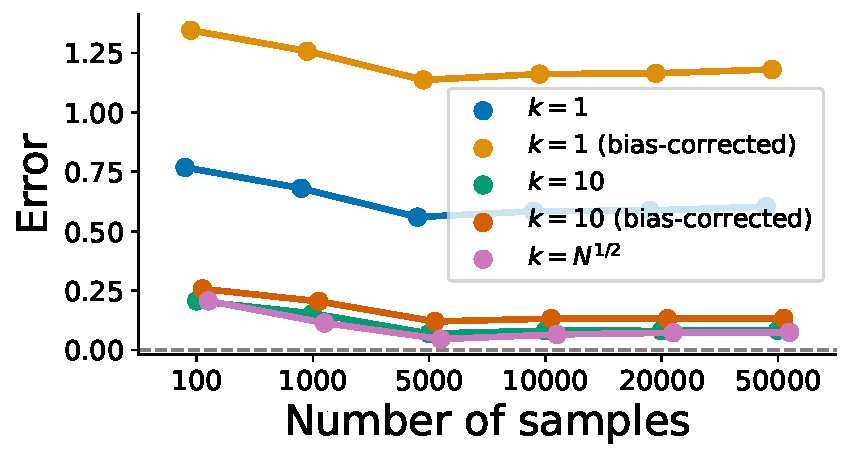
\includegraphics[width=.48\textwidth]{knnest-weak-corr-d=4-legend}}
	\subfloat[$d = 10$]{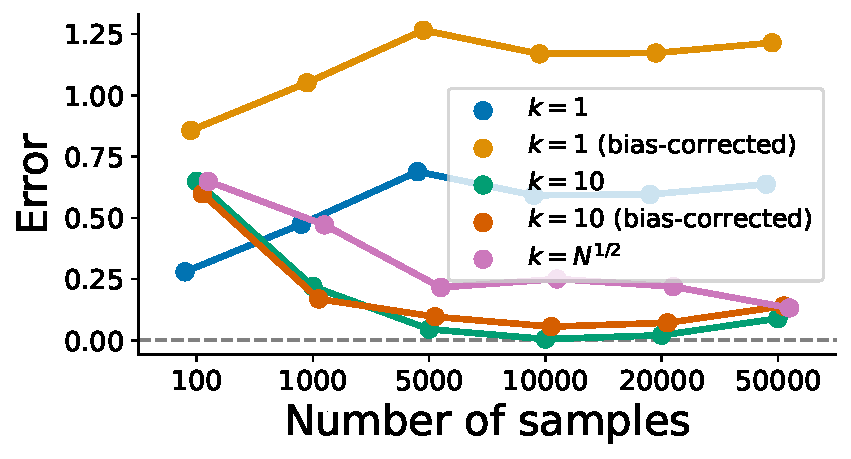
\includegraphics[width=.48\textwidth]{knnest-weak-corr-d=10-legend}}
	\\
	\subfloat[$d = 25$]{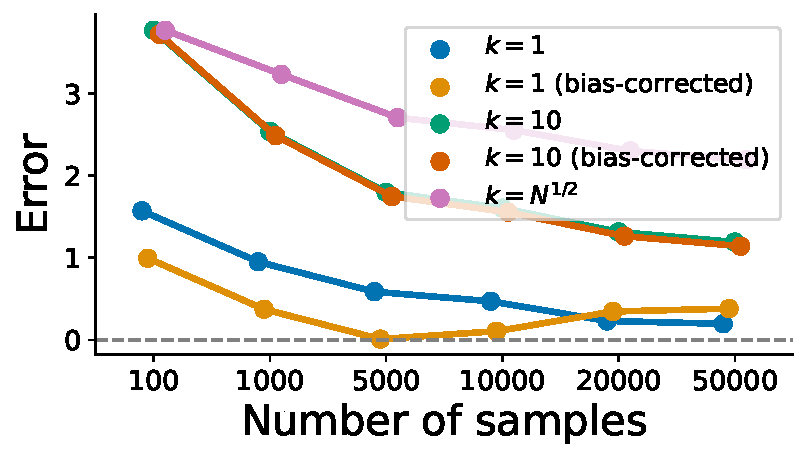
\includegraphics[width=.48\textwidth]{knnest-weak-corr-d=25-legend}}
	\subfloat[$d = 50$]{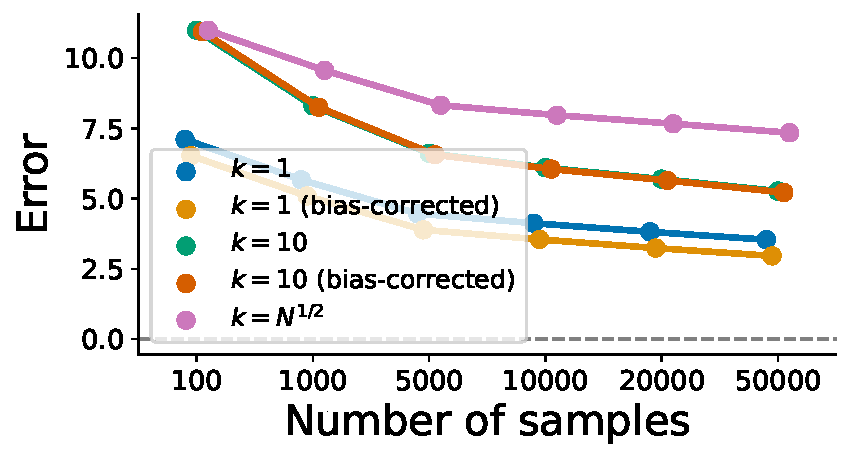
\includegraphics[width=.48\textwidth]{knnest-weak-corr-d=50-legend}}
	\caption{Absolute error against sample size for canonical $1$-nearest-neighbor estimator, canonical $10$-nearest-neighbor estimator, bias-corrected $1$-nearest-neighbor estimator, bias-corrected $10$-nearest-neighbor estimator and adaptive $k_{\numobs}$-nearest-neighbor estimator with $k_{\numobs}=\numobs^{1/2}$. Each panel corresponds with a different dimension $D\in\{4,10,25,50\}$. Gray dotted lines indicate no error.}
	\label{fig:knn-kl-est-comparison}
\end{figure}


\section{Checking \cref{assump:bounded-ratios}} \label{sec:checking-assumptions}

% We illustrate using a mixture of t-distributions and mixture of binomial distributions below.
%\begin{example}[Mixtures of t-distributions]
%\label{exa:t-dist}

\subsection{Mixture of t-distributions}
\label{appx:mixture-tdist-check}
	Consider the true data-generating distribution as a mixture of univariate t-distributions $P_{o}(\dee x)=\sum_{k = 1}^{\numcomps_{o}}\eta_{ok}F_{o}(\dee x; m_k, \tau_k, \nu)$ where the component density is 
    \[
    f_{o}(x;m,\tau, \nu) = \frac{\Gamma\left(\frac{\nu+1}{2}\right)}{\tau\sqrt{\nu \pi}\Gamma\left(\frac{\nu}{2}\right)}\left[\frac{\nu+\left(\frac{x-m}{\tau}\right)^2}{\nu}\right]^{-\left(\frac{\nu+1}{2}\right)}
    \]
    and $\Gamma(\cdot)$ is the gamma function. 
    Denote the asymptotic fitted Gaussian mixture model as $G_{\star}(\dee x) = \sum_{k=1}^{\numcomps}\eta_{\star k} F_{\star k}(\dee x)$,
    where $F_{\star k} = \distNorm(\mu_{\star k}, \sigma^2_{\star k})$. 
    %with density $f_{\star}(x; \mu, \sigma^2 )=\frac{1}{\sigma \sqrt{2\pi}}\exp\left(-\frac{1}{2}\left(\frac{x-\mu}{\sigma}\right)^2\right)$. 

    %Assume the degrees of freedom for $f_{o\ell}$ are equal for all $\ell$. 
    We want to show that $\sup_x\{ p_{\star}^{(\numcomps_{o})}(k \mid x)/p_{o}(k \mid x) \}< \infty$ when $\numcomps = \numcomps_{o}$.
	%It's easy to see $\eta_{\star k}/\eta_{ok} < \infty$. 
    Letting $\bar{\ell} = \argmax_\ell \sigma_{\star \ell}$, we have
	\begin{align}
		\sup_{x}\left\{\frac{p_{\star}^{(\numcomps_{o})}(k \mid x)}{p_{o}(k \mid x)}\right\}
		 & = \sup_{x}\left\{\frac{\eta^{(\numcomps_o)}_{\star k}f^{(\numcomps_o)}_{\star k}(x)}{g^{(\numcomps_o)}_{\star}(x)}\right\}\cdot \frac{p_{o}(x)}{\eta_{ok}f_{ok}(x)}    \\
		 & = \sup_{x}\left\{\frac{\eta^{(\numcomps_o)}_{\star k}}{\eta_{ok}} \cdot  \frac{f^{(\numcomps_o)}_{\star k}(x)}{\sum_{\ell=1}^{\numcomps_{o}}\eta^{(\numcomps_o)}_{\star \ell}f^{(\numcomps_o)}_{\star \ell}(x)} \cdot \frac{\sum_{\ell=1}^{\numcomps_{o}}\eta_{o\ell}f_{o\ell}(x)}{f_{ok}(x)}\right\} \\
         & < \frac{\eta^{(\numcomps_o)}_{\star k}\eta_{o\ell'}}{\eta_{ok}\eta^{(\numcomps_o)}_{\star \bar{\ell}}} \sup_{x} \left\{  \frac{f^{(\numcomps_o)}_{\star k}(x)}{f^{(\numcomps_o)}_{\star \bar{\ell}}(x)}\right\} \cdot  \sum_{\ell=1, \ell\ne k}^{\numcomps_o}\sup_{x}\left\{\frac{f_{o\ell}(x)}{f_{ok}(x)}\right\}. \label{eq:posterior-ratio}
	\end{align}
    Since $\sigma_{\star \bar{\ell}}$ is maximal, we can conclude that 
\begin{align}
\sup_{x} \left\{  \frac{f^{(\numcomps_o)}_{\star k}(x)}{f^{(\numcomps_o)}_{\star \bar{\ell}}(x)}\right\} = \sup_{x} \left\{ \frac{\sigma_{\star \bar{\ell}
}}{\sigma_{\star k}}\exp\left[\frac{1}{2} \left(\left(\frac{x-\mu_{\star \bar{\ell}}}{\sigma_{\star \bar{\ell}}}\right)^2 -\left(\frac{x-\mu_{\star k}}{\sigma_{\star k}}\right)^2 \right)\right] \right\} < \infty, \label{eq:sec-term}
\end{align}
and so it follows that 
\begin{align}
    \sum_{\ell=1, \ell\ne k}^{\numcomps_o}\sup_{x}\left\{\frac{f_{o\ell}(x)}{f_{ok}(x)}\right\} =  \sum_{\ell=1, \ell\ne k}^{\numcomps_o}\frac{\tau_{ok}}{\tau_{o\ell}} \sup_x \left\{ \left(\frac{\nu+\left(\frac{x-m_{o\ell}}{\tau_{o\ell}}\right)^2}{\nu+\left(\frac{x-m_{ok}}{\tau_{ok}}\right)^2}\right)^{-\left(\frac{\nu+1}{2}\right)} \right\} < \infty. \label{eq:third-term}
\end{align}
Plugging \cref{eq:sec-term,eq:third-term} back to \cref{eq:posterior-ratio} yields $\sup_x\{ p_{\star}^{(\numcomps_{o})}(k \mid x)/p_{o}(k \mid x) \}< \infty$ .


%The last term in \cref{eq:posterior-ratio} is the ratio between normal and t-distribution densities. For simplicity, we ignore the $k$-dependency in the densities and write
	% \begin{align}
	% 	\sup_x \frac{f(x; \mu,\sigma^2)}{f_{ok}(x; m, \tau, \nu)} = \frac{\tau}{\sigma}\cdot\frac{\Gamma\left(\frac{\nu}{2}\right)}{\Gamma\left(\frac{\nu+1}{2}\right)}\cdot\sqrt{\frac{\nu}{2}}\cdot \sup_x  \exp\left(-\frac{1}{2}\left(\frac{x-\mu}{\sigma}\right)^2\right) \cdot \left[\frac{\nu+\left(\frac{x-m}{\tau}\right)^2}{\nu}\right]^{\left(\frac{\nu+1}{2}\right)}. \label{eq:normal-t-ratio}
	% \end{align}
	% Observe that $\lim\limits_{\nu\rightarrow\infty}p_{o}(x; m, \tau, \nu) = f(x; m, \tau^2)$. The ratio in \cref{eq:normal-t-ratio} converges to $0$ for $\nu$ small and $|x|$ large.\PROBLEM{TODO(Jiawei): we want to be able to say that the $\sup$ over $x$ of the ratio of densities is finite.}

	% On the other hand, consider the ratio of mixture weights
	% \begin{align}
	% 	\frac{\eta^{(\numcomps_o)}_{\star k}}{\eta_{o}} = \frac{\int p^{(\numcomps_{o})}_{\star}(k\mid y)P_{o}(\dee y)}{\int p_{o}(k\mid y)P_{o}(\dee y)}
	% \end{align}
%\end{example}

%\begin{example}[Mixtures of negative binomial distributions]
\subsection{Mixture of bounded discrete distributions}

Suppose data are generated from a mixture of discrete distributions $P_{o}(\dee x)=\sum_{k = 1}^{\numcomps_{o}}\eta_{ok}F_{ok}(\dee x)$ with a finite support $\mathcal{X}$ for all $F_{ok}$. 
Denote the asymptotic fitted Poisson mixture model as $G_{\star}(\dee x) = \sum_{k=1}^{\numcomps}\eta_{\star k} F_{\star k}(\dee x)$, 
where $F_{\star k} = \distPoiss(\lambda_{\star k})$.
%$f_{\star}(x; \lambda)=\frac{\lambda^x e^{-\lambda}}{x!}$. 

To show $\sup_{x \in \mathcal{X}} \{p_{\star}^{(\numcomps_{o})}(k \mid x)/p_{o}(k \mid x)\} < \infty$ when $\numcomps = \numcomps_{o}$, we only need to show $\sup_{x} \left\{  f^{(\numcomps_o)}_{\star k}(x)/f^{(\numcomps_o)}_{\star \bar{\ell}(x)}\right\}<\infty$ and $ \sum_{\ell=1, \ell\ne k}^{\numcomps_o}\sup_{x}\left\{f_{o\ell}(x)/f_{ok}(x)\right\} < \infty$ according to \cref{eq:posterior-ratio}. Define $\bar{\ell} = \argmax_\ell \lambda_{\star \ell}$.  
Since $\lambda_{\star \bar{\ell}}$ is maximal, we can conclude that
    \begin{align}
\sup_{x} \left\{  \frac{f^{(\numcomps_o)}_{\star k}(x)}{f^{(\numcomps_o)}_{\star \bar{\ell}}(x)}\right\} = \sup_{x} \left\{ \left(\frac{\lambda_{\star k}}{\lambda_{\star \bar{\ell}}}\right)^x e^{-(\lambda_{\star \bar{\ell}} - \lambda_{\star k} )}\right\} < \infty. \label{eq:negbin-sec-term}
\end{align}
On the other hand, it follows by the finite support for $F_{ok}$ that 
\begin{align}
    \sum_{\ell=1, \ell\ne k}^{\numcomps_o}\sup_{x\in\mathcal{X}}\left\{\frac{f_{o\ell}(x)}{f_{ok}(x)}\right\} < \infty. \label{eq:neg-bin-third-term}
\end{align}
Combining \cref{eq:negbin-sec-term,eq:neg-bin-third-term} yields $\sup_x\{ p_{\star}^{(\numcomps_{o})}(k \mid x)/p_{o}(k \mid x) \}< \infty$.
%\end{example}

\section{Checking \cref{assump:sample_approx_able}}\label{sec:sample_approx_able_example}

We show that \cref{assump:sample_approx_able} holds for both the PMF models used for the experiments in \cref{sec:experiments}. 
% Although the assumption is stated in terms of the full sequence $y_{1:K}$, 
It is sufficient to verify the assumption for a single element $y_{nk}$ since the variance and integrability conditions can often be checked component-wise.
Hence, we drop the dependence on $n$ and $k$ in our notation. 

\subsection{Poisson PMF}

Consider the Poisson model with  $y \sim \distPoiss(\lambda)$ and $\lambda = W h$.
For convenience, we assume $h \sim \distGamma(\alpha, \beta)$.
%so
To compute the first and second moments of 
\[
  P(y\mid h) = \frac{(W h)^{y} e^{-W h}}{y!},
\]
we will use the identity
$\Gamma(z) = \int_0^\infty t^{z-1} e^{-t} \, \d t$ and integration by substitution.
For the first moment we have 
\begin{align}
\mathbb{E}_{h}\bigl[P(y\mid h)\bigr]
  &= \int_{0}^{\infty} \frac{(W h)^{y} e^{-W h}}{y!}
     \;\frac{\beta^{\alpha}}{\Gamma(\alpha)} h^{\alpha-1} e^{-\beta h} \, \mathrm{d}h\\[6pt]
  &= \frac{W^{y} \beta^{\alpha}}{y!\,\Gamma(\alpha)}
     \int_{0}^{\infty} h^{y+\alpha-1} e^{-(W+\beta)h} \, \mathrm{d}h\\[6pt]
  &= \frac{W^{y} \beta^{\alpha}\,\Gamma(y+\alpha)}{y!\,\Gamma(\alpha)(W+\beta)^{y+\alpha}},
\end{align}
while the second moment is 
\begin{align}
\mathbb{E}_{h}\bigl[P^{2}(y\mid h)\bigr]
  &= \int_{0}^{\infty} \frac{(W h)^{2y} e^{-2 W h}}{(y!)^{2}}
     \;\frac{\beta^{\alpha}}{\Gamma(\alpha)} h^{\alpha-1} e^{-\beta h} \, \mathrm{d}h\\[6pt]
  &= \frac{W^{2y} \beta^{\alpha}}{\Gamma(\alpha)(y!)^{2}}
     \int_{0}^{\infty} h^{2y+\alpha-1} e^{-(2W+\beta)h} \, \mathrm{d}h\\[6pt]
  &= \frac{W^{2y} \beta^{\alpha}\, \Gamma(2y+\alpha)}{\Gamma(\alpha)(y!)^{2}(2W+\beta)^{2y+\alpha}}.
\end{align}
% 
Taking the ratio of the second to the first moment, define 
\[
  C(y) = \frac{\mathbb{E}_{h}[P^{2}(y\mid h)]}{\mathbb{E}_{h}[P(y\mid h)]}
         = \frac{W^{y} \, \Gamma(2y+\alpha)}{y!\,\Gamma(y+\alpha)}
           \left(\frac{W+\beta}{2W+\beta}\right)^{y+\alpha}
           \cdot\left(\frac{1}{2W+\beta}\right)^{y},
\]
which is continuous and finite for all $y \in \nats$. 
Now, using Stirling's approximation
$ \Gamma(z) \sim \sqrt{2\pi}\, z^{z-1/2} e^{-z},$ we have
\begin{align}
    \frac{\Gamma(2y+\alpha)}{y!\,\Gamma(y+\alpha)} &\sim
    \frac{(2y)^{2y+\alpha-1/2} e^{-2y}}{\sqrt{2\pi}\,y^{y+\alpha-1/2} e^{-y}\cdot \sqrt{2\pi}\,y^{y+1/2} e^{-y}}
    \sim \frac{2^{2y+\alpha}}{\sqrt{\pi y}}.
\end{align}
Substituting into $C(y)$ yields
\begin{align}
C(y)
 &\sim \frac{W^{y}}{\sqrt{\pi y}}
        \left(\frac{W+\beta}{2W+\beta}\right)^{\alpha}
        \left(\frac{W+\beta}{2W+\beta}\right)^{y}
        \left(\frac{1}{2W+\beta}\right)^{y}
        2^{2y}\\
 &\sim \frac{1}{\sqrt{\pi y}}
        \left(\frac{W+\beta}{2W+\beta}\right)^{\alpha}
        \left(\frac{2^2W(W+\beta)}{(2W+\beta)^2}\right)^{y}\\
 &\sim \frac{1}{\sqrt{\pi y}}
        \left(\frac{4W^2+4W\beta}{4W^2+\beta^2+4W\beta}\right)^{y}.      
\end{align}
Because $0<\frac{4W^2+4W\beta}{4W^2+\beta^2+4W\beta} < 1$, the ratio $C(y)$ decays exponentially as $y \to \infty$, 
hence $\sum_{y=0}^{\infty} C(y)  <\infty$.

\subsection{Gaussian PMF}

Consider the Gaussian setting $y \sim \mathcal{N}(\phi h, \sigma^2)$
and, following common practice, we let $h \sim \mathcal{N}(\mu, \tau^2)$. 
To compute the moments of $p(y \mid h)$, we integrate over the latent variable $h$ by combining the terms in the exponential, completing the square, and using the Gaussian integral identity
$\int_{-\infty}^{\infty} e^{-(a x^2 + b x + c)} \, \dee x = \sqrt{\frac{\pi}{a}} e^{\frac{b^2}{4a} - c}.$ 
The first moment is 
% 
\begin{align}
\mathbb{E}_h [p(y \mid h)] 
&= \int_{-\infty}^{\infty} \frac{1}{\sqrt{2\pi\sigma^2}} \exp\left(-\frac{(y - \phi h)^2}{2\sigma^2} \right)
\cdot \frac{1}{\sqrt{2\pi\tau^2}} \exp\left(-\frac{(h - \mu)^2}{2\tau^2} \right) \, dh \\
&\propto \exp\left\{ -\frac{(y - \phi \mu)^2}{2(\phi^2 \tau^2 + \sigma^2)} \right\},
\end{align}
while the second moment is 
% also the moment
\begin{align}
\mathbb{E}_h [p(y \mid h)^2] 
&= \int_{-\infty}^{\infty} \left( \frac{1}{\sqrt{2\pi\sigma^2}} \exp\left(-\frac{(y - \phi h)^2}{2\sigma^2} \right) \right)^2
\cdot \frac{1}{\sqrt{2\pi\tau^2}} \exp\left(-\frac{(h - \mu)^2}{2\tau^2} \right) \, dh \\
&\propto \exp\left\{ -\frac{(y - \phi \mu)^2}{2(\phi^2 \tau^2 + \frac{1}{2}\sigma^2)} \right\}.
\end{align}
Therefore, up to a multiplicative constant, the ratio of moments is 
\begin{align}
    C(y) 
    &= \frac{\mathbb{E}_{h}[P^{2}(y\mid h)]}{\mathbb{E}_{h}[P(y\mid h)]} \\
    &\propto \frac{ \exp\left\{ -\frac{(y - \phi \mu)^2}{2(\phi^2 \tau^2 + \frac{1}{2}\sigma^2)} \right\} }{ \exp\left\{ -\frac{(y - \phi \mu)^2}{2(\phi^2 \tau^2 + \sigma^2)} \right\} }\\
    % &= \exp\left\{ -\frac{(y - \phi \mu)^2}{2(\phi^2 \tau^2 + \frac{1}{2}\sigma^2)} + \frac{(y - \phi \mu)^2}{2(\phi^2 \tau^2 + \sigma^2)} \right\} \\
    &= \exp\left\{ -(y - \phi \mu)^2 \left( \frac{1}{2(\phi^2 \tau^2 + \frac{1}{2}\sigma^2)} - \frac{1}{2(\phi^2 \tau^2 + \sigma^2)} \right) \right\}.
\end{align}
Since $\frac{1}{2(\phi^2 \tau^2 + \frac{1}{2}\sigma^2)} > \frac{1}{2(\phi^2 \tau^2 + \sigma^2)}$, 
we get $C(y) \propto \exp\left\{ -a (y - \phi \mu)^2 \right\}$ for some $a > 0$. Therefore,
$C(y)$ decays exponentially as $y \to \infty$ and hence $\int C(y)\d y <\infty$.  


\section{Limitations of Coarsening}

\PROBLEM{XXX: maybe remove?}

The following toy example illustrates how coarsening and the Bayesian information criterion can overfit even in scenarios with only a modest degree of misspecification.
%\begin{example}[Illustration: Overfitting the Number of Mixture Model Components]
	% Finding $\numcomps_{o}$ can be challenging for standard model selection approaches given the presence of model misspecification \citep{Cai:2021,Guha:2021,Fruhwurth:2006,Miller:2019}.
	% Specifically, as the number of observations increases, model selection criteria tend to create additional clusters to compensate for the model--data mismatch and thus overestimates
	% $\numcomps_{o}$.

	%do not always provide robust model selection consistency.
	We generate data from a mixture of $\numcomps_{o} = 2$ skew normal distributions but fit the data using a Gaussian mixture.
	The level of misspecification is controlled by the skewness parameter of each skew normal component in the true generative distribution $P_{o}$.
	We consider the following scenarios: two equal-sized clusters with the same level of misspecification (denoted \texttt{same})
	and two equal-sized clusters with different levels of misspecification (denoted \texttt{different}).
	See \cref{sec:high-dim-simulation} for further details about the experimental set-up.
	%\begin{enumerate}[(i)]
	%	%	\item \label{eg:s1} two equal-sized clusters with no misspecification;
	%	\item \label{eg:s2}two equal-sized clusters with the same level of misspecification;
	%	\item \label{eg:s3} two equal-sized clusters with different levels of misspecification.
	%	%	\item \label{eg:s4} two different-sized clusters with same level of misspecification.
	%\end{enumerate}
	As shown in the first row of \cref{fig:motivate-comparison}, in both scenarios using expectation--maximization (EM)
	with the Bayesian information criterion (BIC) results in estimating $\numcomps \gg \numcomps_{o}$
	to capture the skewness of each component.
	As shown in the second row of \cref{fig:motivate-comparison},
	the coarsened posterior performs well in the \texttt{same} case but overfits the cluster with a larger degree of misspecification in the \texttt{different} scenario.
	% its limitations become evident when the degree of misspecification differs significantly between components.
	% In the , the coarsened posterior overfits the cluster with a larger degree of misspecification.
	%the coarsened posterior \citep{Miller:2019}, and EM with our proposed model selection criterion.
	%Depending on the comparable sizes and levels of misspecification between components, the candidate inferences perform differently. We discuss the setup parameters with more detail in  
	% % as number of observations increases. 
	% %Such overfitting phenomena raise severe concern about existing inference on the identification about the correct number of latent types with finite mixture models, when model is ill-defined.
	% %\end{example}
	% While the coarsened posterior  performs well in the \texttt{same} case,
	% some limitations become evident when the degree of misspecification differs significantly between components.
	% In the \texttt{different} scenario, the coarsened posterior overfits the cluster with a larger degree of misspecification.
	% %This limitation arises from applying robustness at the overall model level.
	% %, which leads to a roughly even distribution of this robustness across each component. 
	% %In \cref{sec:simulation-gauss}, we also that the coarsened posterior generally fails to capture $\numcomps_{o}$ when components are of relatively different degrees of misspecification scaled by component size. =	
%\end{example}


\begin{figure}[tp]
	\centering
	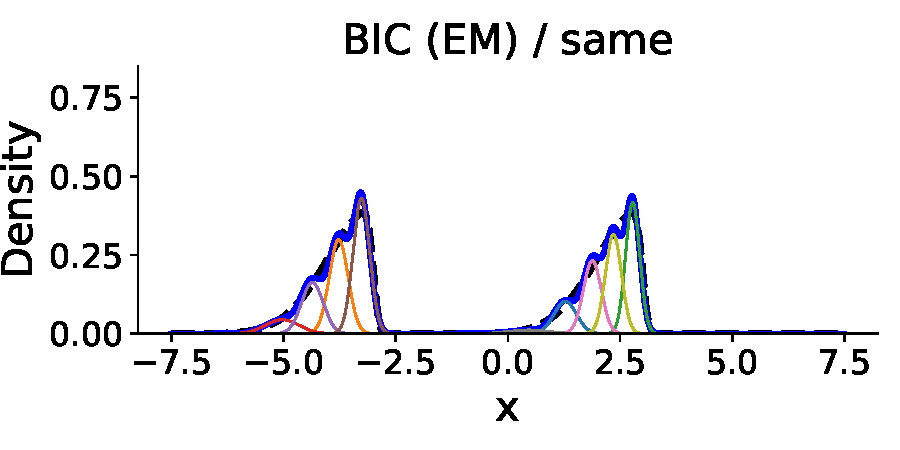
\includegraphics[width=.48\textwidth]{em-pdfs-n=5000-close-False-rsize-equal-rmis-equal}
	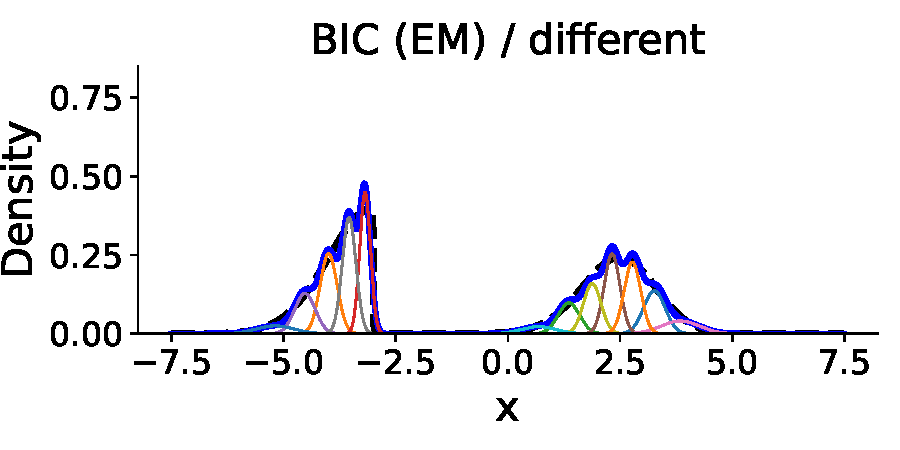
\includegraphics[width=.48\textwidth]{em-pdfs-n=10000-close-False-rsize-equal-rmis-bbig-small}\\
	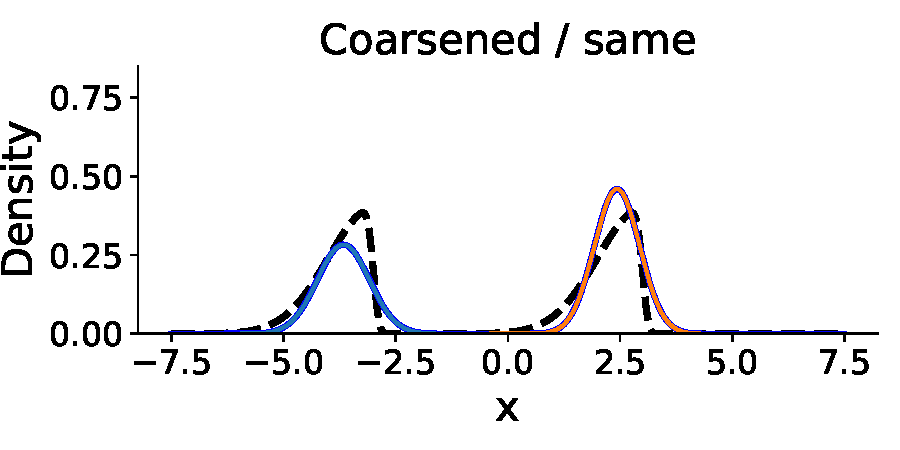
\includegraphics[width=.48\textwidth]{skewnorm-coarsen-pdfs-n=5000-close-False-rsize-equal-rmis-equal}
	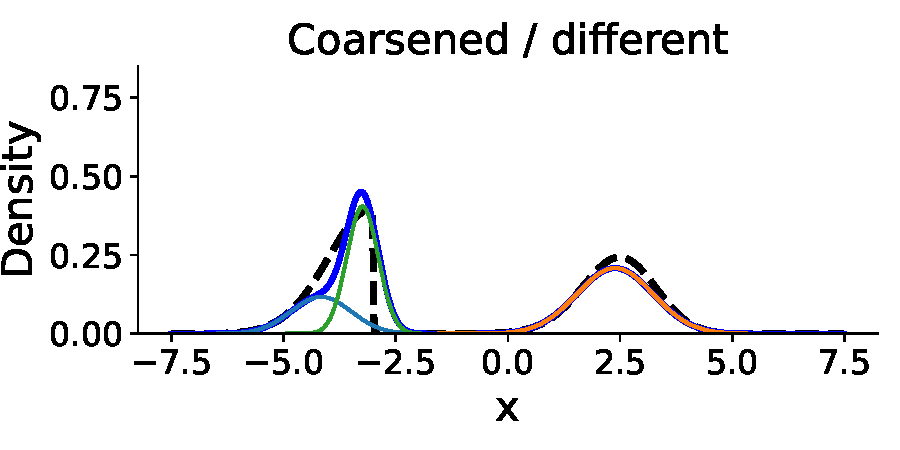
\includegraphics[width=.48\textwidth]{skewnorm-coarsen-pdfs-n=10000-close-False-rsize-equal-rmis-bbig-small}\\
	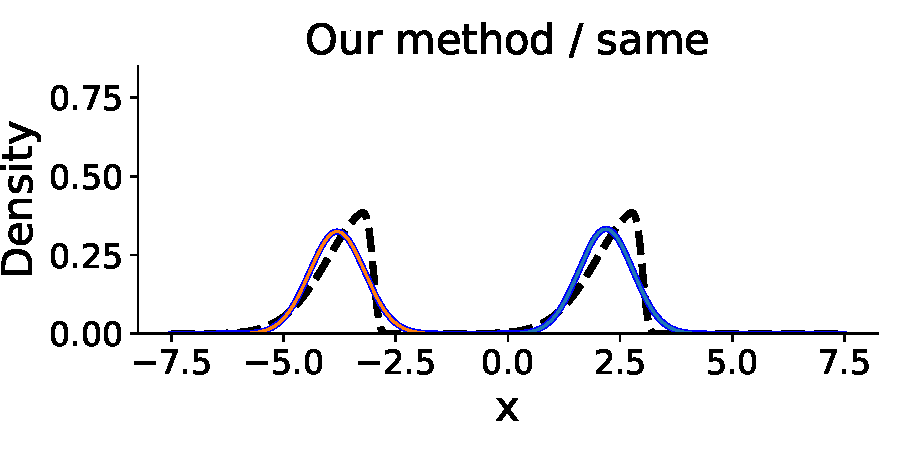
\includegraphics[width=.48\textwidth]{skewnorm-stare-pdfs-n=5000-close-False-rsize-equal-rmis-equal}
	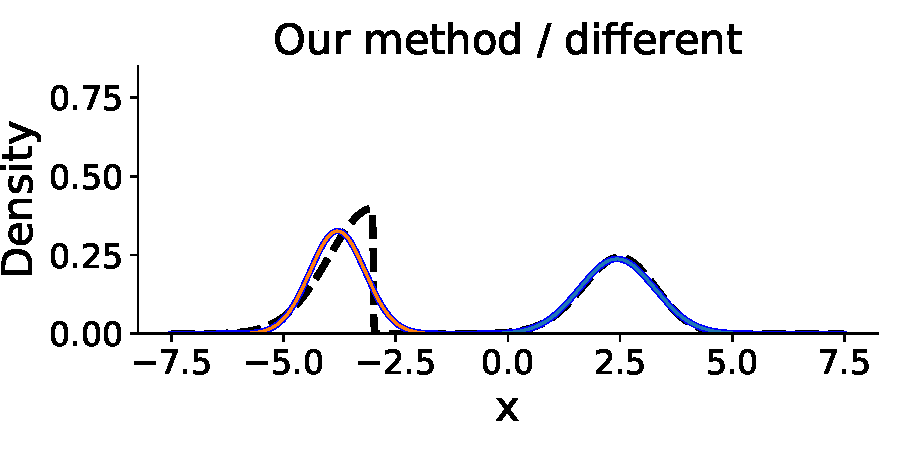
\includegraphics[width=.48\textwidth]{skewnorm-stare-pdfs-n=10000-close-False-rsize-equal-rmis-bbig-small}
	\caption{
		For the mixture of skew-normals example from \cref{sec:intro},
		each panel shows the density of $P_{o}$ (dashed lines) and the densities of the fitted Gaussian mixture model and each
		component distribution (solid lines) using $\numobs = 10\,000$ observations.
		The ``same'' and ``different'' scenarios describes the relative degree of misspecification of the two components.
		Results are given for three approaches:
		expectation--maximization with the Bayesian information criterion (first row),
		the coarsened posterior (second row),
		and our robust model selection method (third row).}
	\label{fig:motivate-comparison}
\end{figure}


\section{Additional Calibration Figures}

\subsection{Simulation Study}
\label{appx:simulation-gauss}

The coarsened posterior requires calibration of the hyperparameter $\alpha$, which determines the degree of misspecification.
We select $\alpha$ using the \emph{elbow method} proposed by \citet{Miller:2019}.
In this section, we include all calibration figures for the coarsened posterior following the code provided by \citet{Miller:2019}.

As shown in \cref{fig:coarsen-calibration}, we set $\alpha$ based on the turning point where we see no significant increase
in the log-likelihood if $\alpha$ increases further.
Using these values for $\alpha$, we can see for all cases except the \texttt{small-large} case, the coarsened posterior consistently estimates the number of clusters (after removing mini clusters with size $<2\%$) as $\widehat{\numcomps} = 3 > \numcomps_{o} = 2$.

\begin{figure}[tp]
	\centering
	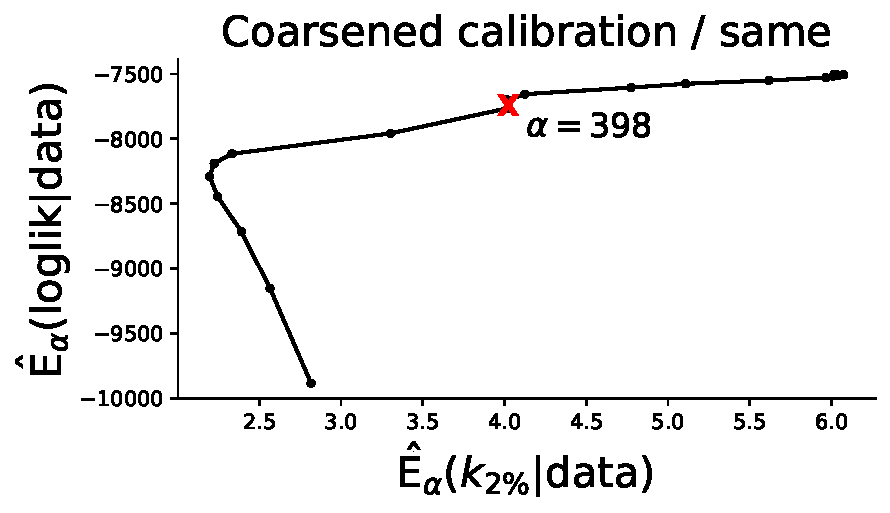
\includegraphics[width=.48\textwidth]{skewnorm-coarsen-calibration-n=5000-close-False-rsize-equal-rmis-equal}
	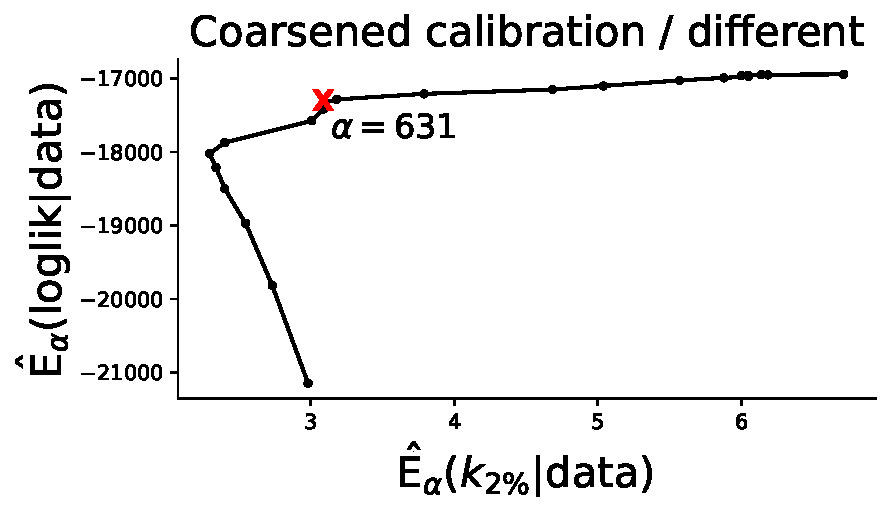
\includegraphics[width=.48\textwidth]{skewnorm-coarsen-calibration-n=10000-close-False-rsize-equal-rmis-bbig-small}\\
	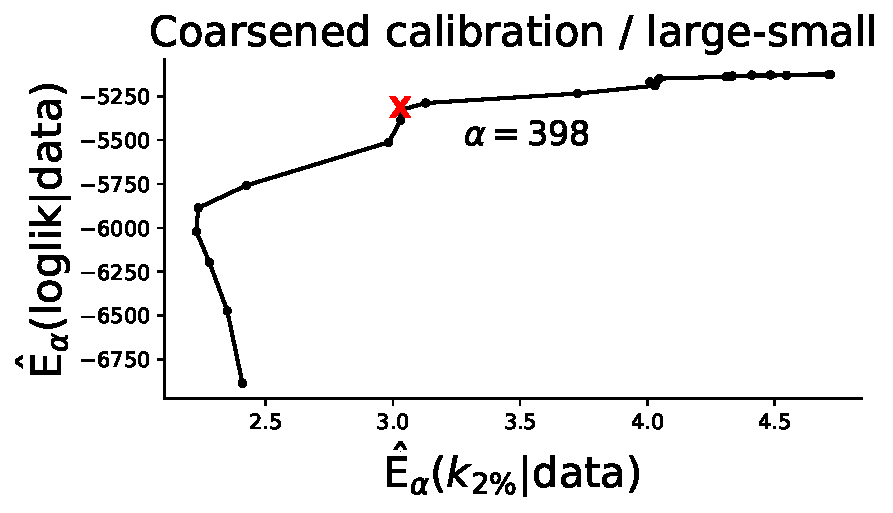
\includegraphics[width=.48\textwidth]{skewnorm-coarsen-calibration-n=5000-close-False-rsize-big-small-rmis-big-small}
	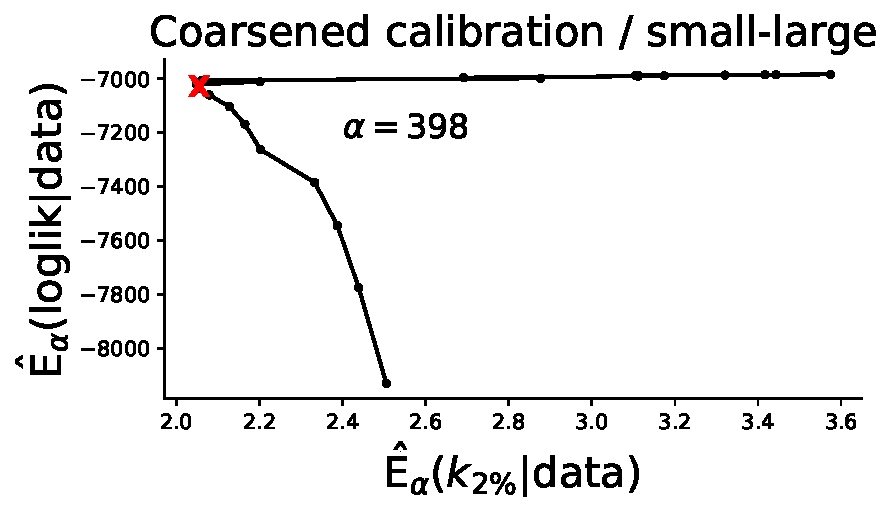
\includegraphics[width=.48\textwidth]{skewnorm-coarsen-calibration-n=5000-close-False-rsize-big-small-rmis-small-big}\\
	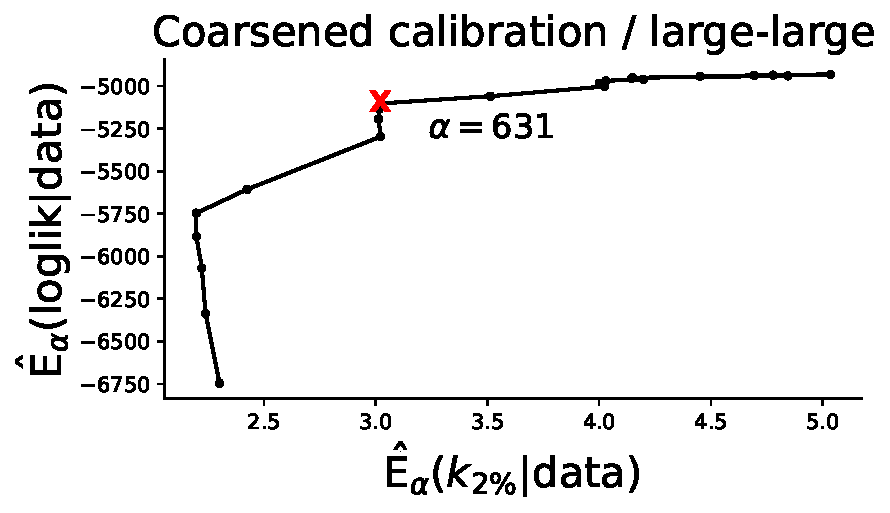
\includegraphics[width=.48\textwidth]{skewnorm-coarsen-calibration-n=5000-close-False-rsize-big-small-rmis-equal}
	\caption{For the mixture of skew normals experiments from \cref{sec:intro,sec:high-dim-simulation}, each panel shows the expected log-likelihood $\widehat{E}_{\alpha}(\mathrm{loglik}\mid \mathrm{data})$ against the expected number of clusters which excludes tiny clusters of size less that $2\%$ of whole dataset denoted as $\widehat{E}_{\alpha}(k_{2\%}\mid \mathrm{data})$.
		We select $\alpha$ as the elbow point in the plots.}
	\label{fig:coarsen-calibration}
\end{figure}

\subsection{Flow Cytometry Data}
\label{appx:flow-cytometry}

In this section, we include loss and F-measure plots of our model selection method on all test datasets 7--12.
See \citet[Section 5.2]{Miller:2019} for a discussion of the exact calibration procedure for the coarsened posterior.
% on flow cytometry datasets and recommend users to refer to .

Recall that to calibrate $\rho$, we select $\rho$ that optimizes the F-measure across first $6$ datasets.
To incorporate this prior knowledge on test datasets, we suggests selecting the value of $\numcomps$
that has has stable penalized loss and is closest to the optimal $\rho$.
We compare our selection $\widehat{\numcomps}$ with the ground truth $\numcomps_o$ labeled by experts.
For each dataset, there is always one cluster labeled as unknown due to some unclear information for cells.
With automatic clustering algorithm, it is natural for the algorithm to identify those unlabeled points and assign them to other clusters, which results in $\numcomps_o-1$ clusters.
So we treat both $\numcomps_o$ and $\numcomps_o-1$ as ground truth in our analysis.
As shown in \cref{fig:GvHD,fig:GvHD2}, our selection method results in highest F-measure for datasets 8--12.
Dataset 7 is challenging and even the ground truth does not produce a large F-measure.




\begin{figure}[tp]
	\centering
	\subfloat[Data 7]{\label{fig:data7}
		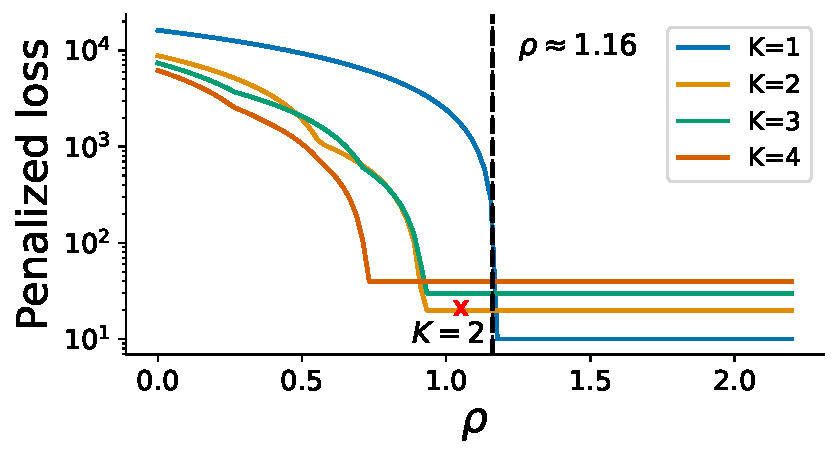
\includegraphics[width=.48\textwidth]{GvHD7-loss-plot-legend}
		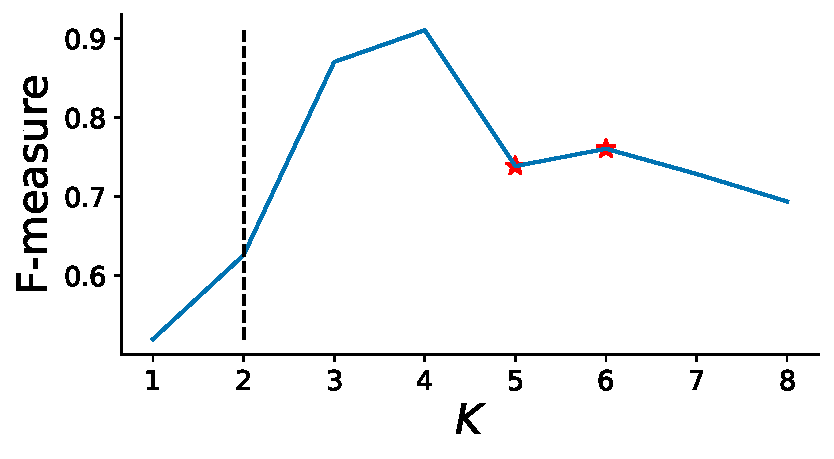
\includegraphics[width=.48\textwidth]{GvHD7-fmeasure-plot}}	\\
	\subfloat[Data 8]{\label{fig:data8}
		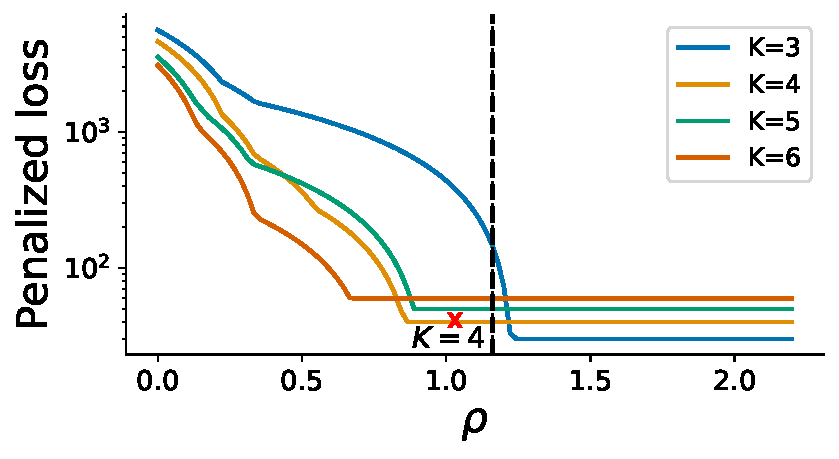
\includegraphics[width=.48\textwidth]{GvHD8-loss-plot-legend}
		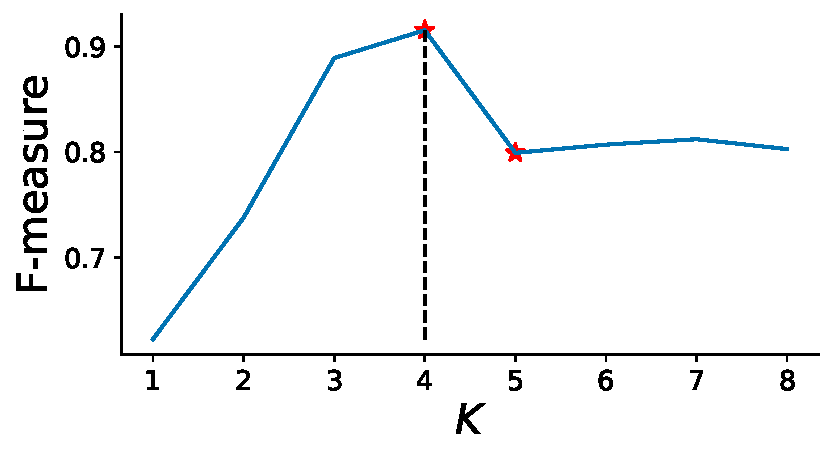
\includegraphics[width=.48\textwidth]{GvHD8-fmeasure-plot}}	\\
	\subfloat[Data 9]{\label{fig:data9}
		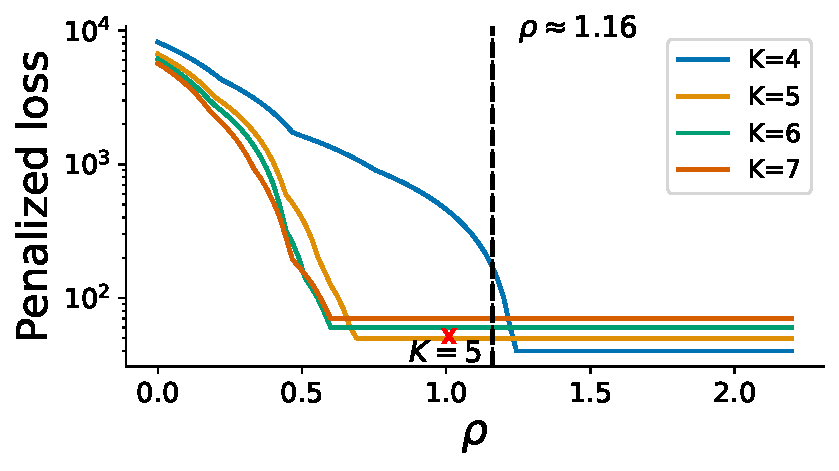
\includegraphics[width=.48\textwidth]{GvHD9-loss-plot-legend}
		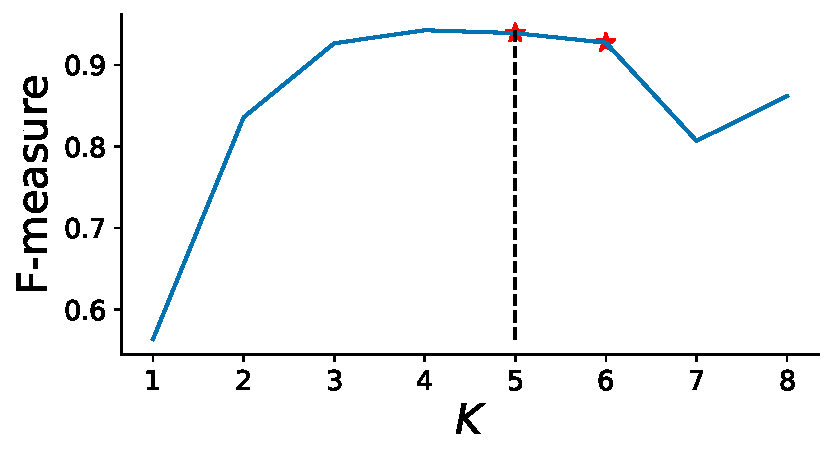
\includegraphics[width=.48\textwidth]{GvHD9-fmeasure-plot}}
	\caption{Calibration and F-measure plots for test datasets 7--9 in flow cytometry experiments. \textbf{Left}: The black dashed lines indicate the optimal $\rho$ calibrated on training datasets 1--6. The cross mark indicates the selection for number of clusters. \textbf{Right}: F-measure against the number of clusters. The dashed line shows the number of clusters selected by \methodname and the red star indicates the ground truth $\numcomps_{o}$.}
	\label{fig:GvHD}
\end{figure}


\begin{figure}[tp]
	\centering
	\subfloat[Data 10]{\label{fig:data10}
		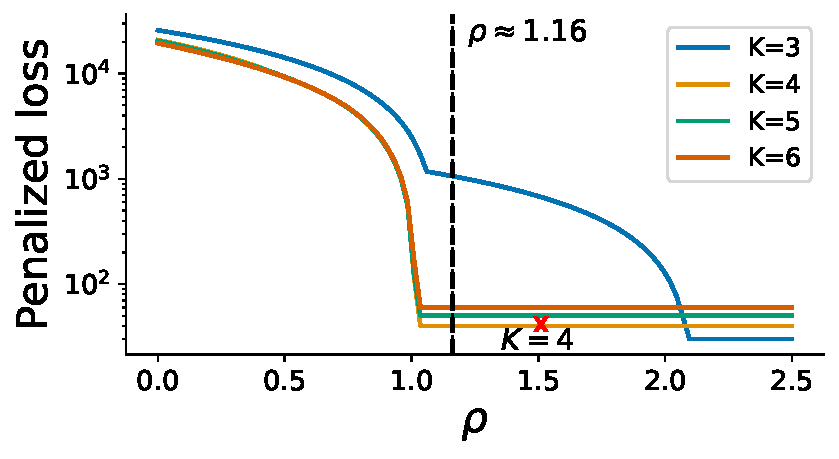
\includegraphics[width=.48\textwidth]{GvHD10-loss-plot-legend}
		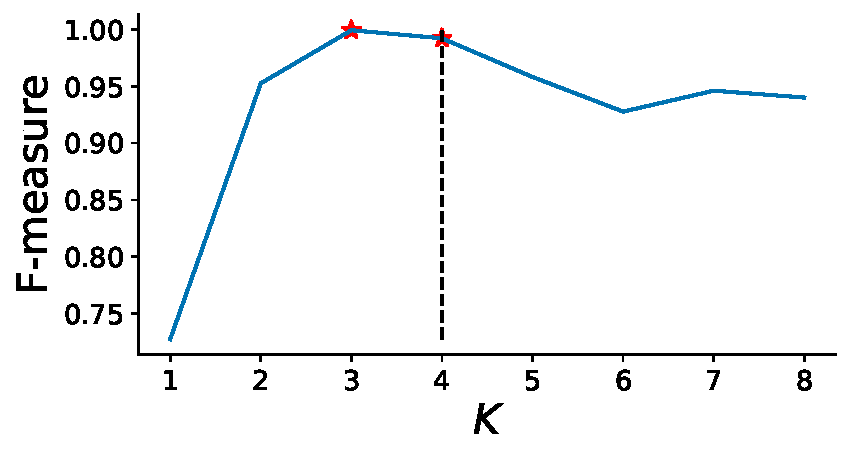
\includegraphics[width=.48\textwidth]{GvHD10-fmeasure-plot}}	\\
	\subfloat[Data 11]{\label{fig:data11}
		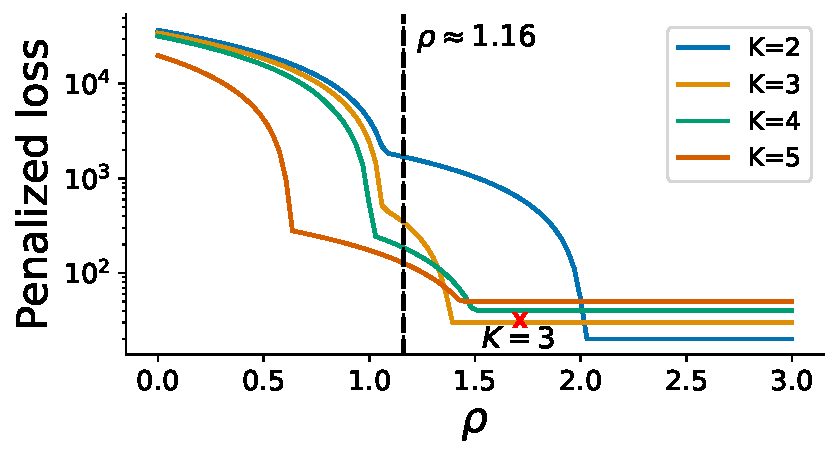
\includegraphics[width=.48\textwidth]{GvHD11-loss-plot-legend}
		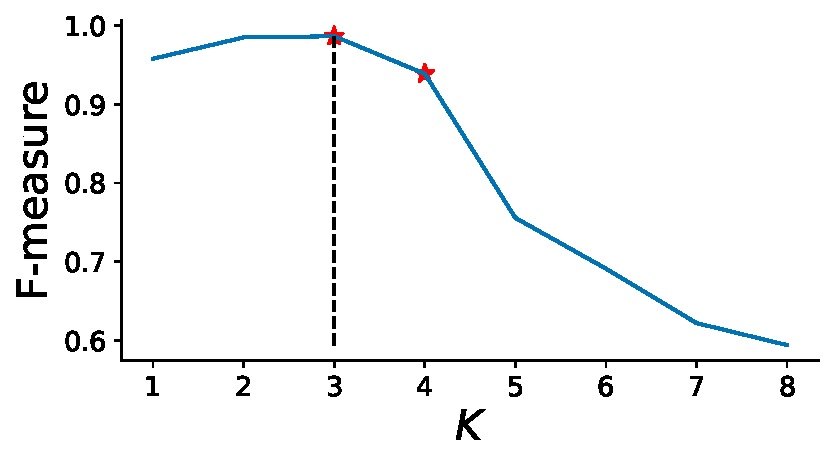
\includegraphics[width=.48\textwidth]{GvHD11-fmeasure-plot}}	\\
	\subfloat[Data 12]{\label{fig:data12}
		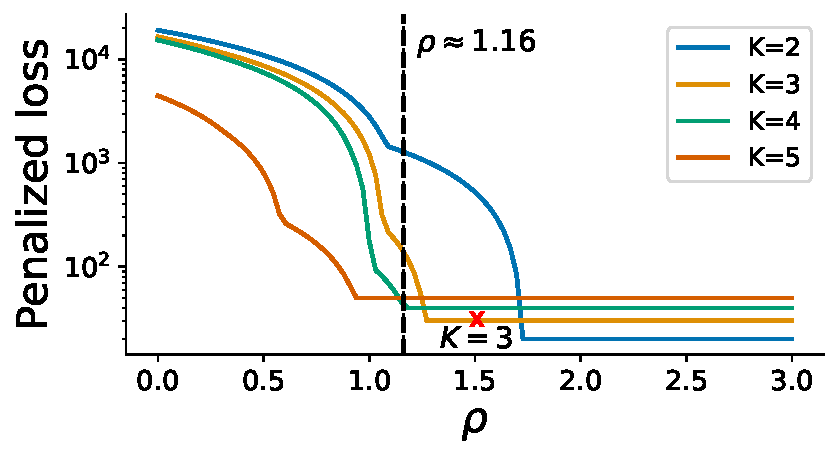
\includegraphics[width=.48\textwidth]{GvHD12-loss-plot-legend}
		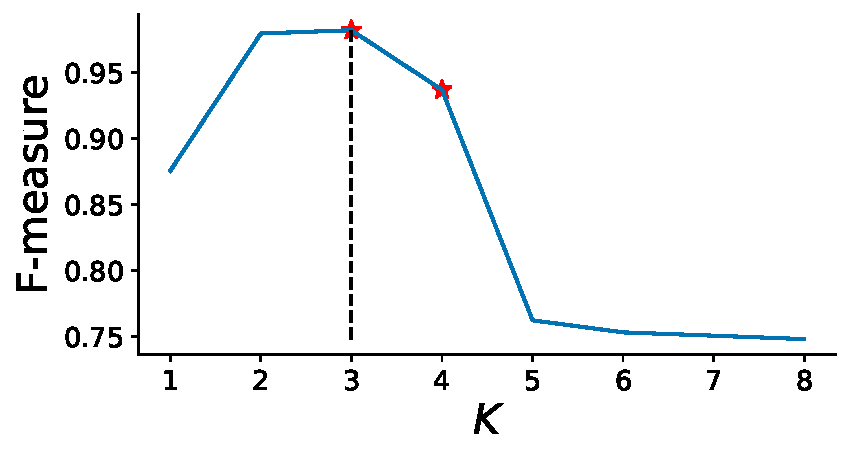
\includegraphics[width=.48\textwidth]{GvHD12-fmeasure-plot}}
	\caption{Calibration and F-measure plots for test datasets $10-12$ in flow cytometry experiments. See caption for \cref{fig:GvHD} for details}
	\label{fig:GvHD2}
\end{figure}




\begin{figure}[tp]
	\centering
	\subfloat[Data 7, $\numcomps=8$]{\label{fig:data7-loss}
		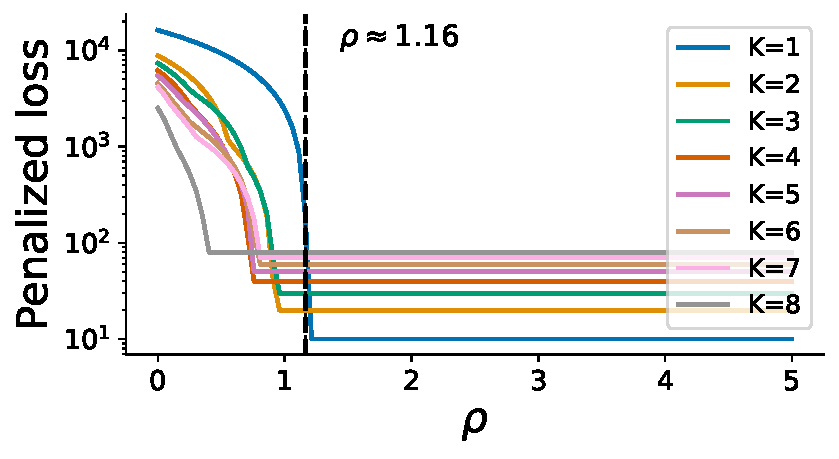
\includegraphics[width=.48\textwidth]{GvHD7-all-loss-plot-legend}}
	\subfloat[Data 8, $\numcomps=7$]{\label{fig:data8-loss}
		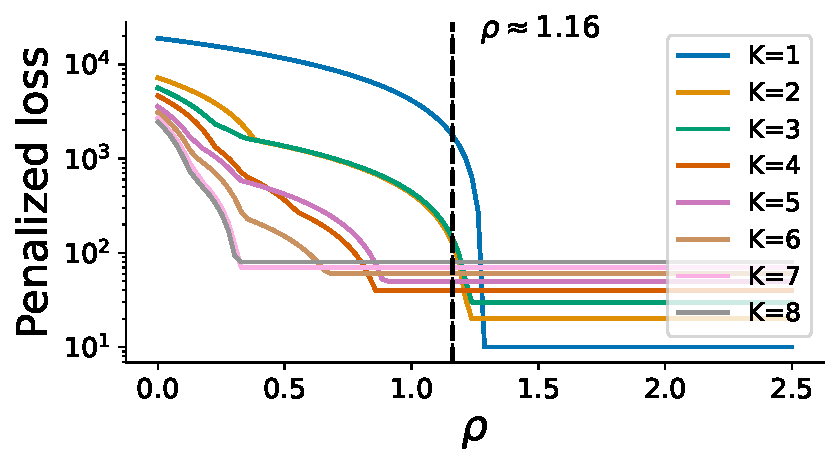
\includegraphics[width=.48\textwidth]{GvHD8-all-loss-plot-legend}}\\
	\subfloat[Data 9, $\numcomps=5$]{\label{fig:data9-loss}
		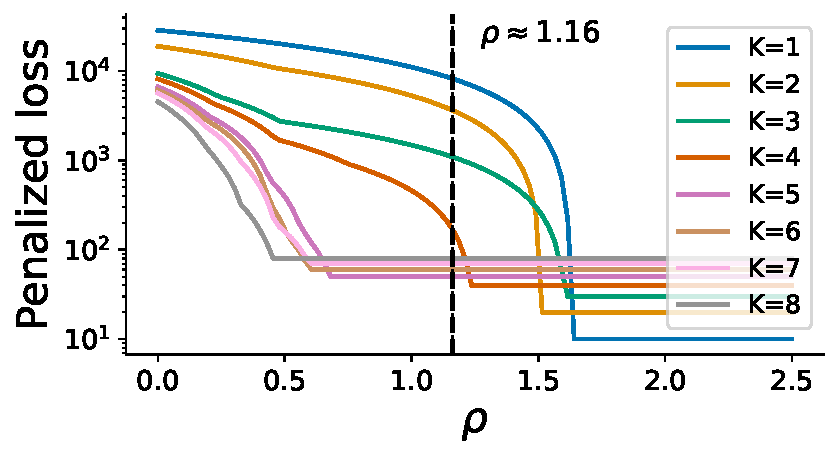
\includegraphics[width=.48\textwidth]{GvHD9-all-loss-plot-legend}}
	\subfloat[Data 10, $\numcomps=4$]{\label{fig:data10-loss}
		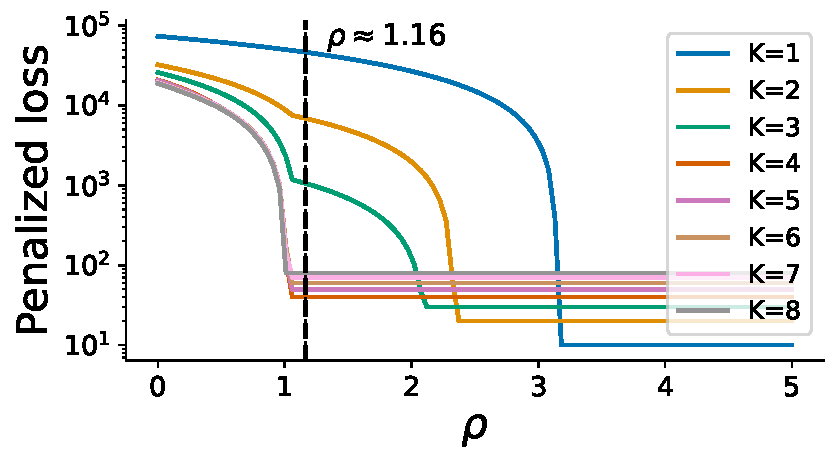
\includegraphics[width=.48\textwidth]{GvHD10-all-loss-plot-legend}}\\
	\subfloat[Data 11, $\numcomps=3$]{\label{fig:data11-loss}
		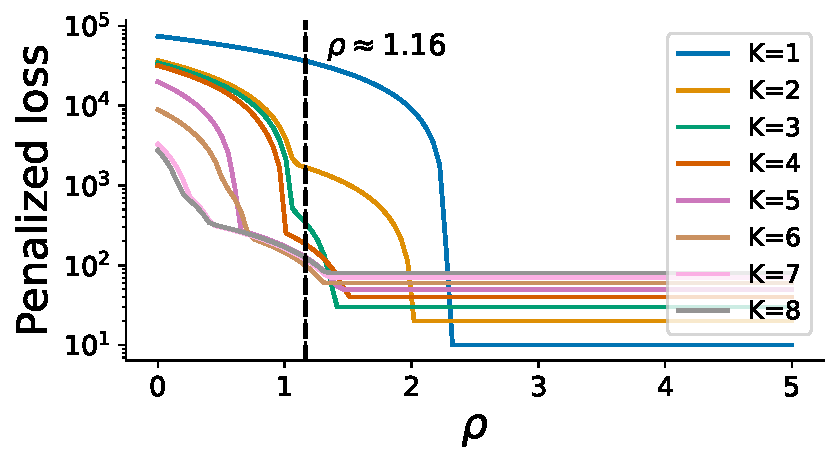
\includegraphics[width=.48\textwidth]{GvHD11-all-loss-plot-legend}}
	\subfloat[Data 12, $\numcomps=3$]{\label{fig:data12-loss}
		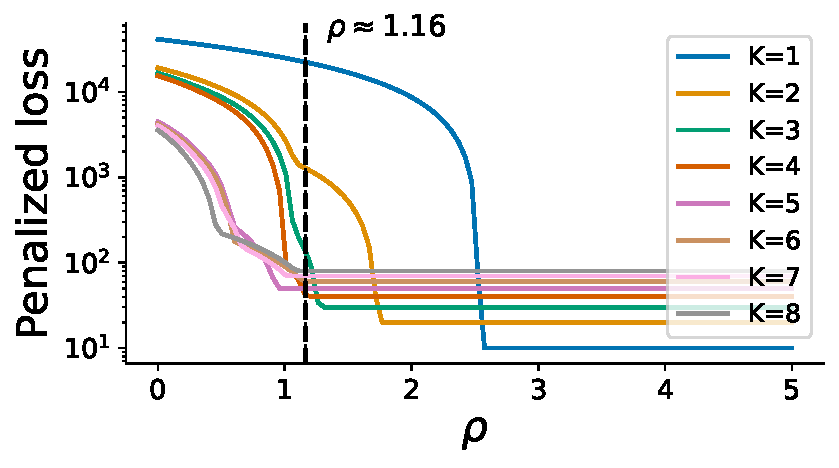
\includegraphics[width=.48\textwidth]{GvHD12-all-loss-plot-legend}}
	\caption{Calibration including $\numcomps=1,\ldots,8$ for test datasets 7--12 in flow cytometry experiments. }
	\label{fig:GvHD3}
\end{figure}



\section{Skew-normal Mixture Simulation Study}
\label{sec:simulation-gauss}

%We now provide further details about the motivating example in \cref{sec:motivation}, and illustrate
%that \methodname selects the correct number of components under a variety of conditions on the level of misspecification
%and the relative sizes of the mixture components.
%%To show the strength of structurally aware robust inference in the context of model misspecification, 
%We generate data $x_1, \ldots, x_n \in \mathbb{R}$ from skew-normal mixtures of the form $P_{o} = \sum_{k=1}^{\numcomps_{o}}\eta_{ok}\distSNorm(\mu_{ok}, \sigma_{ok},\gamma_{ok})$, where $\distSNorm(\cdot)$ denotes the skew-normal distribution and $\gamma_{ok}$ denotes the skewness parameter.
%The density of the skew-normal distribution $\distSNorm(\mu, \sigma,\gamma)$ is $f(x) = 2\phi(x;\mu,\sigma)\Phi(\gamma x;\mu,\sigma)$, where $\phi(x;\mu,\sigma)$ and $\Phi(x;\mu,\sigma)$ denote the probability density function and the cumulative distribution function of $\distNorm(\mu,\sigma)$ respectively.
%We model the data using  Gaussian mixture model $G_{\allparam} = \sum_{k=1}^{\numcomps}\eta_{k}\distNorm(\mu_{k}, \sigma_{k})$.
%The bigger $|\gamma_{ok}|$, the larger the deviation from the Gaussian distribution,
%hence introducing a higher degree of misspecification.

In \cref{sec:intro}, we consider the case of two clusters of equal size. 
We set $\eta_{o} = (0.5, 0.5)$, $\mu_{o} = (-3,3)$, and $\sigma_{o} = (1,1)$ for the two scenarios in \cref{fig:motivate-comparison}: $\gamma_o = (-10,-1)$ (denoted \texttt{different}) and $\gamma_o = (-10,-10)$ (denoted \texttt{same}).
We now compare \methodname to the coarsened posterior with data from
two-component mixtures of different cluster sizes. %, under which coarsened posterior fails. 
%The degree of misspecification is controlled by distributional parameters $\allparam_o = (\mu_{o}, \sigma_{o}, \gamma_{o})$. 
We set $\eta_{o} = (0.95, 0.05)$, $\mu_{o} = (-3,3)$, and $\sigma_{o} = (1,1)$ for the following three scenarios:
$\gamma_o = (-10,-1)$ (denoted \texttt{large-small}),  $\gamma_o = (-1,-10)$ (denoted \texttt{small-large}),
and  $\gamma_o = (-10,-10)$ (denoted \texttt{large-large}).

\begin{figure}[tp]
	\centering
	\subfloat{\label{fig:gauss-cpos-pdfs-1}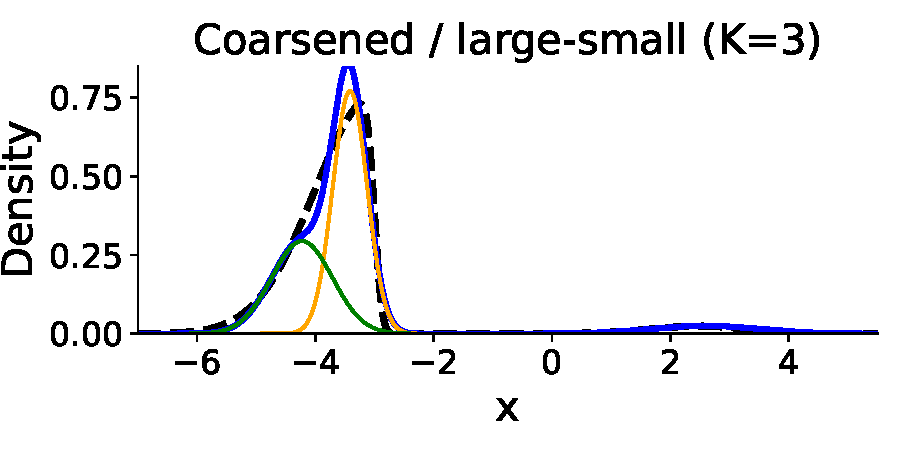
\includegraphics[width=.32\textwidth]{skewnorm-coarsen-pdfs-n=5000-close-False-rsize-big-small-rmis-big-small}}
	\subfloat{\label{fig:gauss-cpos-pdfs-2}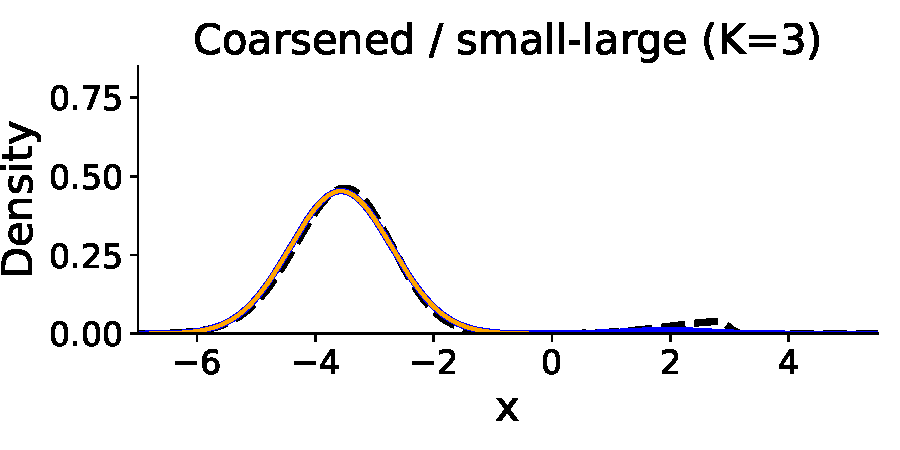
\includegraphics[width=.32\textwidth]{skewnorm-coarsen-pdfs-n=5000-close-False-rsize-big-small-rmis-small-big}}
	\subfloat{\label{fig:gauss-cpos-pdfs-3}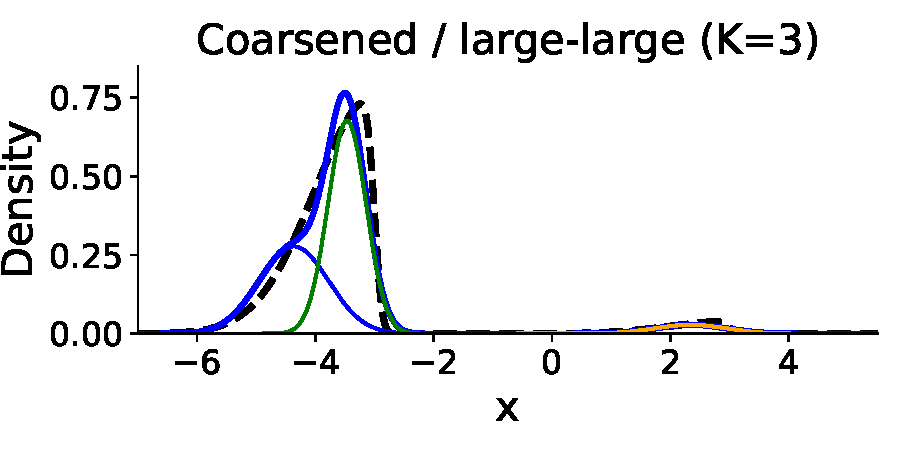
\includegraphics[width=.32\textwidth]{skewnorm-coarsen-pdfs-n=5000-close-False-rsize-big-small-rmis-equal}}
	\\
	\subfloat{\label{fig:gauss-stare-pdfs-1}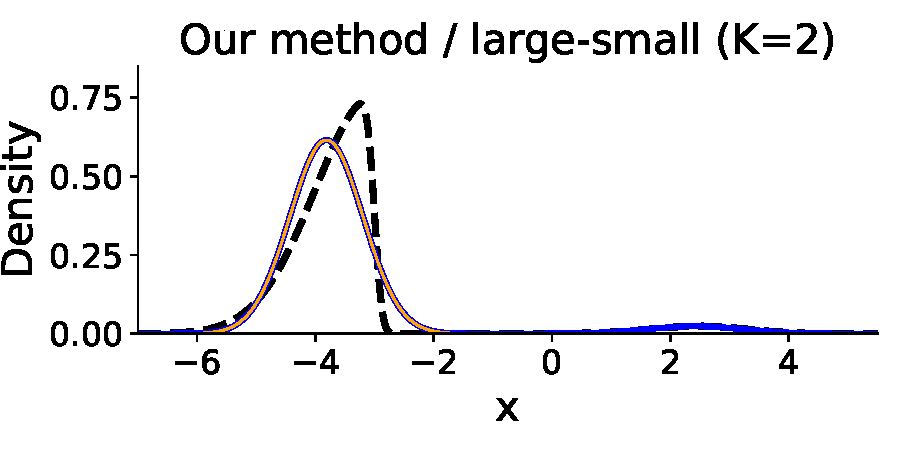
\includegraphics[width=.32\textwidth]{skewnorm-stare-pdfs-n=5000-close-False-rsize-big-small-rmis-big-small}}
	\subfloat{\label{fig:gauss-stare-pdfs-2}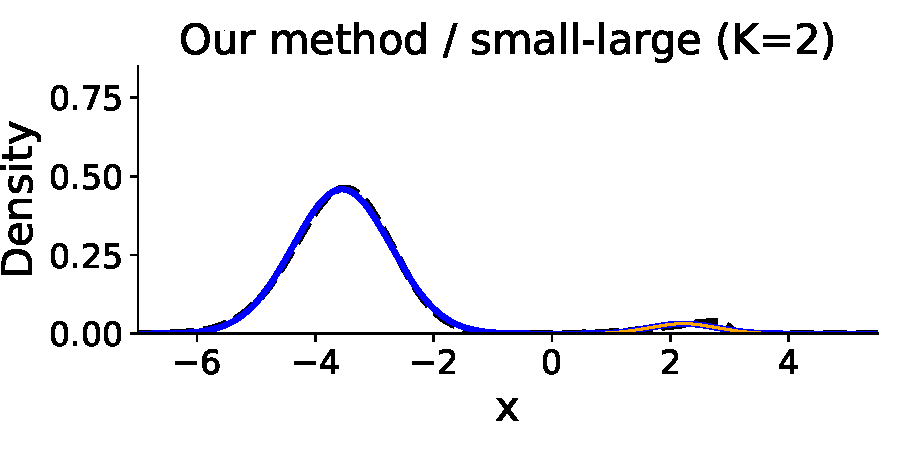
\includegraphics[width=.32\textwidth]{skewnorm-stare-pdfs-n=5000-close-False-rsize-big-small-rmis-small-big}}
	\subfloat{\label{fig:gauss-stare-pdfs-3}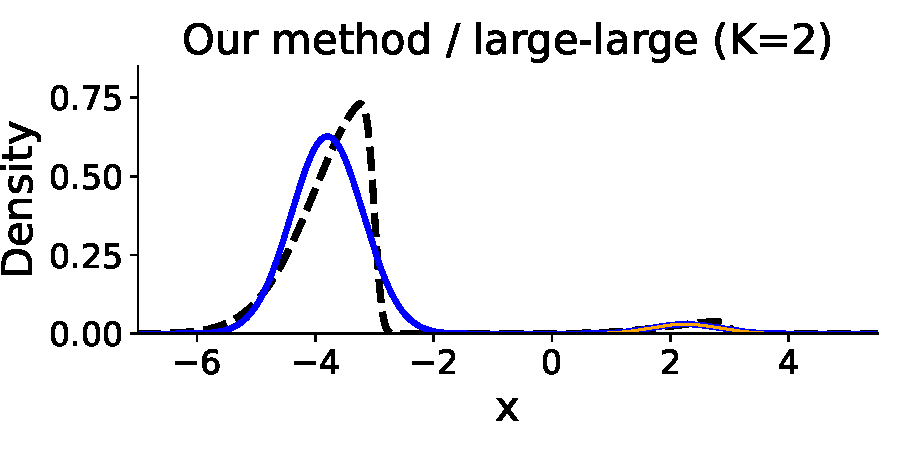
\includegraphics[width=.32\textwidth]{skewnorm-stare-pdfs-n=5000-close-False-rsize-big-small-rmis-equal}}
	\\
	\subfloat{\label{fig:gauss-stare-penloss-1}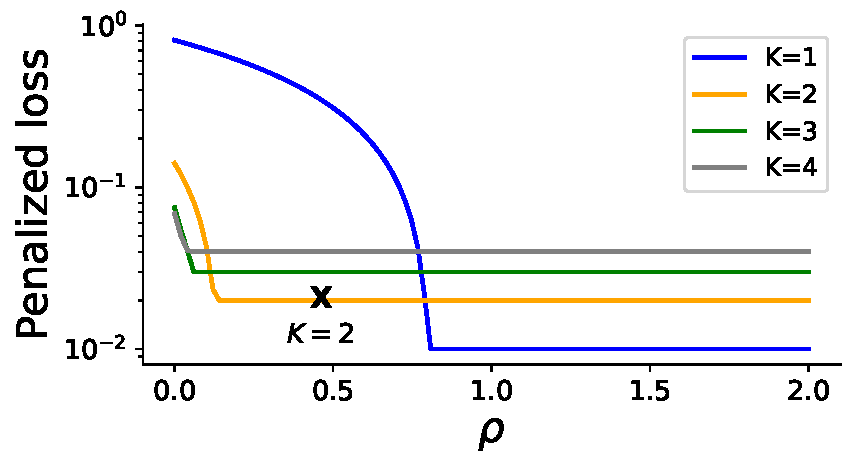
\includegraphics[width=.32\textwidth]{skewnorm-stare-loss-n=5000-close-False-rsize-big-small-rmis-big-small-legend}}
	\subfloat{\label{fig:gauss-stare-penloss-2}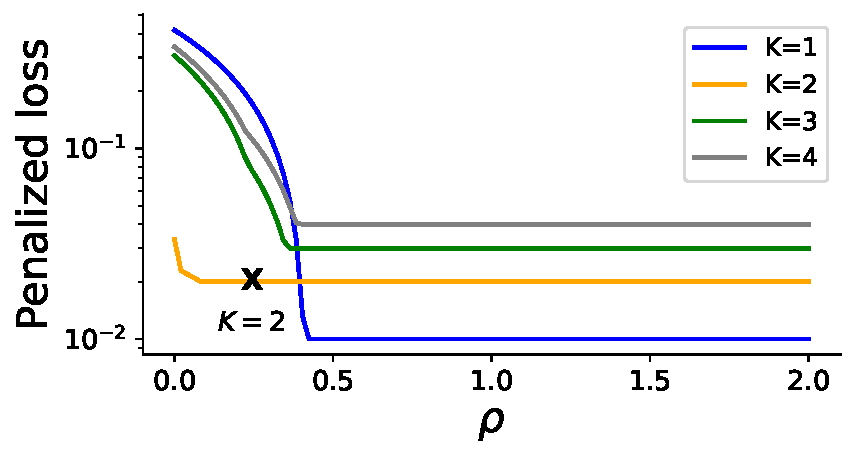
\includegraphics[width=.32\textwidth]{skewnorm-stare-loss-n=5000-close-False-rsize-big-small-rmis-small-big-legend}}
	\subfloat{\label{fig:gauss-stare-penloss-3}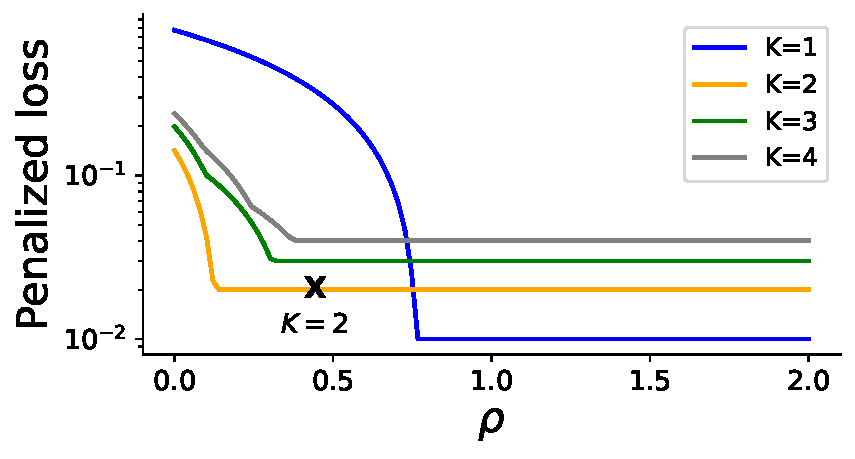
\includegraphics[width=.32\textwidth]{skewnorm-stare-loss-n=5000-close-False-rsize-big-small-rmis-equal-legend}}


	\caption{
		Comparison between the coarsened posterior and \methodname when using a Gaussian mixture model to fit data generated from a mixture of
		skew-normal distributions.
		\textbf{First row:} Densities of the model and components selected using the coarsened posterior (solid lines) and the density of the data distribution (dashed line). The title specifies the data-generating distribution and the number of components selected.
		In the middle plot of the first row, the minor cluster contains two components.
		\textbf{Second row:} Densities of the model and components selected using our structurally aware robust method.
		\textbf{Third row:} Penalized loss plots, where the cross mark indicates the first wide stable region and is labeled with the number of clusters \methodname selects.
		Line colors correspond to different $\numcomps$ values.}
	\label{fig:gauss-simulation}
\end{figure}

For the coarsened posterior, we calibrate the hyperparameter $\alpha$ following the procedure from \citet[Section 4]{Miller:2019}.
First, we use Markov chain Monte Carlo to approximate the coarsened posterior for $\alpha$ values ranging from $10$ to $10^5$.
Then, we select the coarsened posterior with the $\alpha$ value at the clear cusp that indicates a good fit and low complexity.
See the Supplementary Materials for further details and calibration plots.
%We then use the proposed $\alpha$ in the coarsening method to do inference for the same dataset. \PROBLEM{(1) For all experiments, we should include calibration plots for coarsened posterior and \methodname in the SM. It's OK if this results in some duplication.  }
%As shown in \cref{fig:gauss-simulation}, coarsened posterior fails in different ways. For Scenarios (\ref{gaussmix-s1}) and (\ref{gaussmix-s3}), the coarsened posterior tend to overfit the larger cluster. 
%For Scenario (\ref{gaussmix-s2}), the smaller cluster with more misspecification is underfit.
As shown for \texttt{large-small} and \texttt{large-large} in \cref{fig:gauss-simulation}, when the
larger cluster has large misspecification, the coarsened posterior introduces one additional cluster to explain the larger cluster.
For the \texttt{small-large} case, when the larger cluster exhibits a small degree of misspecification,
the coarsened posterior introduces one additional cluster to explain the smaller cluster.

%\NA{The reason behind these facts is that coarsened posterior posits robustness on the overall density estimation rather than from a component level. 
%It then tends to distribute the same degree of robustness tolerance to both clusters no matter how different their misspecification scaled by the cluster size are. 
%This finally leads to two potential misleading outcomes: overfit the cluster with larger scaled misspecification and underfit the cluster of smaller scaled misspecification.
%Therefore, when coarsened posterior learns about the tolerance level through hyperparameter $\alpha$, it picks up a choice that balances out the overall density estimation and the model complexity.
%The test data will then inherit the same spirit as in training dataset through the value of $\alpha$ and results in overfit or underfit outcomes.}\fTBD{JHH: I will revise this paragraph later}
%%Due to the criteria on achieving decent overall density estimation, when the size of clusters and level of misspecification differ significantly, coarsened posterior tends to either overlook smaller cluster or overfit larger clusters of more misspecification.

\methodname correctly calibrates the model mismatch cutoff $\rho$ using the penalized loss plots shown in \cref{fig:gauss-simulation},
as in all cases $\numcomps = 2$ corresponds to the first wide, stable region.
By the density plots in the middle column, we can see that \methodname 
is able to properly trade off a worse density estimate for better model selection.
%picks the correct number of components at a cost of negligible deviation from the true component distributions for all scenarios. 
%and discovers the true number of components in all 
%three cases. 
%%with the awareness of the structural causal structure and place the cutoff for components. 
%From  in , 
%we apply structurally aware robust selection rule to pick up the number of components $\numcomps$ corresponding to the first widest and stable region in penalized modified loss plot.
%In our case, the widest and stable region for the loss and value of $\rho$ appears when $\widehat{\numcomps}= 2$. This indicates a preference of choosing mixtures of $\widehat{\numcomps} = 2$ components.
%Our approach also enjoys improved computational efficiency compared to coarsened posterior (see discussion in \cref{sec:motivation}).
%\NA{The coarsened posterior is greatly slowed down by doing a grid search on the hyperparameter $\alpha$. Each value of $\alpha$ requires running a MCMC algorithm.
%However, structurally aware robust inference benefits from the piecewise linear relationship between the modified loss and robustness parameter $\rho$, which facilitates the calibration of parameter $\rho$ value without doing a grid search.}\fTBD{This part might be redundant; revisit once earlier sections are locked in}
%This is verified in the runtime comparison that running one scenario using our structurally aware robust model selection method (code in Python) takes about 1 minute
%while using the coarsened posterior (code in Julia) takes 140 minutes, despite Julia generally being much faster than Python in scientific computing applications \citep{Perkel:2019}.

%Therefore, we expect the structurally aware robust inference leads to a better accommodation to clusters of different levels of misspecification.




\section{Reverse sampling}

\subsection{Poisson NMF}

Recall the standard Poisson NMF model:
\[
	{y}^{(K)}_{nk}& \distas \distPoiss\lrp{{\phi}^{(K)}_{k}z^{(K)}_{nk}} \quad&&\text{for}\ n=1,\dots,N,k=1,\dots,K\\
	{x}_{n}&=\sum^{K}_{k=1}{y}^{(K)}_{nk}\quad&&\text{for}\ n=1,\dots,N,
\]
Applying Bayes' rule, we can sample ${\veps}_{nk}\mid{x}_{n}$ for any given $n,k$ using the following procedure, with
each dimension $d$ sampled independently:
\[
	{y}^{(K)}_{n,1:K,[d]}\mid{x}_{n,[d]}&\sim \distMulti \lrp{{x}_{n,[d]};\widehat{p}_{n,1:K,d}}, \\
	{\veps}_{n,k,[d]}\mid{y}^{(K)}_{n,k,[d]}&\sim\Unif\left(\mathcal{F}_{\distPoiss}\lrp{y^{(K)}_{n,k,[d]}-1;p_{n,k,d}},\right.
	% &\quad\quad\quad
	\left.\mathcal{F}_{\distPoiss}\lrp{{y}^{(K)}_{n,k,[d]};p_{n,k,d}}\right),
	\label{eq:Pois_eps_sampling}
\]
where
\[
	p_{n,k,d} &= {\phi}^{(K)}_{k,[d]}z^{(K)}_{nk}, &
	\widehat{p}_{n,k,d} &= \frac{p_{n,k,d}}{\sum^{K}_{k'=1}p_{n,k',d}},
\]
and $\mathcal{F}_{\distPoiss}(\blank;\lambda)$ is the cdf of $\distPoiss(\lambda)$.

\subsection{Normal Factor Analysis Model}

Recall the usual Gaussian factor analysis model: 
\[
	\begin{aligned}
		{\Sigma}^{(K)}_{k} & =\lrb{\sigma^{2}_{k, 1},\dots,\sigma^{2}_{k, D}}\transpose&& \text{for}\ k=1,\dots,K, \\
		{y}^{(K)}_{nk}          & \mop{\sim}^{\mathrm{e.w}} \distNorm\lrp{{\phi}^{(K)}_{k}z^{(K)}_{nk},{\Sigma}^{(K)}_{k}}
		\qquad\quad&& \text{for}\ n=1,\dots,N,k=1,\dots,K,                        \\
		{x}_{n}           &=\sum^{K}_{k=1}{y}_{nk}&& \text{for}\ n=1,\dots,N.
	\end{aligned}
\]
Again, applying Bayes' rule, we can sample ${\veps}_{nk}\mid{x}_{n}$ for any given $n,k$ using the following formulation, 
with each dimension $d$ sampled independently:
\[
	&{y}^{(K)}_{n,k,[d]}\mid{x}_{n,[d]},y^{(K)}_{n,1:k-1,[d]},\sigma_{1:K,d}\sim
	\left\{\begin{array}{lr}
		\distNorm(\widetilde{\mu}_{n,d,k},\widetilde{\sigma}^{2}_{k,d}) & \text{if}\ k\neq K, \\
		\delta\lrp{\overline{x}_{n,k,d}}                              & \text{if}\ k=K,
	\end{array}\right. \\
  &{\veps}_{n,k,[d]} = \mathcal{F}_{\distNorm}
	\lrp{{y}^{(K)}_{n,k,[d]};\mu_{n,k,d},\sigma^{2}_{k,d}},
\]
where
\[
	&\overline{x}_{n,k,d}={x}_{n,[d]} - \sum^{k-1}_{k'=1} {y}^{(K)}_{n,k',[d]},
	&\mu_{n,k,d}={\phi}^{(K)}_{k,[d]}z^{(K)}_{nk},\\
	&\overline{\mu}_{n,k,d}=\sum^{K}_{k'=k+1}\mu_{n,k',d}, %{W}^{(K)}_{[d,k']}{h}^{(K)}_{n,[k']},
	&\overline{\sigma}^{2}_{k,d}=\sum^{K}_{k'=k+1}\sigma^{2}_{k',d},\\
	&\widetilde{\mu}_{n,k,d}=\frac{\sigma^{-2}_{k,d}\mu_{n,k,d}-
		\overline{\sigma}_{k,d}^{-2}(\overline{\mu}_{n,k,d}-\overline{x}_{n,k,d})}
	{\sigma^{-2}_{k,d}+\overline{\sigma}^{-2}_{k,d}},
	&\widetilde{\sigma}^{2}_{k,d}=\frac{\sigma^{2}_{k,d}\overline{\sigma}^{2}_{k,d}}
	{\sigma^{2}_{k,d}+\overline{\sigma}^{2}_{k,d}},
\]
and $\mathcal{F}_{\distNorm}(\blank;\mu,\sigma^{2})$ is the cdf of $\distNorm(\mu,\sigma^{2})$. 
%Note that ${y}^{(K)}_{n,k,[d]}$ is sampled sequentially with respect to $k$ and is conditioned on all previously sampled ${y}^{(K)}_{n,k',[d]}$ where $1\leq k'<k$.

\begin{figure}[]
  \centering
  \subfloat[Well specified]{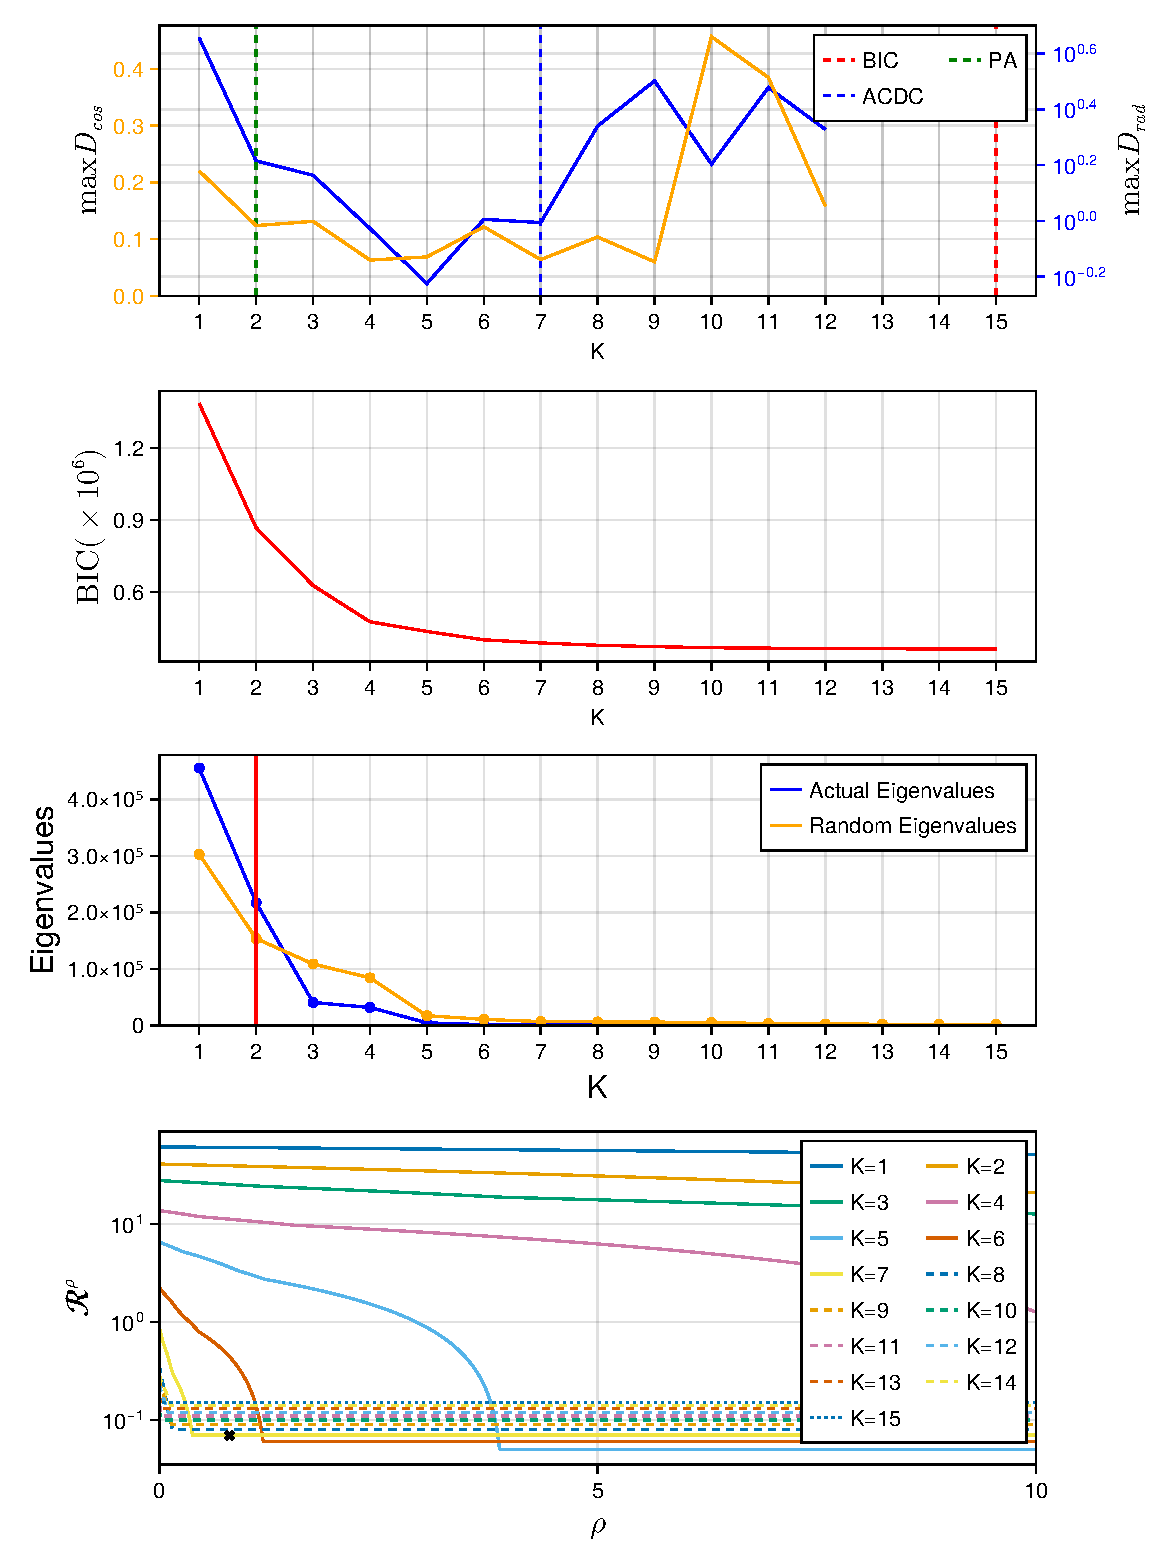
\includegraphics[width=\textwidth]{figures/composite-multdiv-600-breast-custom-seed-1.pdf}}\\
  \caption{Estimation quality for various scheme of data generation. See \cref{fig:mutsig_result} caption for explanation.}
  \label{fig:mutsig_result_appendix_1}
\end{figure}

\begin{figure}[]\ContinuedFloat
  \centering
  \subfloat[Contaminated]{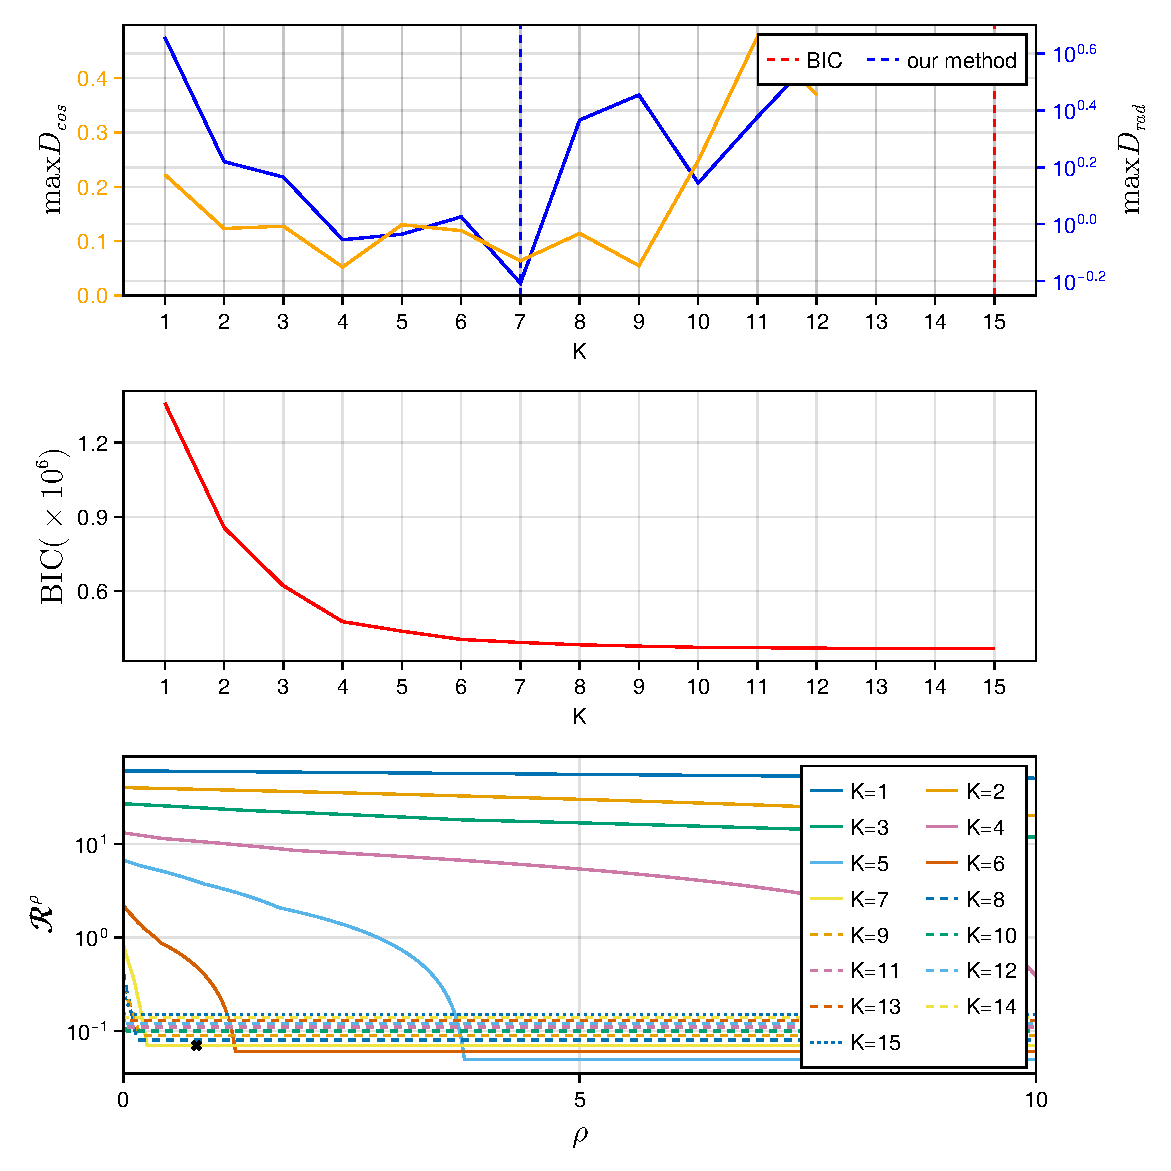
\includegraphics[width=\textwidth]{figures/composite-multdiv-600-breast-custom-seed-1-contamination-2.pdf}}\\
  \caption{Estimation quality for various scheme of data generation. See \cref{fig:mutsig_result} caption for explanation.}
  \label{fig:mutsig_result_appendix_2}
\end{figure}

\begin{figure}[]\ContinuedFloat
  \centering
  \subfloat[Overdispersed]{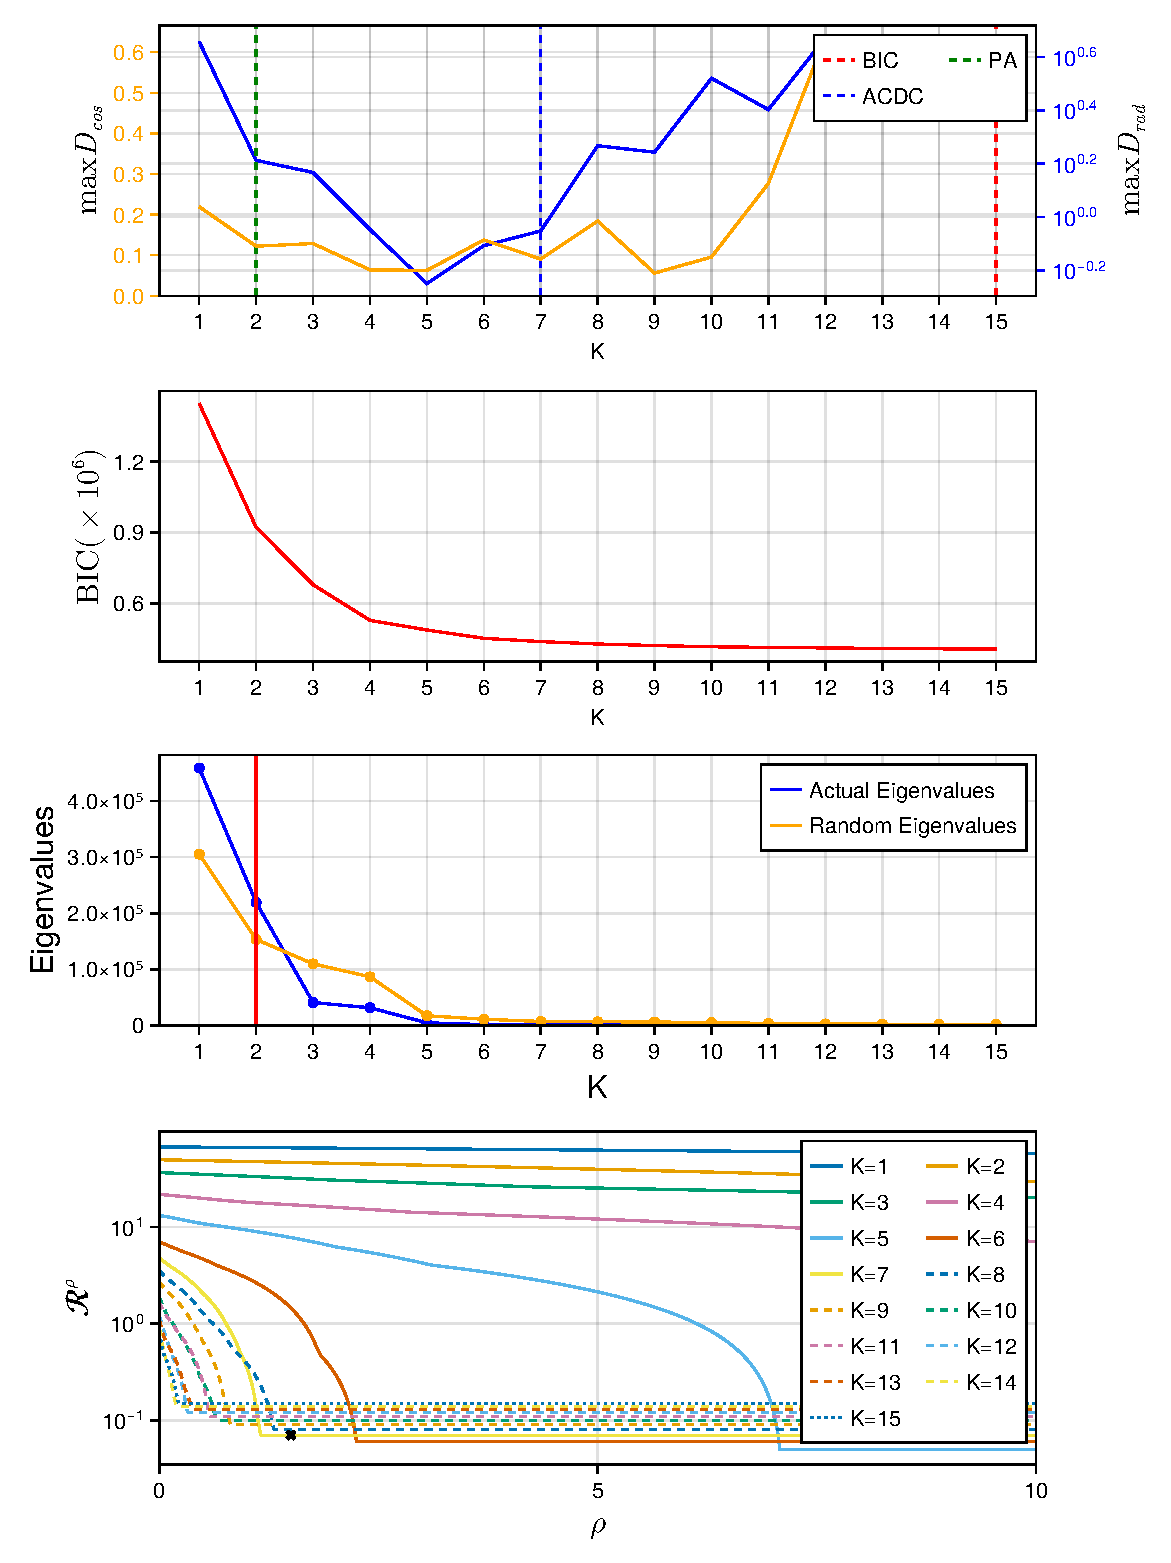
\includegraphics[width=\textwidth]{figures/composite-multdiv-600-breast-custom-seed-1-overdispersed-2.0.pdf}}
  \caption{Estimation quality for various scheme of data generation. See \cref{fig:mutsig_result} caption for explanation.}
  \label{fig:mutsig_result_appendix_3}
\end{figure}

\begin{figure}[]\ContinuedFloat
  \centering
  \subfloat[Perturbed]{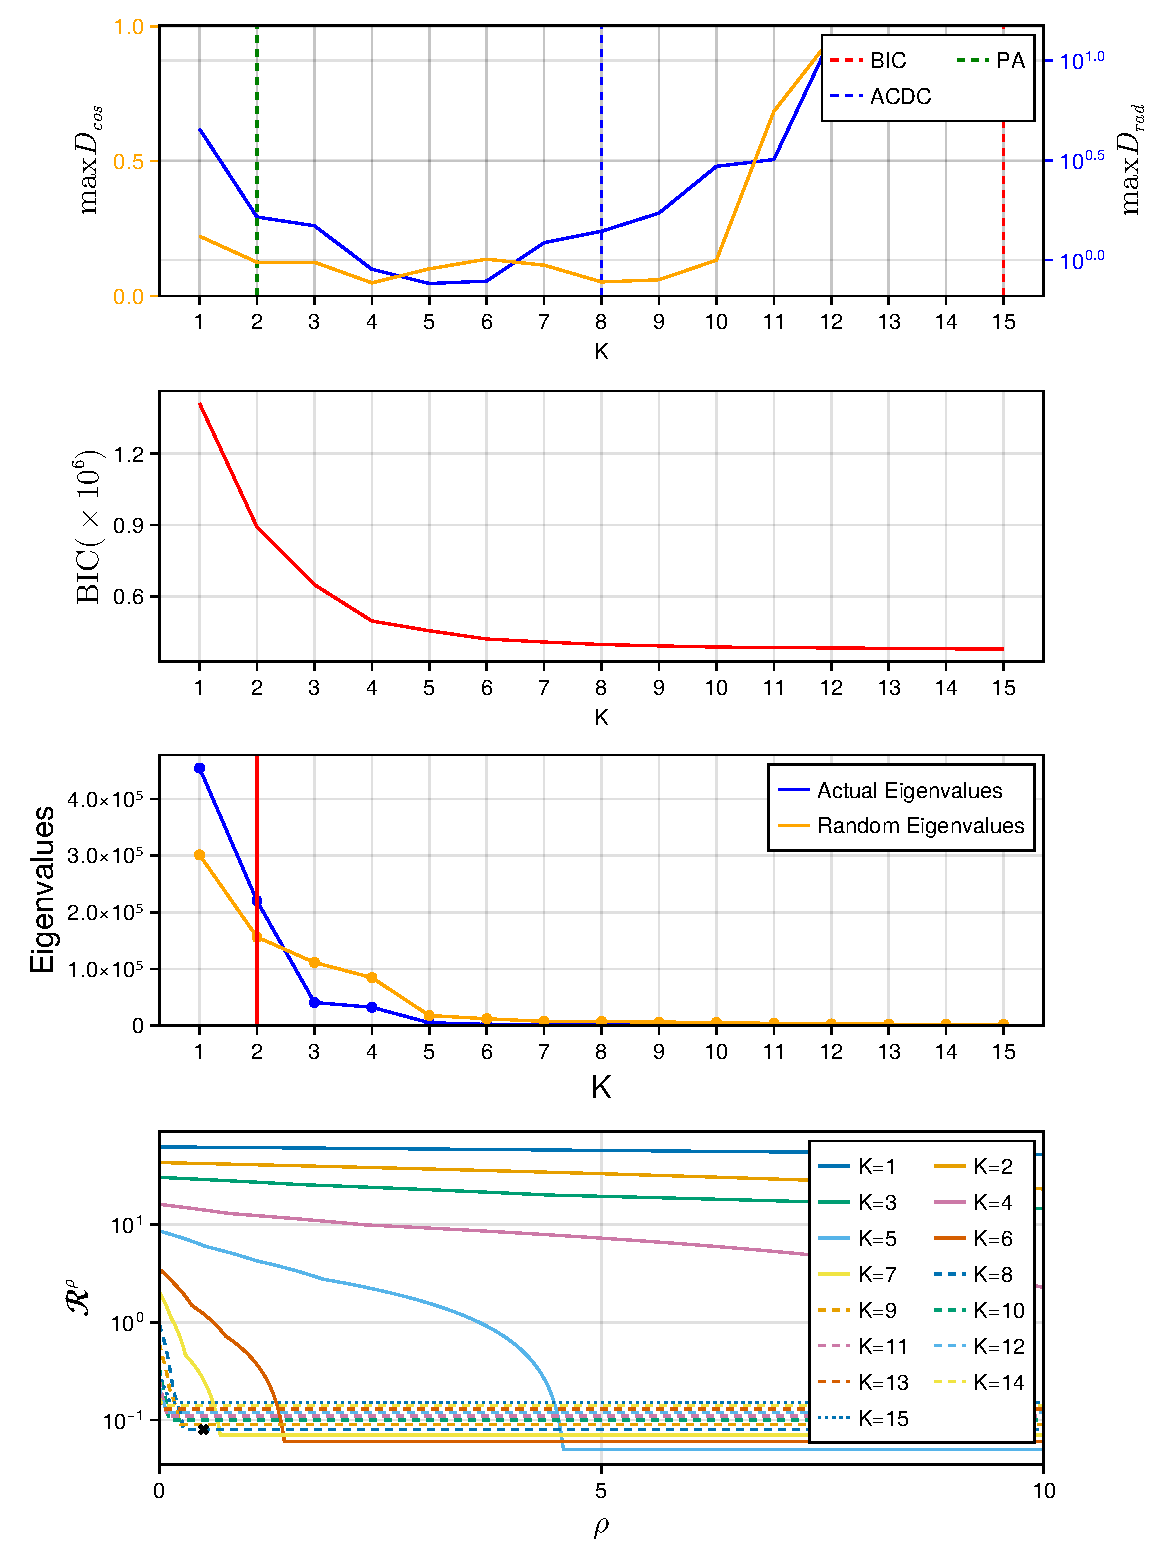
\includegraphics[width=\textwidth]{figures/composite-multdiv-600-breast-custom-seed-1-perturbed-0.0025.pdf}}
  \caption{Estimation quality for various scheme of data generation. See \cref{fig:mutsig_result} caption for explanation.}
  \label{fig:mutsig_result_appendix_4}
\end{figure}

\begin{figure}[h!]
	\centering
  \subfloat[Unlabeled (left) and labeled (right) versions of the urban dataset]{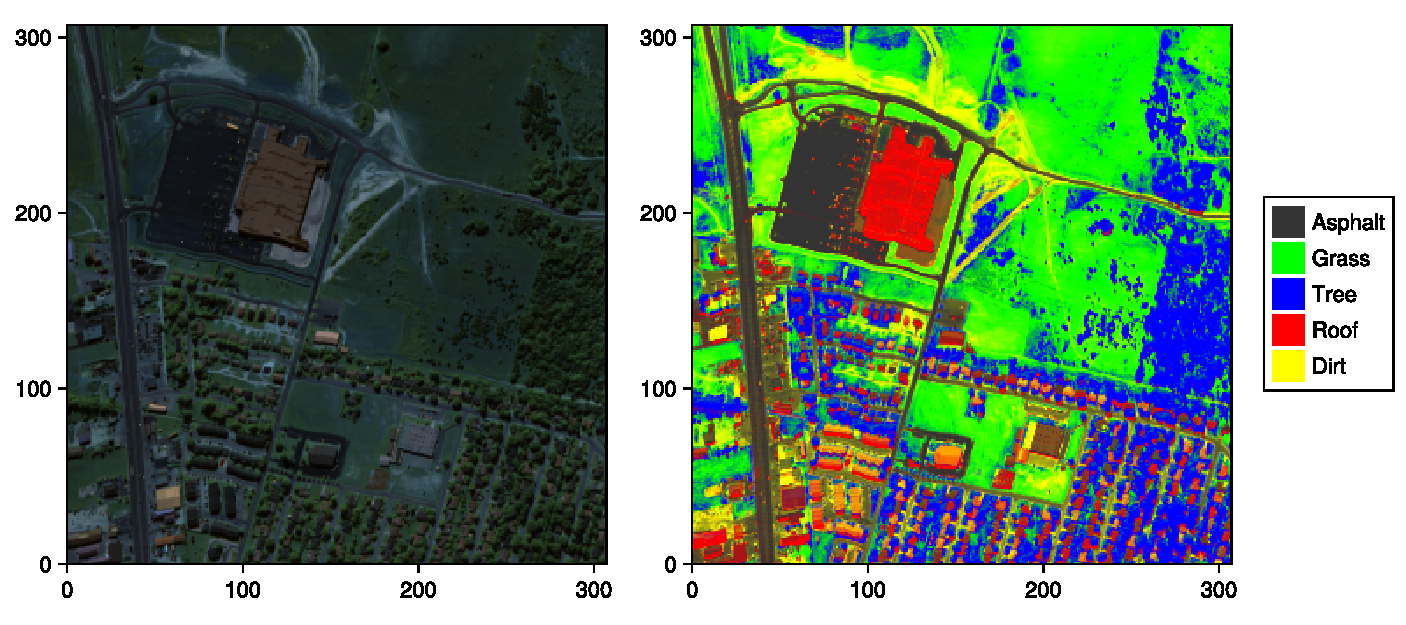
\includegraphics[width=0.9\textwidth]{./figures/urban_gt_5endmembers.pdf}}\\
	\subfloat[$K=3$]{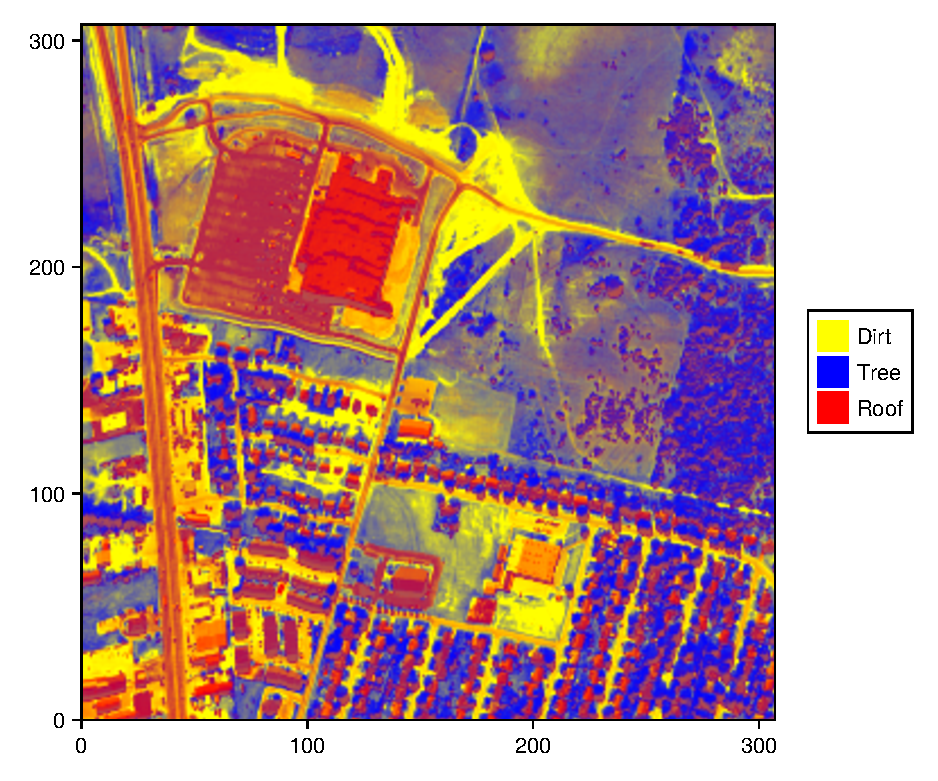
\includegraphics[width=0.45\textwidth]{figures/urban_K=3.pdf}}
	\subfloat[$K=4$]{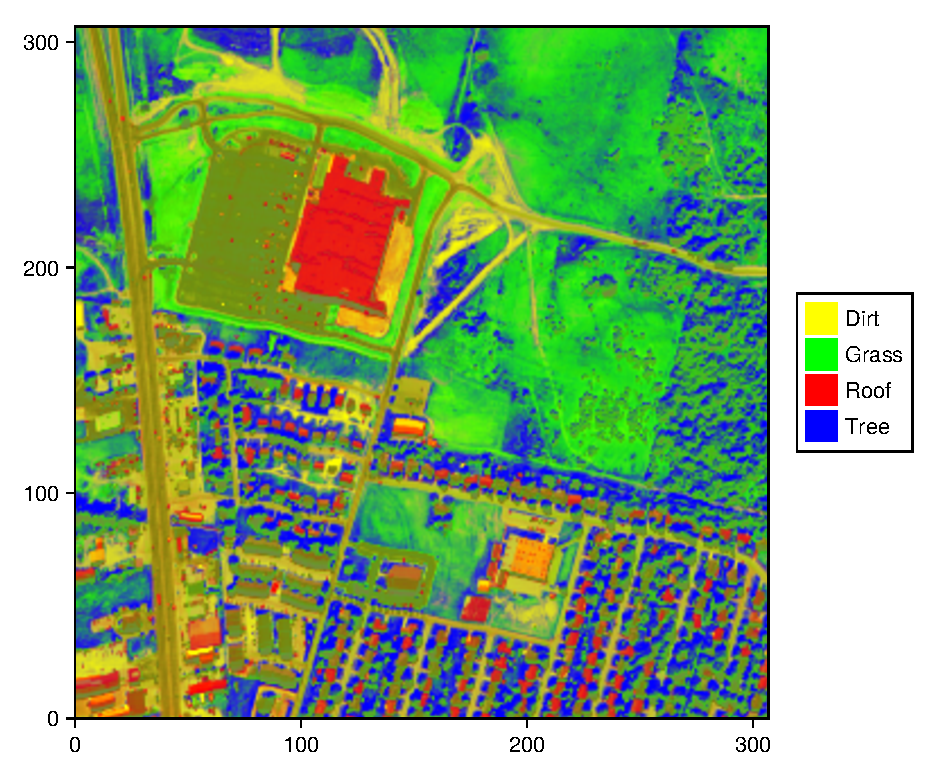
\includegraphics[width=0.45\textwidth]{figures/urban_K=4.pdf}}\\
	\subfloat[$K=5$]{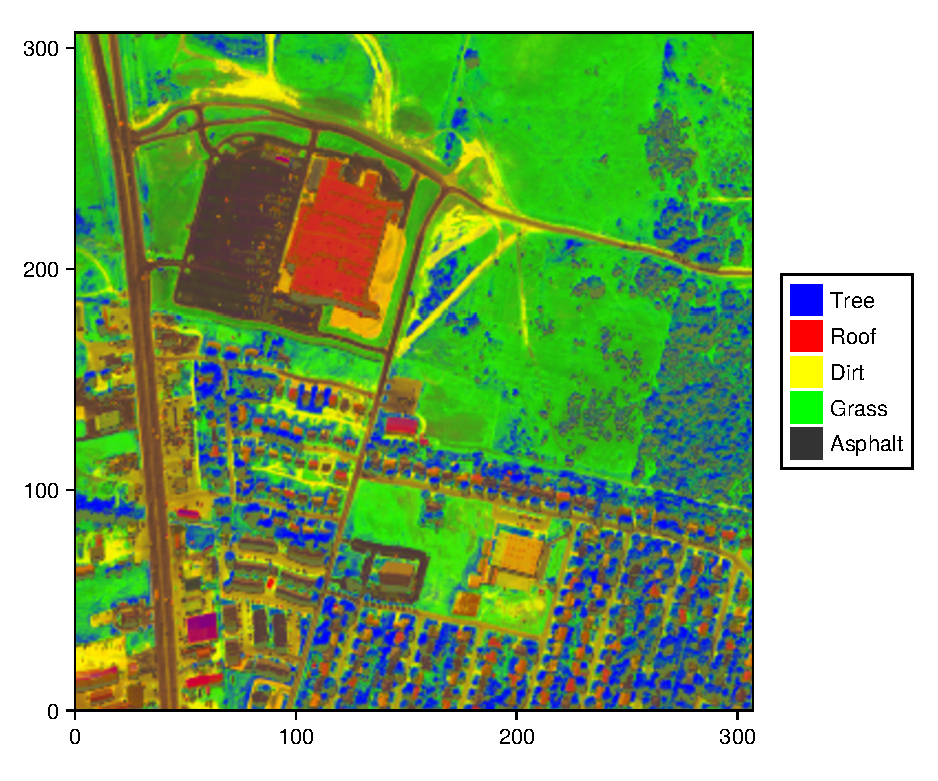
\includegraphics[width=0.45\textwidth]{figures/urban_K=5.pdf}}
	\subfloat[$K=6$]{\includegraphics[width=0.45\textwidth]{figures/urban_K=6.pdf}}
  \caption{Visualization of the hyperspectral urban datasets.
  \textbf{(a)} Data and ground truth labels.
  \textbf{(b, c, d, e)} Inferred end-member abundance maps for $K=3,4,5,6$.}
	\label{fig:hyprunmix_gt}
\end{figure}

\section{Additional Case Study Experimental Details and Results}
\label{sec:case-study-details}

\begin{figure}[tp]
	\centering
	% \subfloat{\includegraphics[width=0.54\textwidth]{comp_ari_hist.pdf}}
	% \subfloat{\includegraphics[width=0.43\textwidth]{comp_autosarm.pdf}}

    % \subfloat{\includegraphics[width=0.54\textwidth]{comp_ari_hist_80uniform.pdf}}
    \subfloat{\includegraphics[width=0.54\textwidth]{comp_ari_hist_80uniform_0cent.pdf}}
	% \subfloat{\includegraphics[width=0.43\textwidth]{comp_autosarm_80uniform.pdf}}
    \subfloat{\includegraphics[width=0.36\textwidth]{automanSARM_comp_uniform.pdf}}


	\caption{Comparison between manual and automated selection of $\rho$ for the \textsf{uniform} scRNA-seq datasets. 
        \textbf{Left:} Pairwise difference in ARI. 
		\textbf{Middle:} Pairwise difference in AMI.
		\textbf{Right:}
		% True number of cell types vs. estimated number of cell types in concatenated tissue datasets (with x-axis jitter)}.
        Manually vs. automatically estimated number of cell types in uniform datasets (with x-axis jitter).} 
	\label{fig:auto_comp_unif}
\end{figure}

\subsection{Data Overview and Processing}
\label{sec:rna-data}
%(scRNA-seq)

Tabula Muris \citep{mice}
is a comprehensive collection of single-cell transcriptome data.
The gene count tables are derived from SMART-Seq2 RNA-seq libraries and consist
of 53,760 cells from 20 different organs and tissues of 8 mice. 
%This dataset includes 53,760 cells collected from 20 tissues of 8 mice.
%
% For gene expression matrix $\mathrm{X}_{D \times N}$
% for $D$ genes and $N$ single cell observations, we assume for cell $j\in \{ 1,\ldots,N\}$, %the vector of gene expression, 
% the log transformed counts $x_{\cdot j}$, given cell type $k$,
% follows a Gaussian distribution %$x_i \sim 
% $N(\mu_k,\Sigma_k)$
% where $\mu_k$ and $\Sigma_k$ are the mean and covariance of the $k$-th mixture component.
% Then, for each cell $j$, the data can be written in the form of a
% Gaussian mixture distribution
% $x_{\cdot j}\sim p(x) = \sum_{k=1}^{K_o} \eta_k \cdot N(x|\mu_k,\Sigma_k)$ where $\eta_k$ is the probability that an observation belongs to cluster $k$ and $\sum_{k=1}^{K_o} \eta_k = 1 $.
% To ensure consistent evaluation of the clustering performance of \methodname over a range of possible true number of cell types, 
We subsampled datasets from the Tabula Muris data while controlling for the number of cell types and the number of cell observations in each cell type.
We constructed 80 \textsf{uniform} datasets using 8 experimental settings and 10 replications each, as
described in \cref{tab:subsampled-datasets}.
%
\begin{table}[tp]
	\centering
	%\def~{\hphantom{0}}
	%\tbl
	\caption{Summary of uniform cluster data:
		A total number of $E=8$ experiment settings, each with $10$ replications, resulting in experiments with 8 different numbers of cell types: $T = 2\times[E]  =  \{2,4,…,16\}$, where each cell type has $ N_T = 500$ cell observations. Each experiment has total cell observations $t\times N_t=500\times t,\ \forall \, t\in T$.}{
		\begin{tabular}{cccc}
			\hline
			\textbf{Experiment Settings (E)} & \textbf{Cell Types (T)}   & \textbf{Cell Observations}           & \textbf{Replications} \\ \hline
			8                                & $\{2, 4, 6, \ldots, 16\}$ & $500 \times T$ (from 1,000 to 8,000) & 10 per setting        \\ \hline
		\end{tabular}}
	\label{tab:subsampled-datasets}
\end{table}
%
%Recognizing that real-world scenarios often involve varying cell type proportions, 
We also generated 15 \textsf{nonuniform} datasets with variably sized clusters using three sets of concatenated tissue data (\cref{tab:datasets}).
For each of the three sets, we downsampled them to create 4 additional datasets, resulting in 15 datasets total.
%subsample technique
\begin{table}[tp]
	\centering
	%\def~{\hphantom{0}}
	%\tbl
	\caption{Summary of non-uniform cluster data: The number of cells of each type in each dataset were downsampled with proportions 1 (no downsampling), 0.6, 0.36, 0.21, and 0.13, resulting in a total of 15 samples. }{
		\begin{tabular}{cccc}
			\hline
			%\textbf{Dataset} & 
			\textbf{Cell Observations} & \textbf{Cell Types} & \textbf{Tissue}                               \\ \hline
			%1 & 
			8,082                      & 13                  & large intestine, trachea, bladder, and tongue \\
			%2 & 
			8,235                      & 15                  & brain myeloid, kidney, spleen, and pancreas   \\
			%3 & 
			9,811                      & 16                  & thymus, fat, mammary gland, and limb muscle   \\ \hline
		\end{tabular}}
	\label{tab:datasets}
\end{table}
%
%data processing 

All datasets were processed according to the following procedure using the Seurat R package before being used for clustering.
Cells with low gene counts ($<200$) and genes expressed in very few cells ($<2$) are excluded.
The gene expression counts are normalized and log-transformed by each cell.
After log transformation, the counts are scaled so that each gene has a mean expression of 0 and a variance of 1 across all cells.
Finally, PCA is performed on a subset of highly variable genes that exhibit significant variation across cells, and the projected data dimension is determined by the Jackstraw method \citep{Chung_jackstraw}.

We evaluate cell clustering performance by examining both the accuracy of cluster assignments and the precision in estimating the number of cell types.
To test whether \methodname effectively prevents overestimation, we examine the deviation of the estimate from the true number of cell types $K_o$. The agreement between the ground truth labels and the estimated labels is quantified using the Adjusted Rand Index (ARI) and Adjusted Mutual Information (AMI).
For both ARI and AMI, a value of 1 indicates a perfect agreement between the compared clusters, and 0 indicates random clustering.
%
\begin{table}[tp]
	\centering
	%\def~{\hphantom{0}}
	%\tbl
	\caption{Sinkhorn parameter settings}{
		\begin{tabular}{cccc}
			\hline
			\textbf{Data Dimension} & \textbf{$\gamma, c$} & \textbf{$\varepsilon$} & \textbf{$\rho_1, \rho_2$} \\ \hline
			$\leq 20$               & Uniform              & 1                   & 20                        \\
			21--30                  & Uniform              & 2                   & 10                        \\
			31--60                  & Uniform              & 2                   & 5                         \\ \hline
		\end{tabular}}
	\label{tab:parameter-settings}
\end{table}


\subsection{Sinkhorn Distance}
\label{sec:sinkhorn}
%One benefit of our approach is the ability to use a wide range of discrepancy measures. 
%This flexibility allows the user to select a discrepancy that best captures the underlying structure of the data.
%%and hence makes the framework suitable for diverse clustering scenarios. 
%While the Kullback–Leibler divergence provides good default option, 
%the Wasserstein distance can better capture the underlying metric structure of the data.
% 
While the Wasserstein distance has appealing properties, it can be challenging to obtain an accurate estimate from finite samples
because it is sensitive to small changes in empirical distributions and suffers from slow convergence rates in high dimensions. 
The Sinkhorn distance, however, provides a regularized alternative that approximates the Wasserstein distance with faster sample convergence \citep{fast_sh}.
So, in practice, we can use the Sinkhorn distance to approximate the Wasserstein distance, 
which is the approach we take in \cref{sec:case-study}. 
Specifically, we use the unbalanced Sinkhorn distance \citep{unbsinkhorn}, which solves an unbalanced optimal transport (OT) problem
 in the discrete setting.
 Given samples $x_{1},\dots,x_{N}$ and $y_{1},\dots,y_{L}$, we can construction the 
cost matrix $M \in \reals^{N \times L}$ for a metric $m$ defined by $M_{n\ell} = m(x_{n}, y_{\ell})$. 
% Let $U(r, c)$ denote the set of transport plans that preserve the marginals $r$ and $c$: 
% \[
% U(r, c) = \left\{ P \in \mathbb{R}_+^{D \times D} \mid P {1}_D = r, P^T {1}_D = c \right\},
% \]
Let $U$ denote the set of transport plans 
\[
U = \left\{ A \in \mathbb{R}_+^{D \times D} \mid {1}_D^T A {1}_D = 1 \right\},
\]
where $1_{D}$ denotes the $D$-dimension vector with all components equal to 1. 
Given nonnegative regularization constants $\veps$ and $\varrho$, for $r \in \Delta_{N}$ and $c \in \Delta_{L}$,
the unbalanced Sinkhorn distance is defined as
% \[
% 	d_{M,\varepsilon, \rho}(r, c) = \min_{A \in U(r, c)}  \langle A, M \rangle + \varepsilon\,\kl{A}{rc^T}
% 	+ \rho_1\,\kl{A 1}{r}
% 	+ \rho_2\,\kl{A^T 1}{c}, 
% \]
\[
	d_{M,\varepsilon, \varrho}(r, c) = \min_{A\in U
    % (r, c)
    } \mathrm{tr}(A^{\top}M) + \varepsilon\,\kl{A}{rc^T}
	+ \varrho\,\kl{A 1}{r}
	+ \varrho\,\kl{A^T 1}{c}. 
\]
% where  $A$ is the transport plan, and  $r$ and $c$ are vectors representing discrete probability distributions.
% and $U(r, c)$ is the set that contains all transport plans $A$ that preserve the marginals $r$ and $c$ such that
% $U(r, c) = \left\{ A \in \mathbb{R}_+^{d \times d} \mid A {1}_d = r, P^T {1}_d = c \right\}$.
A larger value of $\varepsilon$ encourages a smoother, more numerically stable transport plan by penalizing the divergence between 
the plan $A$ and the independence (maximum entropy) transport plan $rc^T$. 
%which are numerically stable and less sensitive to small changes in $M$.
Smaller marginal penalty $\varrho$ introduces robustness to the marginal constraints of the transport plan.
The so-called balanced OT is retrieved in the limit of $\rho \to \infty$.
Additionally taking $\varepsilon\to0$ recovers the unregularized OT, which is equal to the
empirical 1-Wasserstein distance. 
%As $\varepsilon \to 0$ and $\rho \to + \infty$, the Unbalanced Sinkhorn converges to Wasserstein-1 ($d_W$) 

\subsection{Description of Existing Tools} \label{sec:existing-tools}

The Seurat R package \citep{seurat} uses a clustering algorithm based on shared nearest neighbor (SNN) modularity optimization.
%
Seurat first constructs a k-nearest neighbor (KNN) graph based on the Euclidean distance in the PCA space. A SNN graph is then constructed where edges are determined by the shared nearest neighbors among cells in the KNN graph.
% 
The weights are assigned to the edges so that the edges connecting cells sharing close nearest neighbors are weighted higher compared to those joining cells sharing distant nearest neighbors.
Finally, the SNN graph is partitioned into clusters using the Louvain algorithm, which optimizes the modularity of the clustering solution.

The SC3 \citep[Single-Cell Consensus Clustering;][]{sc3} R package employs a robust consensus clustering approach that integrates PCA, K-means, and hierarchical clustering.
Distance matrices are computed using Euclidean, Pearson, and Spearman metrics and transformed using PCA. The transformed distance matrices are used for K-means clustering, and multiple clustering solutions are generated based on different numbers of eigenvectors of the matrices. A cell-to-cell binary similarity matrix is constructed for each clustering result with each entry indicating whether two cells belong to the same cluster. These similarity matrices are averaged to form a consensus matrix that is then clustered using agglomerative hierarchical clustering where the clusters are identified at a user-specified level of hierarchy. For our experiments, we use the cluster number estimation function provided by the package to determine $K$.


\subsection{Results for Nonuniform Datasets}
\label{sec:non-unif-data}
% In this section, we present the result for the \textsf{nonuniform} datasets described in \cref{tab:parameter-settings}.
% To compare the clustering performance of \methodname with automatically and manually selected $K$, we analyzed pairwise differences in ARI and AMI across clustering results of the non-uniform cluster data and evaluate their difference in estimating the number of cell types. 
\begin{figure}[tp]
	\centering
	% \subfloat{\includegraphics[width=0.54\textwidth]{comp_ari_hist.pdf}}
    \subfloat{\includegraphics[width=0.54\textwidth]{comp_ari_hist_prop_0cent.pdf}}
	% \subfloat{\includegraphics[width=0.43\textwidth]{comp_autosarm.pdf}}
    \subfloat{\includegraphics[width=0.36\textwidth]{automanSARM_comp_prop.pdf}}

    % \subfloat{\includegraphics[width=0.54\textwidth]{comp_ari_hist_80uniform.pdf}}
	% \subfloat{\includegraphics[width=0.43\textwidth]{comp_autosarm_80uniform.pdf}}
    % \subfloat{\includegraphics[width=0.36\textwidth]{automanSARM_comp_uniform.pdf}}


	\caption{Comparison between manual and automated selection of $\rho$ for scRNA-seq clustering. 
        \textbf{Left:} Pairwise difference in ARI. 
		\textbf{Middle:} Pairwise difference in AMI.
		\textbf{Right:}
		% True number of cell types vs. estimated number of cell types in concatenated tissue datasets (with x-axis jitter)}.
        Manually vs. automatically estimated number of cell types in concatenated tissue datasets (with x-axis jitter).} 
	\label{fig:auto_comp}
\end{figure}
As shown in \cref{fig:auto_comp}, for the \textsf{nonuniform} data, 
the manually selected $K$ achieves slightly better ARI values (differences ranging from $-0.033$ to $0.045$), 
while automated $K$ selection results in higher AMI values (differences ranging from $0$ to $0.110$). 
To assess whether the differences are significant, we conduct paired t-tests on the AMI and ARI scores. For AMI, the mean
difference between the two methods is $0.0135$  (95\% CI: $[-0.0047, 0.0317])$. 
For ARI, the mean difference is $0.0011$ (95\% CI: $[-0.0071, 0.0094])$.
Hence, there appears to be no practically significant difference between the automated and manual approaches in terms of the two evaluation metrics.
On the other hand, the automated $K$ selection procedures occasionally significantly overestimates the number of cell types, so some care 
is required when using it. 
% 
\begin{figure}[tp]
	\centering
	\subfloat{\includegraphics[height=.25\textwidth,trim=0in 0in 1.35in 0in,clip]{tool_comp_prop_estk.pdf}}
	\subfloat{\includegraphics[height=.25\textwidth,trim=0in 0in 1.35in 0in,clip]{tool_comp_prop_ari.pdf}}
    \subfloat{\includegraphics[height=.25\textwidth]{tool_comp_prop_ami.pdf}}
	\caption{Comparison between \methodname and existing tools across concatenated tissue datasets
    \textbf{Left:} True number of cell types vs.\ estimated number of cell types.
	\textbf{Middle:}  True number of cell types vs.\ ARI.
	\textbf{Right:} AMI vs. number of true cell types.
    }
	\label{fig:tool_comp_nonunif}
\end{figure}

%In comparing \methodname with Seurat and SC3 by evaluating these tools across the non-uniform cluster datasets, we focus on their performance in cell type estimation and cluster label agreement. 
\Cref{fig:tool_comp_nonunif} shows that \methodname achieves comparable accuracy in cell type number estimation compared to Seurat and has superior accuracy to SC3. The estimates produced by our method closely follows $K_o$ with a tendency to be slightly more conservative for datasets with 
large $K_o$, while SC3 tends to overestimate. 
% While Seurat shows consistent level of bias as $K_o$ increases,
% the bias of the SC3 estimates increase with $K_o$, indicating declining performance in more complex and challenging datasets. Overall, our approach outperforms Seurat and SC3 in accurately predicting the true number of cell types.
%
In terms of clustering agreement, \methodname and Seurat achieve comparable ARI and AMI values across datasets, 
with \methodname having superior performance for the datasets with fifteen cell types.
SC3 performs poorly on both ARI and AMI due to its significant overestimation of cell types. 
% Across 80 datasets, our approach attains an average ARI (respectively AMI) value of $0.71$ ($0.76$), versus Seurat's average of 0.71 (0.73) and SC3's average of 0.43 (0.57).
Across 15 datasets, \methodname attains an average ARI (respectively AMI) value of $0.73$ ($0.76$), 
versus Seurat's average of 0.65 (0.76) and SC3's average of 0.39 (0.59).
%Overall, our approach outperforms the two pipelines for clustering single-cell genomic data.
